\documentclass[12pt]{ucthesis}

% This needs to be added before hyperref
\usepackage[papersize={8.5in,11in},inner=1.5in,outer=1.25in,top=1.25in,bottom=1.25in]{geometry}

\usepackage{fixltx2e}
\usepackage{url}
\usepackage{amsmath, amsthm, amssymb}
\usepackage{color}
\usepackage{xspace}
\usepackage{verbatim}
\usepackage{graphicx}
\usepackage{psfrag}
\usepackage{pbox}
\usepackage{epstopdf}
\usepackage{textcomp} % For copyright symbol
\DeclareGraphicsExtensions{.pdf,.eps,.png,.jpg}
\usepackage[font=singlespacing]{subcaption}
\captionsetup[table]{labelfont=bf,font=singlespacing}
\captionsetup[figure]{labelfont=bf,font=singlespacing}
\captionsetup[subfigure]{labelfont=bf,font=singlespacing}
\usepackage[titletoc,title]{appendix}
\usepackage{tabularx}
\usepackage{rotating}
\usepackage{hyperref} % Turns all internal references into links to pages within the document
\hypersetup{pdfborder={0 0 0}} % removes red box from links

\usepackage{lmodern} % Use the Latin Modern font
\usepackage[T1]{fontenc} % Use a modern font encoding

\makeatletter % Hack to get setspace working properly
\let\@currsize\normalsize
\makeatother
\usepackage{setspace}% http://ctan.org/pkg/setspace


% more packages
\usepackage{bibentry} % to print reference in plaintext. used in chap. ack.
\usepackage[capitalise]{cleveref}
\usepackage{mathtools} % \coloneqq
\usepackage{siunitx} % needed for printing a scientific number \num{e-10}
\usepackage{bm}

% Set default spacing to double (yes, it should be 1.6 here...)
\linespread{1.6}

% I will save your typings

% colors
\newcommand{\red}[1]{\color{red} #1 \color{black}}
\newcommand{\blue}[1]{\color{blue} #1 \color{black}}
\newcommand{\green}[1]{\color{green} #1 \color{black}}
% notes in colors
\newcommand{\noteb}[1]{\textcolor{blue}{{\bf#1}}}
\newcommand{\noter}[1]{\textcolor{red}{{\bf#1}}}

% \bf things
\newcommand{\bA}{\mathbf{A}}
\newcommand{\bB}{\mathbf{B}}
\newcommand{\bC}{\mathbf{C}}
\newcommand{\bD}{\mathbf{D}}
\newcommand{\bF}{\mathbf{F}}
\newcommand{\bG}{\mathbf{G}}
\newcommand{\bH}{\mathbf{H}}
\newcommand{\bI}{\mathbf{I}}
\newcommand{\bJ}{\mathbf{J}}
\newcommand{\bK}{\mathbf{K}}
\newcommand{\bk}{\mathbf{k}}
\newcommand{\bL}{\mathbf{L}}
\newcommand{\bM}{\mathbf{M}}
\newcommand{\bP}{\mathbf{P}}
\newcommand{\bQ}{\mathbf{Q}}
\newcommand{\bR}{\mathbf{R}}
\newcommand{\bT}{\mathbf{T}}
\newcommand{\bU}{\mathbf{U}}
\newcommand{\bV}{\mathbf{V}}
\newcommand{\bW}{\mathbf{W}}
\newcommand{\bw}{\mathbf{w}}
\newcommand{\bX}{\mathbf{X}}
\newcommand{\bY}{\mathbf{Y}}
\newcommand{\Z}{\mathbb{Z}}
%
\newcommand{\ba}{\mathbf{a}}
\newcommand{\bb}{\mathbf{b}}
\newcommand{\bc}{\mathbf{c}}
\newcommand{\be}{\mathbf{e}}
\newcommand{\bff}{\mathbf{f}}      % avoid \bf command
\newcommand{\bg}{\mathbf{g}}
\newcommand{\bh}{\mathbf{h}}
\newcommand{\bq}{\mathbf{q}}
\newcommand{\br}{\mathbf{r}}
\newcommand{\bl}{\mathbf{\ell}}
\newcommand{\buu}{\mathbf{u}}
\newcommand{\bvv}{\mathbf{v}}
\newcommand{\bx}{\mathbf{x}}
\newcommand{\by}{\mathbf{y}}
\newcommand{\bz}{\mathbf{z}}
%
\newcommand{\bmu}{\bm{\mu}}     % mathbf{mu} is not working, 
%
\newcommand{\bfone}{\mathbf{1}}
\newcommand{\bfzero}{\mathbf{0}}
%
\newcommand{\bfeta}{\mbox{\boldmath$\eta$}}
\newcommand{\bfPsi}{\mbox{\boldmath$\Psi$}}
\newcommand{\bfOmega}{\mbox{\boldmath$\Omega$}}
\newcommand{\bfPhi}{\mbox{\boldmath$\Phi$}}

% half is not 1/2
\newcommand{\half}{\frac{1}{2}}
% d is not delta
\newcommand{\dt}{\Delta t}
\newcommand{\dx}{\Delta x}
\newcommand{\dy}{\Delta y}
\newcommand{\dz}{\Delta z}

% partial derivatives!
% \newcommand{\pd}[2]{\frac{\partial #1}{\partial #2}}
% \newcommand{\pdd}[2]{\frac{\partial^{2} #1}{\partial #2^{2}}}
% \newcommand{\pddd}[2]{\frac{\partial^{3} #1}{\partial #2^{3}}}

\newcommand{\pd}[2]{\partial_{#2} #1}
\newcommand{\pdd}[2]{\partial^{2}_{#2} #1}
\newcommand{\pddd}[2]{\partial^{3}_{#2} #1}

% vector is bold
\renewcommand{\vec}[1]{\mathbf{#1}}
\newcommand{\hvec}[1]{\hat{\mathbf{#1}}}

% discrete indices with halves
\newcommand{\nph}{{n+\frac{1}{2}}}
\newcommand{\nmh}{{n-\frac{1}{2}}}
\newcommand{\iph}{{i+\frac{1}{2}}}
\newcommand{\imh}{{i-\frac{1}{2}}}
\newcommand{\jph}{{j+\frac{1}{2}}}
\newcommand{\jmh}{{j-\frac{1}{2}}}
\newcommand{\kph}{{k+\frac{1}{2}}}
\newcommand{\kmh}{{k-\frac{1}{2}}}

% semi-colon
\newcommand{\scolon}{\,;\,}

% declare argmin and argmax
\DeclareMathOperator*{\argmax}{arg\,max}
\DeclareMathOperator*{\argmin}{arg\,min}

% used for sfPIF
\newcommand{\Div}{\nabla^{f}}

% ERF
\newcommand{\erf}[1]{\operatorname{erf} \left [ #1 \right ]}


\begin{document}

\title{A long and verbose title that sounds complicated but is really quite simple}
\author{Youngjun Lee}
\degreeyear{2021}
\degreemonth{August}
\degree{DOCTOR OF PHILOSOPHY}
\chair{Dongwook Lee}
\committeememberone{Nicholas Brummell}
\committeemembertwo{Hongyun Wang}
%\committeememberthree{Professor 4} % Uncomment if you have 4 committee members. Also change the next line to `\numberofmembers{4}`
\numberofmembers{3}
\deanlineone{Peter F. Biehl}
\deanlinetwo{Vice Provost and Dean of Graduate Studies}
\deanlinethree{}
\field{Applied Mathematics and Statistics}
\campus{Santa Cruz}

\begin{frontmatter}
\maketitle

\copyrightpage

\tableofcontents

\listoffigures

\listoftables

\begin{abstract}
The recent advent of high-performance computing hardware enables large-scale, multi-physics simulation that provides accurate physical pictures in various fields of study. In order to utilize the high-performance computing system more efficiently, the high-order numerical approximations have become one of the central themes in computational fluid dynamics (CFD) due to their potential in achieving highly accurate predictions in a limited memory capacity.

The single-stage or single-step high-order temporal discretizations have shown great promise in delivering high-order temporal accuracy in fast performance. Fundamentally, the single-stage time integrators are based on a Taylor series in the time domain. Although its high performance, the single-stage time integrators are less attractive and less flexible compared to the multi-stage methods due to the complexities in calculating the coefficient of time-Taylor expansion, which usually demands the flux Jacobians and Hessians.

This dissertation develops a new single-stage high-order temporal integrator under finite difference discretization. The proposed high-order temporal method is based on the Lax-Wendroff type time discretization, with an algorithmic extension that provides the system independence property. The new approach, called system-free (SF) method, furnishes ease of implementation as well as portability and flexibility of the single-stage time integration method while maintaining the accuracy and stability of the numerical solution.

\end{abstract}

\begin{dedication}
\vspace*{\fill}
\begin{center}
A loving dedication.
\end{center}
\vspace*{\fill}
\end{dedication}

\begin{acknowledgements}
Proper acknowledgments of everyone else who helped you graduate.
\end{acknowledgements}

\end{frontmatter}

\chapter{Introduction}
\label{ch:introduction}

\chapter{Results}
\chapter{Results}\label{ch:results}

This chapter will provide various numerical test results of SF-PIF methods.
In order to examine the numerical capabilities of the SF method,
several well-known numerical benchmark problems are conducted,
and the traditional SSP-RK methods' results will be provided with the same initial conditions
as counterparts of SF-PIF methods for comparisons.
SF-PIF3 and SF-PIF4 will refer to the \textit{recursive} SF method in~\cref{sec:recursive_sf}
with third-order and fourth-order PIF methods, respectively,
and RK3 and RK4 will refer to the three-stage, third-order SSP-RK method~\cref{eq:ssp_rk3},
five-stage, fourth-order SSP-RK method~\cref{eq:ssp_rk4}, respectively.
The original SF approach (\cref{sec:original_sf}) with the PIF method is denoted by oSF-PIF\@.
The conventional five-point central differencing formulae~\cref{eq:pif_central_dfdx,eq:pif_central_dfdxx,eq:pif_central_dfdxy}
are used for SF-PIF and PIF methods otherwise specified.

\section{Performance of SF-PIF method}\label{sec:result_performance}
The main advantage of the PIF method is the performance gain compared to the SSP-RK methods.
This section will compare the performance of PIF methods (with or without the SF approach)
and the SSP-RK method. The main purpose of this section is to check if the SF-PIF methods provide
improved performance while maintaining the same accuracy as SSP-RK methods.
Theoretically speaking, the SF and oSF approach should not affect the solution's accuracy and stability,
so the original PIF method's results are presented for comparisons.

All test results in this section use the standard fifth-order WENO-JS method (\cref{subsec:weno})
for the spatially high-order reconstruction scheme.
Therefore, the expected truncation error is \( \mathcal{O}(\Delta s^{5}, \dt^{q}) \),
where \( q \) is the order of the temporal scheme.

\subsection{Sine wave advection}\label{subsec:sine_wave}

The first choice of the benchmark problem is the sine wave advection
to test if the desired solution accuracy is retrieved in smooth flows.
The initial condition follows the setup in~\cite{lee2017piecewise},
where the density profile is initialized with a sinusoidal wave,
\( \rho (x) = 1.5 - 0.5\sin(2\pi x)\).
The $x$-velocity and
the pressure are set as constant values of \( u = 1\) and
\( p = 1/\gamma \)
with the specific heat ratio, \( \gamma = 5/3 \).
Albeit solved using the nonlinear Euler equations, the problem is
solved in a linear regime, viz., the velocity and pressure remain
constant for all $t\ge 0$ so that the initial sinusoidal density profile
is purely advected by the constant velocity $u=1$ without any nonlinear
dynamics such as a formation of shocks and rarefactions.

\begin{figure}
    \centering
    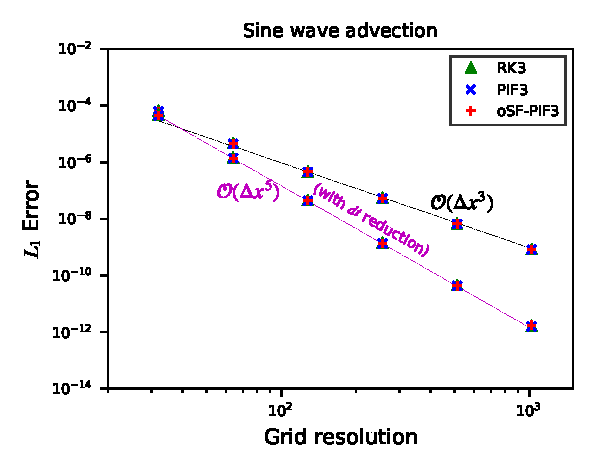
\includegraphics[width=0.85\textwidth]{fig/sine_over_dtReduction}
    \caption{Convergence test for the 1D sine wave advection problem.
        The errors are calculated
        in \( L_{1} \) sense against the initial density profile
        resolved on the computational grids refined
        from 32 to 1024 by a factor of 2.
        All numerical solutions follow the theoretical third-order convergence rate
        (the black-dotted line) when using the timesteps 
        computed from the Courant condition.
        Also plotted are the solutions of using reduced timesteps, which follows the
        fifth-order convergence rate represented in the pink-dotted line.
    }\label{fig:sine_wave}
\end{figure}

The simulation domain is defined on a one-dimensional box of \( [0, 1] \)
with the periodic boundary condition on both ends.
The density profile will propagate one period through the computational domain
and will return to its initial position at \( t = 1 \).
In return, any shape deformation of the density profile
from the initial density profile can be considered as a numerical error
associated with phase errors or numerical diffusions.
The accuracy of the numerical solutions is measured by computing \( L_{1} \) error
between the initial and the final density profiles.
The numerical experiment results from the sine wave advection test
on different number of grid points, \( N_{x} = 32, 64, 128, 256, 512, \) and \( 1024 \)
are depicted in~\cref{fig:sine_wave} for three different temporal methods, Rk3, PIF3, and oSF-PIF3.

There are two types of convergence rates demonstrated in~\cref{fig:sine_wave}.
In the first type, the numerical solutions of three different temporal methods
advanced with timesteps computed from the Courant condition with \( C_{\text{cfl}} = 0.7 \).
Interestingly, the numerical solutions from all three different temporal methods
show a third-order convergence rate, indicating that the leading error term from
third-order temporal methods dominates the spatial error from the fifth-order WENO-JS method.
These results are different from~\cref{fig:vortex_error_saturation},
calculating \( L_{1} \) error from the 2D nonlinear vortex advection case,
where the solution accuracy follows the spatial order at low-resolution regions
until the leading error of the solution is caught up by the temporal error
as computational grids get further refined to higher resolutions.
However, in this test case, the third-order temporal accuracy quickly takes control
throughout the entire range of the grid resolutions tested herein.
This solution behavior strongly supports the importance of
integrating spatially reconstructed solutions with a temporal scheme whose accuracy is
sufficiently high enough to be well comparable to that of the spatial solver.

In the second type of the convergence rate, on the other hand, the timesteps are restricted
in order to match up the lower third-order temporal accuracy with the higher fifth-order spatial accuracy.
Following the usual trick of timestep reduction in~\cite{mignone2010high},
the timestep \( \Delta t_{N} \) is manually adjusted on a grid size of \( N \)
to satisfy the equal rate of change between the spatial and temporal variations.
The restricted timestep is defined by,
\begin{equation}\label{eq:dt_reduction}
    {\Delta t_N} = {\Delta t_0} \Big( \frac{\Delta x_N}{\Delta x_0} \Big)^{\frac{5}{3}},
\end{equation}
where the sub-indices ``0'' and \( N \) refer to the time and grid scales
on a nominal coarse and fine resolution, respectively.
In the current configuration, \( \Delta x_{0} \) is the grid-scale of \( N_{x} = 32 \),
and \( \Delta t_{0} \) is the corresponding timestep subject to the Courant condition with \( C_{\text{cfl}} = 0.7 \).
With the timestep reduction, the overall leading error from the spatial and temporal methods
are matched with the fifth-order spatial accuracy of WENO5,
and the numerical solution of PIF3 and oSF-PIF3 follows the fifth-order convergence rate as expected.
In all test cases for linear advection problems, the oSF-PIF3 solutions behave
almost equally well with the solutions of the original PIF3 and RK3 both quantitatively and qualitatively.



\subsection{Nonlinear isentropic vortex advection}\label{subsec:vortex_weno}

The isentropic vortex advection problem~\cite{shu1998essentially} is one of the most popular benchmark tests
to measure the numerical method's accuracy and performance in the nonlinear case.
Although the problem is fully nonlinear, the exact solution always exists
in the form of its initial condition,
from which an isentropic vortex is advected through periodic boundaries in a 2D computational box.
The accuracy of a numerical method on a nonlinear problem
can be evaluated by comparing the final density profile with the initial condition.

The initial condition consists of a constant background mean flow with \( \rho = 1 \),
\( (u, v) = (1,1) \) and \( p =1 \) on the 2D computaional domain
with periodic boundary conditions.
The isentropic vortex is given by the velocity perturbations \( (\delta u, \delta v) \),
and the temperature perturbation \( \delta T \).
The perturbation terms are designed to set the constant entropy \( S \)
everywhere in the simulation domain, i.e., \( \delta S = 0 \).
The perturbations are given as,
\begin{equation}\label{eq:isentropic_vortex_initial}
    \left( \delta u, \delta v \right) = \frac{\epsilon}{2 \pi} e^{-\half \left( 1 - r^{2} \right)} (-y, x), \quad
    \delta T = - \frac{\left( \gamma - 1 \right) \epsilon^{2}}{8 \gamma \pi^{2}} e^{1 - r^{2}},
\end{equation}
where \( \epsilon = 5 \) is the vortex strength and \( r^{2} = x^{2} + y^{2} \).
The vortex is initially located at the domain center,
and it advects to the diagonal directions, then returns to its original position after one cycle.
The simulation domain size is doubled-up as \( [0, 20] \times [0, 20] \)
compared to the original setup in~\cite{shu1998essentially},
to prevent vortex-vortex couplings near the periodic boundaries
as reported in~\cite{spiegel2015survey}.

\begin{figure}
    \centering
    \begin{subfigure}{70mm}
        \centering
        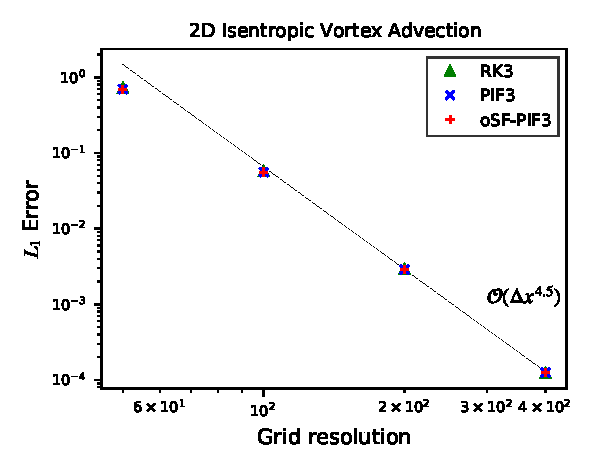
\includegraphics[width=0.95\textwidth]{fig/vortex_third}
    \end{subfigure}
    \begin{subfigure}{70mm}
        \centering
        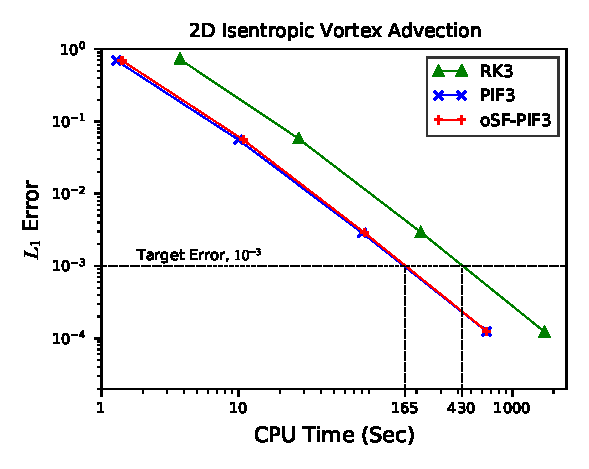
\includegraphics[width=0.95\textwidth]{fig/vortex_time_third}
    \end{subfigure}
    \caption{The \( L_{1} \) errors of the isentropic vortex advection test problem
        on different grid resolutions, \( N_{x} = N_{y} = 50, 100, 200, \) and \( 400 \).
        The three different third-order temporal schemes
        are used combined with WENO5 spatial method.
        The \( L_{1} \) errors
        with respect to the grid resolutions (\textbf{left});
        with respect to the computation time (\textbf{right}).
    }\label{fig:vortex_third}
\end{figure}

The results of the convergence test are depicted on the left panel in~\cref{fig:vortex_third}.
Three different temporal schemes, RK3, PIF3, and oSF-PIF3, show an excellent comparable match in
magnitudes and slopes of the \( L_{1} \) errors with varying grid resolution, \( N_{x} = N_{y} = 50, 100, 200, \) and \( 400 \).
One important finding in this figure is that there is no significant distinction
between PIF3 and oSF-PIF3 in accuracy and performance.
These results demonstrate that the original SF method
does not affect the solution accuracy and performance of the PIF method.

\begin{table}
    \centering
    \caption{The \( L_{1} \) errors, the rates of convergence,
        and the relative computation times for the vortex advection test.
        Here, the comparison between RK3 and oSF-PIF is only displayed,
        since the difference between oSF-PIF3 and PIF3 is indistinguishable.
        All the performance results (measured in seconds) are averaged
        over 10 simulation runs which are conducted on
        a Coffee Lake quad-core i7 Intel CPU with a
        clock speed of 2.7GHz, Turbo Boost up to 4.5GHz,
        utilizing four parallel threads.
    }\label{table:vortex_weno_third}
    \begin{adjustbox}{width=\textwidth}
        \begin{tabular}{@{}lcccclcccc@{}}
            \toprule
            \multirow{2}{*}{\( N_{x} = N_{y} \)} & \multicolumn{4}{c}{RK3} &  & \multicolumn{4}{c}{oSF-PIF3} \\
            \cmidrule(lr){2-5} \cmidrule(l){7-10}
            & \(L_{1}\) error & \(L_{1}\) order & CPU Time & Speedup &  &
            \(L_{1}\) error & \(L_{1}\) order & CPU Time & Speedup \\ \midrule
            50  & \num{7.22E-1} & \--- & \SI{3.73}{\second}    & 1.0 &  & \num{6.95E-1} & \--- & \SI{1.41}{\second} & 0.38 \\
            100 & \num{5.76E-2} & 3.65 & \SI{27.51}{\second}   & 1.0 &  & \num{5.58E-2} & 3.64 & \SI{10.82}{\second} & 0.39 \\
            200 & \num{2.94E-3} & 4.29 & \SI{214.44}{\second}  & 1.0 &  & \num{2.89E-3} & 4.27 & \SI{83.21}{\second} & 0.39 \\
            400 & \num{1.22E-4} & 4.59 & \SI{1727.71}{\second} & 1.0 &  & \num{1.26E-4} & 4.52 & \SI{652.18}{\second} & 0.38
        \end{tabular}
    \end{adjustbox}
\end{table}

The performance results of three different temporal schemes are presented
on the right panel of~\cref{fig:vortex_third} and summarized in~\cref{table:vortex_weno_third}.
Both the PIF3 and oSF-PIF3 methods perform more than two times faster than the multi-stage method, RK3.
It is worth noting that the original SF-PIF method, oSF-PIF, can be readily swappable
with an RK integrator in an existing code without too much effort,
leaving any existing spatial implementations intact.
Moreover, such a code transformation with oSF-PIF is more advantageous in simplicity
than the original PIF method because oSF-PIF replaces the analytic derivations of the Jacobian and Hessian terms
with the system-free approximations,
which have shown to be highly commensurate with
the analytical counterparts of the original PIF scheme.

Unlike the 1D linear sine advection test in~\cref{subsec:sine_wave},
the overall solution accuracy is not completely dominated by the third-order temporal discretizations,
which could reduce the overall convergence rate down to third-order as observed in the sine advection case.
Concurrently, the solution does not converge at full fifth-order either,
the rate due to the use of WENO5.
This can be explained as a nonlinear effect in which the lower third-order time integration schemes
slightly compromise the overall leading error term of the fifth-order spatial discretization.

\begin{figure}
    \centering
    \begin{subfigure}{70mm}
        \centering
        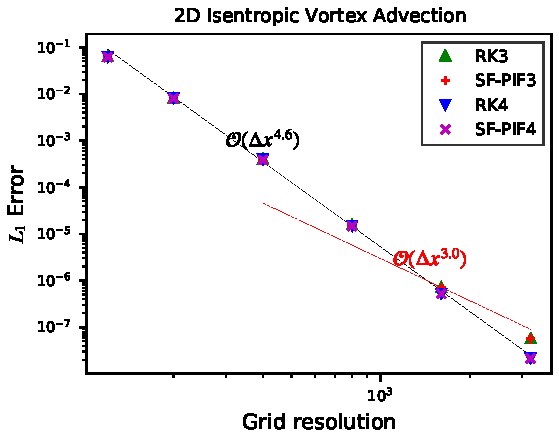
\includegraphics[width=0.95\textwidth]{fig/weno5_vortex_error_fourth}
    \end{subfigure}
    \begin{subfigure}{70mm}
        \centering
        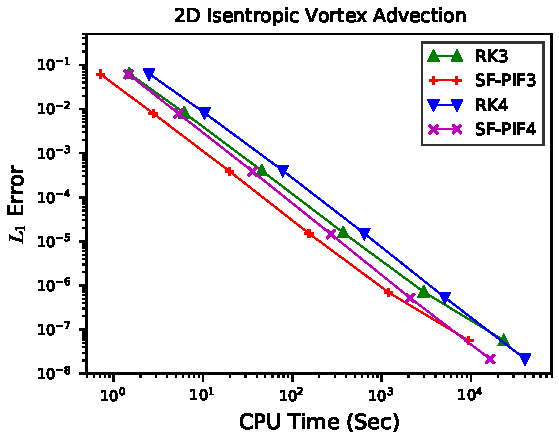
\includegraphics[width=0.95\textwidth]{fig/weno5_vortex_time_fourth}
    \end{subfigure}
    \caption{The \( L_{1} \) errors of the isentropic vortex advection test problem
        solved by third- and fourth-order temporal schemes combined with WENO5 spatial method.
        The \( L_{1} \) errors
        with respect to the grid resolutions (\textbf{left});
        with respect to the computation time (\textbf{right}).
    }\label{fig:vortex_fourth}
\end{figure}

However, the third-order temporal schemes gradually degrade the overall solution accuracy
on the fine grid resolutions. \cref{fig:vortex_fourth} illustrates the same convergence test results,
but in this case, containing more higher grid resolutions, \( N_{x} = N_{y} = 120, 200, 400, 800, 1600, \) and \( 3200 \).
Notice that the recursive SF-PIF method, SF-PIF3, and SF-PIF4 are used instead of the original SF-PIF method.
As expected, all temporal methods follow the convergence line of order \( \sim \mathcal{O}(\dx^{4.5}) \),
which is nearly the same as WENO's fifth-order spatial accuracy, equivalently in~\cref{fig:vortex_third}.
However, at the critical grid resolution, \( N_{x} = N_{y} = 1600 \),
the third-order temporal schemes of RK3 and SF-PIF3 start to compromise the overall solution accuracy.
This behavior can be explained that the spatial errors from the fifth-order WENO method
are dominant on the grid resolutions up to \( N_{x} = N_{y} = 1600 \),
after which the truncation errors associated with the third-order temporal methods
become dominant over the error of the fifth-order spatial solver, WENO5.
This result emphasizes the importance of high-order temporal methods in fine grid resolution:
a high-order spatial method does require a \textit{comparably} high-order temporal method
to maintain the overall quality of the solutions,
mainly when adding more grid resolutions to resolve finer scales more accurately.
Otherwise, lower-order accuracy from the temporal solver can potentially degrade
the solution accuracy, contradicting the intended motivation.

\begin{table}
    \centering
    \caption{The \( L_{1} \) errors, the rates of convergence,
        and the computation times for the vortex advection test
        solved using RK3 and SF-PIF3 methods (\textbf{top});
        using RK4 and SF-PIF4 methods (\textbf{bottom}).
        All simulation runs are equipped with WENO5 spatial method,
        performed on the four 20-cores
        Cascade Lake Intel Xeon processors, utilized 64 parallel threads.
        CPU times are measured in seconds, averaged over 10 individual runs.
    }\label{table:vortex_weno_fourth}
    \begin{adjustbox}{width=\textwidth}
        \begin{tabular}{@{}ccccclcccc@{}}
            \toprule
            \multirow{2}{*}{\( N_{x} = N_{y} \)} & \multicolumn{4}{c}{RK3} &  & \multicolumn{4}{c}{SF-PIF3} \\
            \cmidrule(lr){2-5} \cmidrule(l){7-10}
            & \(L_{1}\) error & \(L_{1}\) order & CPU Time & Speedup &  &
            \(L_{1}\) error & \(L_{1}\) order & CPU Time & Speedup \\ \midrule
            120  & \num{6.31E-2} & \--- & \SI{1.50}{\second}      & 1.0 &  & \num{6.16E-2} & \--- & \SI{0.71}{\second}    & 0.48 \\
            200  & \num{8.20E-3} & 4.00 & \SI{6.17}{\second}      & 1.0 &  & \num{7.96E-3} & 4.00 & \SI{2.77}{\second}    & 0.45 \\
            400  & \num{4.02E-4} & 4.35 & \SI{45.44}{\second}     & 1.0 &  & \num{3.86E-4} & 4.37 & \SI{19.89}{\second}   & 0.44 \\
            800  & \num{1.57E-5} & 4.68 & \SI{372.47}{\second}    & 1.0 &  & \num{1.51E-5} & 4.68 & \SI{153.92}{\second}  & 0.41 \\
            1600 & \num{7.18E-7} & 4.45 & \SI{2957.26}{\second}   & 1.0 &  & \num{6.95E-7} & 4.44 & \SI{1203.10}{\second} & 0.41 \\
            3200 & \num{5.72E-8} & 3.65 & \SI{23274.37}{\second}  & 1.0 &  & \num{5.60E-8} & 3.63 & \SI{9494.65}{\second} & 0.41 \\
        \end{tabular}
    \end{adjustbox}
    \begin{adjustbox}{width=\textwidth}
        \begin{tabular}{@{}ccccclcccc@{}}
            \toprule
            \multirow{2}{*}{\( N_{x} = N_{y} \)} & \multicolumn{4}{c}{RK4} &  & \multicolumn{4}{c}{SF-PIF4} \\
            \cmidrule(lr){2-5} \cmidrule(l){7-10}
            & \(L_{1}\) error & \(L_{1}\) order & CPU Time & Speedup &  &
            \(L_{1}\) error & \(L_{1}\) order & CPU Time & Speedup \\ \midrule
            120  & \num{6.30E-2} & \--- & \SI{2.50}{\second}       & 1.0 &  & \num{6.14E-2} & \--- & \SI{1.47}{\second}     & 0.59 \\
            200  & \num{8.15E-3} & 4.00 & \SI{10.42}{\second}      & 1.0 &  & \num{7.91E-3} & 4.01 & \SI{5.33}{\second}     & 0.51 \\
            400  & \num{4.01E-4} & 4.35 & \SI{78.47}{\second}      & 1.0 &  & \num{3.85E-4} & 4.36 & \SI{35.89}{\second}    & 0.46 \\
            800  & \num{1.51E-5} & 4.73 & \SI{641.50}{\second}     & 1.0 &  & \num{1.46E-5} & 4.72 & \SI{270.94}{\second}   & 0.42 \\
            1600 & \num{5.33E-7} & 4.82 & \SI{5115.47}{\second}    & 1.0 &  & \num{5.21E-7} & 4.81 & \SI{2091.20}{\second}  & 0.41 \\
            3200 & \num{2.17E-8} & 4.62 & \SI{40195.034}{\second}  & 1.0 &  & \num{2.15E-8} & 4.60 & \SI{16377.73}{\second} & 0.41 \\
        \end{tabular}
    \end{adjustbox}
\end{table}

The performance results of recursive SF-PIF methods can be found
on the right panel of~\cref{fig:vortex_fourth} and \cref{table:vortex_weno_fourth}.
As shown in the right panel of \cref{fig:vortex_fourth},
the SF-PIF3 method is the fastest method in reaching any given target \( L_{1} \) error threshold until \( N_{x} = 1600 \).
However, on any grid resolutions finer than the critical resolution, \( N_{x} = 1600 \),
SF-PIF3's \( L_{1} \) error drops to the third-order convergence rate,
which ultimately crosses the straight convergence line of SF-PIF4.
SF-PIF3's error will remain larger than the errors from the fourth-order temporal methods
as long as the convergence rate follows the pattern at the high-resolution trail.

On the other hand, it is distinctively superior to see that SF-PIF4's solution
reaches any fixed target error in a \textit{faster} CPU time than the third-order RK3's solution
while keeping the numerical errors as low as RK4 results at all grid resolution tested herein.
Remark that \cref{table:vortex_weno_fourth} shows quantitatively that
the SF-PIF4 method performs \textit{faster} than the RK3 method,
producing more accurate solutions at any grid resolution.







\subsection{Sod shock tube problem}\label{subsec:sod}

The Sod's shock tube problem~\cite{sod1978survey} is the one of the most famous 1D hydrodynamics
test problems for testing a numerical scheme's capability to handle discontinuities and shocks.
The initial condition is given as,
\begin{equation}\label{eq:sod_init}
    \left( \rho, u, p \right) = \begin{cases}
        \left( 1, 0, 1 \right) & \text{for } x \le 0.5, \\
        \left( 0.125, 0, 0.1 \right) & \text{for } x > 0.5,
    \end{cases}
\end{equation}
in a simulation box of \( [0, 1] \), with outflow boundary conditions
on both ends at \( x = 0 \) and \( x = 1 \).
This benchmark problem is an excellent practice to
test if the PIF and oSF-PIF methods can be capture the shock discontinuities
appropriately.

\begin{figure}
    \centering
    \begin{subfigure}{0.49\textwidth}
        \centering
        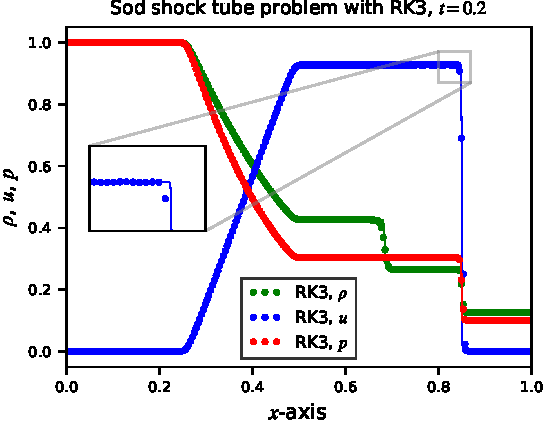
\includegraphics[width=\textwidth]{fig/sod_rk3}
        \caption{}\label{subfig:sod_rk3}
    \end{subfigure}
    \begin{subfigure}{0.49\textwidth}
        \centering
        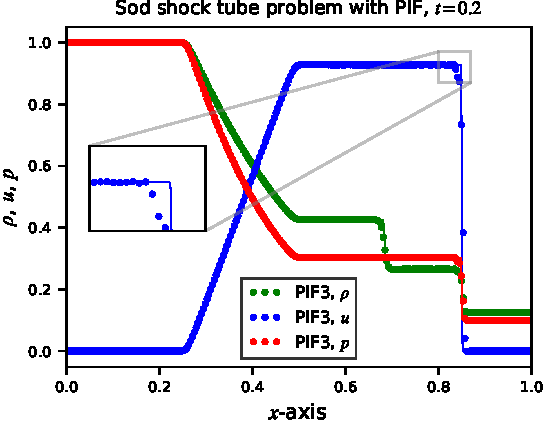
\includegraphics[width=\textwidth]{fig/sod_pif3}
        \caption{}\label{subfig:sod_pif3}
    \end{subfigure}
    \begin{subfigure}{0.49\textwidth}
        \centering
        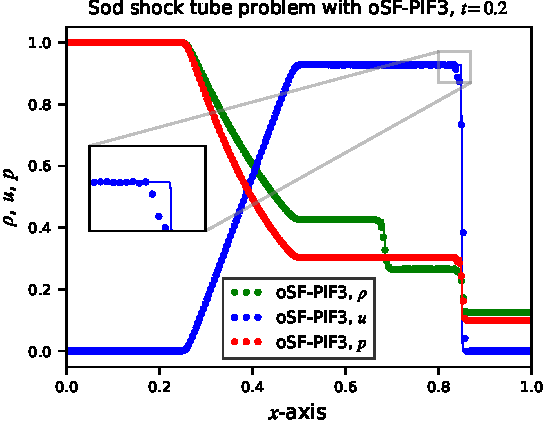
\includegraphics[width=\textwidth]{fig/sod_osf3}
        \caption{}\label{subfig:sod_osf3}
    \end{subfigure}
    \begin{subfigure}{0.49\textwidth}
        \centering
        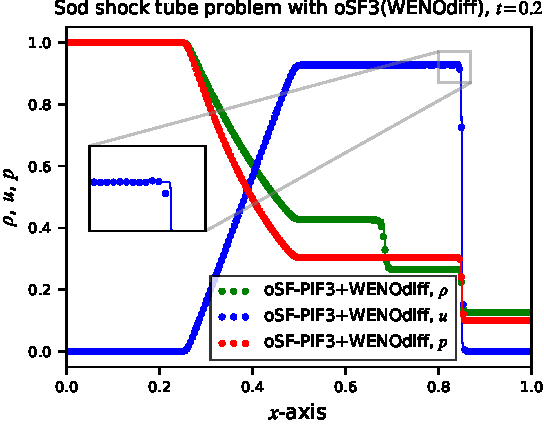
\includegraphics[width=\textwidth]{fig/sod_osf3_wenodiff}
        \caption{}\label{subfig:sod_osf3_wenodiff}
    \end{subfigure}
    \caption{Sod's shock tube problem at \( t = 0.2 \).
        The reference solutions are over-plotted
        as solid lines in each panel, which are resolved on a grid resolution of \( N_{x} = 1024 \)
        with RK3. The symbols in each panel represent the solution resolved on
        \( N_{x} = 256 \) grid cells with
        (\protect\subref{subfig:sod_rk3}) RK3,
        (\protect\subref{subfig:sod_pif3}) PIF3, and (\protect\subref{subfig:sod_osf3}) oSF-PIF3\@.
        (\protect\subref{subfig:sod_osf3_wenodiff}), the solution is resolved
        with oSF-PIF3 method combining with a new WENO-\textit{like} numerical differentiate operator,
        described as in~\crefrange{eq:pif_wenodiff_subs}{eq:pif_wenodiff_linear_weights}.
    }\label{fig:sod_third}
\end{figure}

The numerical solutions with the grid size of \( N_{x} = 256 \) at \( t = 0.2 \) are plotted
as symbols in each panel of~\cref{fig:sod_third}.
The solid lines on each panel represent the reference solution resolved on a more finer grid size,
\( N_{x} = 1024 \), by using WENO5+RK3.
The results resolved with recursive SF-PIF3 methods are omitted in this figure,
since the differences between SF-PIF3 and oSF-PIF3 are indistinguishable.

As illustrated in~\cref{subfig:sod_pif3} and~\cref{subfig:sod_osf3},
oSF-PIF3 method produce almost identical results of PIF3,
agreeing with the reference solutions and RK3's solutions in~\cref{subfig:sod_rk3}.
However, both in PIF3 and oSF-PIF3 methods,
there is a slight oscillation in the x-velocity immediately behind the shock front.
This small oscillation is originated from the use of
the conventional central differencing formulae in~\cref{eq:pif_central_dfdx}
for both oSF-PIF3 and PIF3.

The WENO-\textit{like} differencing strategy in~\crefrange{eq:pif_wenodiff_subs}{eq:pif_wenodiff_linear_weights}
can resolve this oscillation. As displayed in~\cref{subfig:sod_osf3_wenodiff},
the interchanging central differencing to WENO-differencing helps
to improve the performance of oSF-PIF3 at the shock,
suppressing the post-shock oscillations observed in~\cref{subfig:sod_pif3} and~\cref{subfig:sod_osf3}.
With this small fix, the oSF-PIF3 results are almost identical to the RK3 results in~\cref{subfig:sod_rk3}.
Computationally, the WENO-\textit{like} differencing adds extra floating-point operations,
which consequently slows down oSF-PIF's and SF-PIF's overall performance.
For this reason, the WENO-\textit{like} discretization was employed only
on the Sod's shock-tube test as a guide,
while it was opt-out on the rest of the test problems in this dissertation
where any unphysical has not been observed shock/discontinuity oscillations.


\subsection{Implosion test}\label{subsec:implosion}

The next problem to consider is the implosion test problem
introduced by Hui et al.~\cite{hui1999unified}.
An unsteady flow configuration is given as an initial condition which launches
a converging shock wave towards the domain center.
Following a more straightforward version by Liska and Wendroff~\cite{liska2003comparison},
the only right upper quadrant
of the original setup in~\cite{hui1999unified} is taken
as the simulation domain.
In this setup, the simulation is initialized on a region of a 2D square box,
\( \left[ 0, 0.3 \right] \times \left[ 0, 0.3 \right] \),
enclosed with reflecting walls,
in which case a converging shock wave is launched toward the lower-left corner
at $(x,y)=(0,0)$.
The initial shock wave bounces at the reflecting walls and produces a double Mach
reflection along two edges of $x=0$ and $y=0$.
Consequently, two jets are formed along the edges, moving toward the origin $(x,y)=(0,0)$ and collide
with each other. This two-jet collision then ejects a newly-formed jet into the diagonal direction
$x=y$. Reflecting shocks continuously interact with the diagonal jet, turning it into
a long and narrow shape over time. The observed structures of filaments and fingers
along with the diagonal jet and at its base are progressively intensified by the
Ritchmyer-Meshkov instability, a level of which depends sensitively on
numerical dissipation.

The shape of the jet is the key view point of
the implosion test since it is a good indicator of
a numerical method's symmetric property and numerical dissipation.
If the numerical scheme fails to maintain a high level of symmetry,
the jet will eventually be derailed off-diagonally and deformed over time.
Besides, an excess amount of numerical dissipation will
turn the jet into a less narrow and less elongated shape along the diagonal.

\begin{figure}
    \centering
    \begin{subfigure}{70mm}
        \centering
        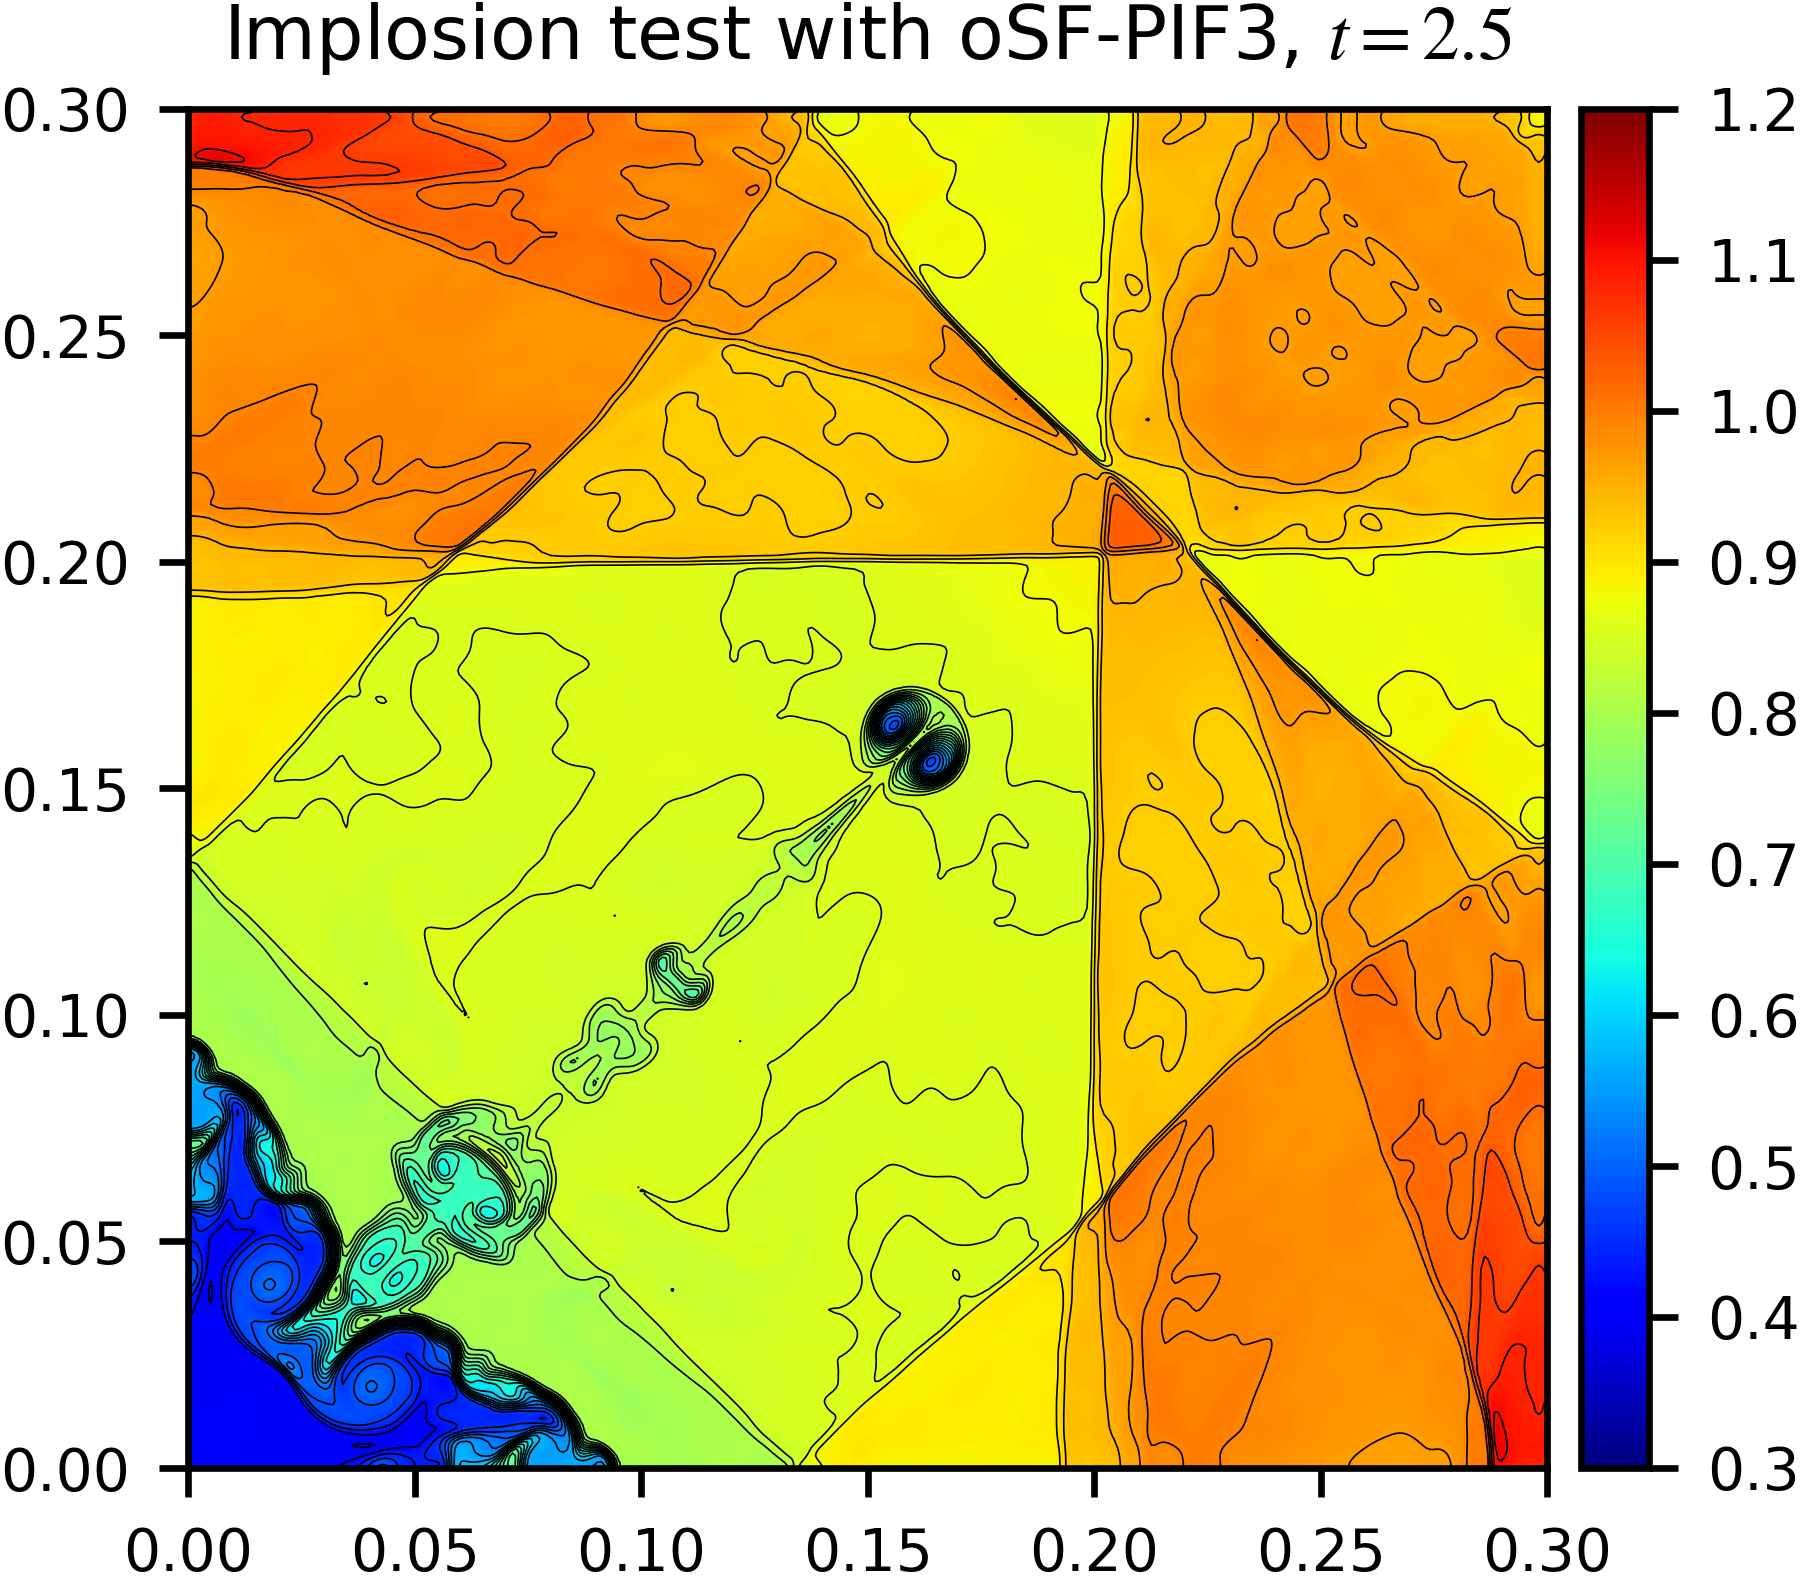
\includegraphics[width=0.95\textwidth]{fig/implosion_osf3.png}
    \end{subfigure}
    \begin{subfigure}{70mm}
        \centering
        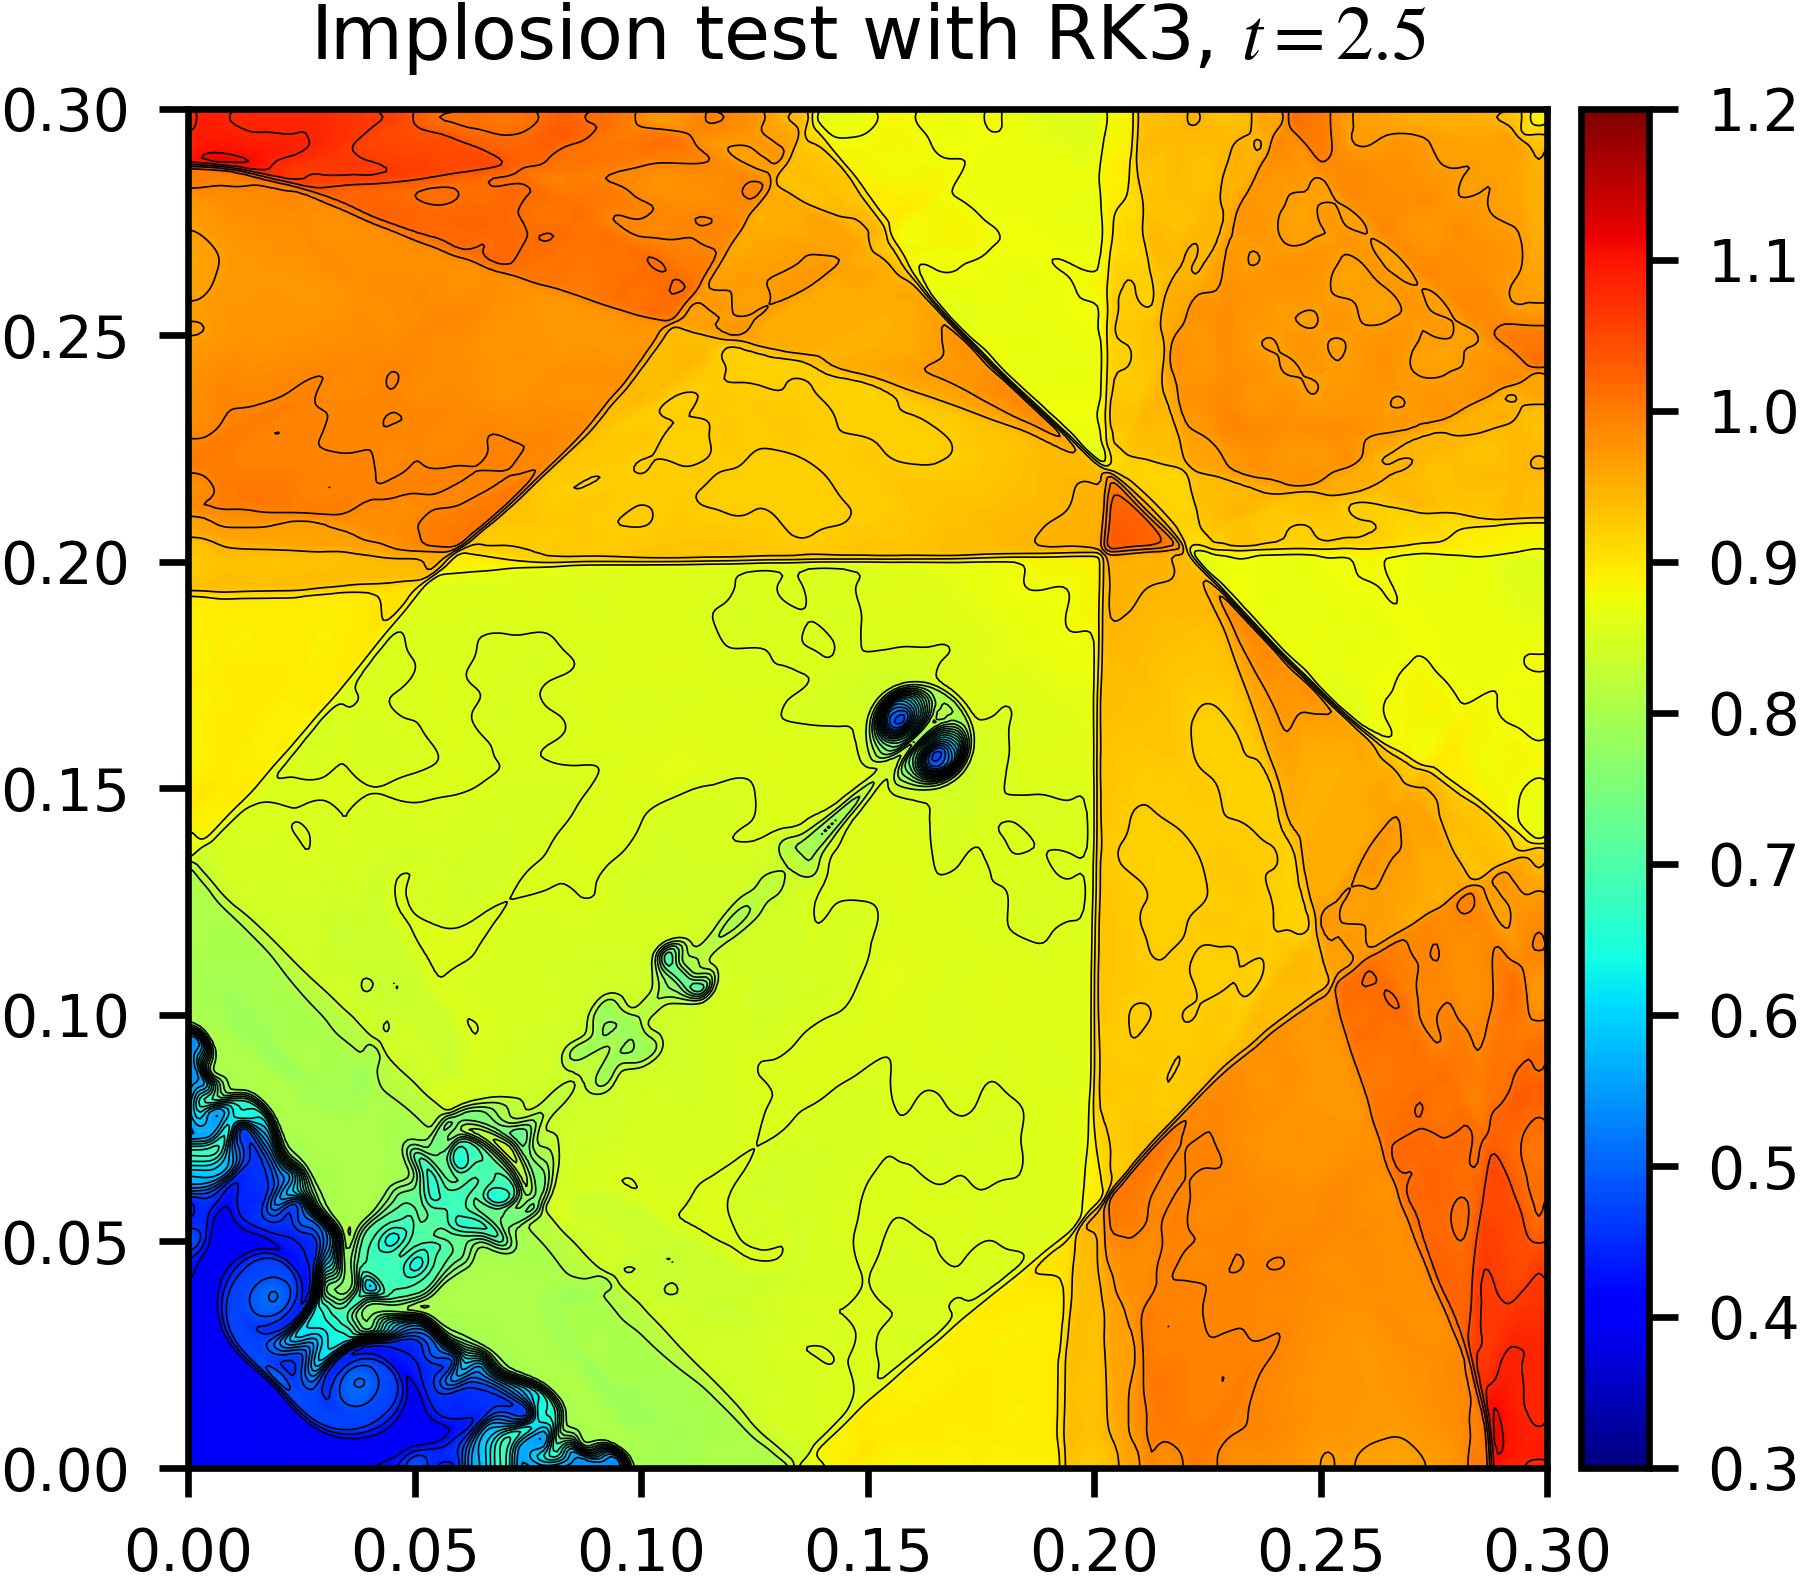
\includegraphics[width=0.95\textwidth]{fig/implosion_rk3.png}
    \end{subfigure}
    \caption{The density profile of the implosion test
        with oSF-PIF3 (left) and with RK3 (right).
        The color map ranges from \( 0.3 \) to \( 1.2 \), and
        40 evenly-spaced contour lines are over-plotted with
        the same range.
    }\label{fig:implosion}
\end{figure}

The density maps of the implosion test performed on
\( 400 \times 400 \) grid resolution at \( t = 2.5 \) are displayed in~\cref{fig:implosion}.
The result with oSF-PIF3 is on the left panel in \cref{fig:implosion} and RK3 on the right.
These results can also be directly compared with
Fig.~4.7 in~\cite{liska2003comparison} and Fig.~17 in~\cite{stone2008athena}.
The results of oSF-PIF3 (as well as RK3) present
the well-maintained symmetric jet along the diagonal direction
at a sufficient level.
At the same time, the shape of the diagonal jet using oSF-PIF3 matches
well with the shape using RK3,
and hence is sufficient to demonstrate that the numerical dissipation in oSF-PIF3
is well-managed compared with RK3.


\subsection{Shallow water equations}\label{subsec:shallow}

One of the essential features of the SF-PIF methods is that the SF-PIF methods
can be applicable to any other system without changing the high-order parts of the simulation codes.
As an example of the system independence feature,
the simulation result by changing the system of equations to the 2D shallow water equations (SWE)
without a source term is presented in this section.
In SWE, the conservative variables and the flux functions are defined by,
\begin{equation}\label{eq:swe_gov}
    \bU = \begin{bmatrix}
        h \\
        h u \\
        h v
    \end{bmatrix},\quad
    \bF (\bU) = \begin{bmatrix}
        h u \\
        h u^{2} + \frac{1}{2} g h^{2} \\
        h u v
    \end{bmatrix}, \quad
    \bG (\bU) = \begin{bmatrix}
        h v \\
        h u v \\
        h v^{2} + \frac{1}{2} g h^{2}
    \end{bmatrix}.
\end{equation}
Here, \( h \) is the vertical depth of the fluid,
\( \mathbf{v} = \left( u, v \right)  \) is a vector of 
vertically-averaged velocity components in $x$- and $y$-directions.
Denoted as \( g \) is a gravitational acceleration in the negative vertical 
$z$-direction, which is averaged out in the derivation of the shallow water equations.

The sole purpose of presenting the new system of equations above
is to demonstrate the flexibility of SF-PIF schemes,
in that the system-free approach allows an easy code implementation
without the need for other analytical derivations of new
Jacobian-\textit{like} terms of the new governing system.
By virtue of the system-independent property of the SF-PIF methods,
the process of changing from the 2D Euler code to the 2D SWE code is
no more than switching the governing equations
without touching anything on the high-order numerical parts.
This process is much simpler than other Lax-Wendroff type schemes (PIF, for example),
where each governing system should re-calculate the Jacobian-\textit{like} terms.

The well-known circular dam-breaking problem~\cite{alcrudo1993high,toro2001shock,delis2005numerical}
is conducted to validate the numerical capability of the SF-PIF method in SWE\@.
Initially, a volume of still water is confined
in the virtual (i.e., invisible) cylindrical 
wall with a radius of 11 meters (m),
located at the center of simulation domain,
\( \left[ \SI{50}{\meter} \times \SI{50}{\meter} \right] \)
resolved on a $100 \times 100$ grid resolution.
The depth of the water inside of the wall is
\( \SI{10}{\meter} \) and \( \SI{1}{\meter} \) outside.
This configuration would be considered as an
SWE version of 2D Riemann problem.
Explicitly, the initial condition is given as,
\begin{equation}\label{eq:swe-init}
    \left(h, u, v \right) = \begin{cases}
        \left(\SI{10}{\meter}, 0, 0 \right) & \text{for } r \le \SI{11}{\meter}, \\
        \left(\SI{1}{\meter}, 0, 0 \right) & \text{for } r > \SI{11}{\meter}, \\
    \end{cases}
\end{equation}
where \( r \) is the distance from the center of domain,
\( r = \sqrt{\left( x - \SI{25}{\meter} \right)^{2} + \left( y - \SI{25}{\meter} \right)^{2} } \).
The outflow boundary condition is applied for both directions,
and the gravitational acceleration is \( g = \SI{9.81}{\meter\per\square\second}\).
Again, the Courant number is set to \( C_{\text{cfl}} = 0.4 \).

\begin{figure}
    \centering
    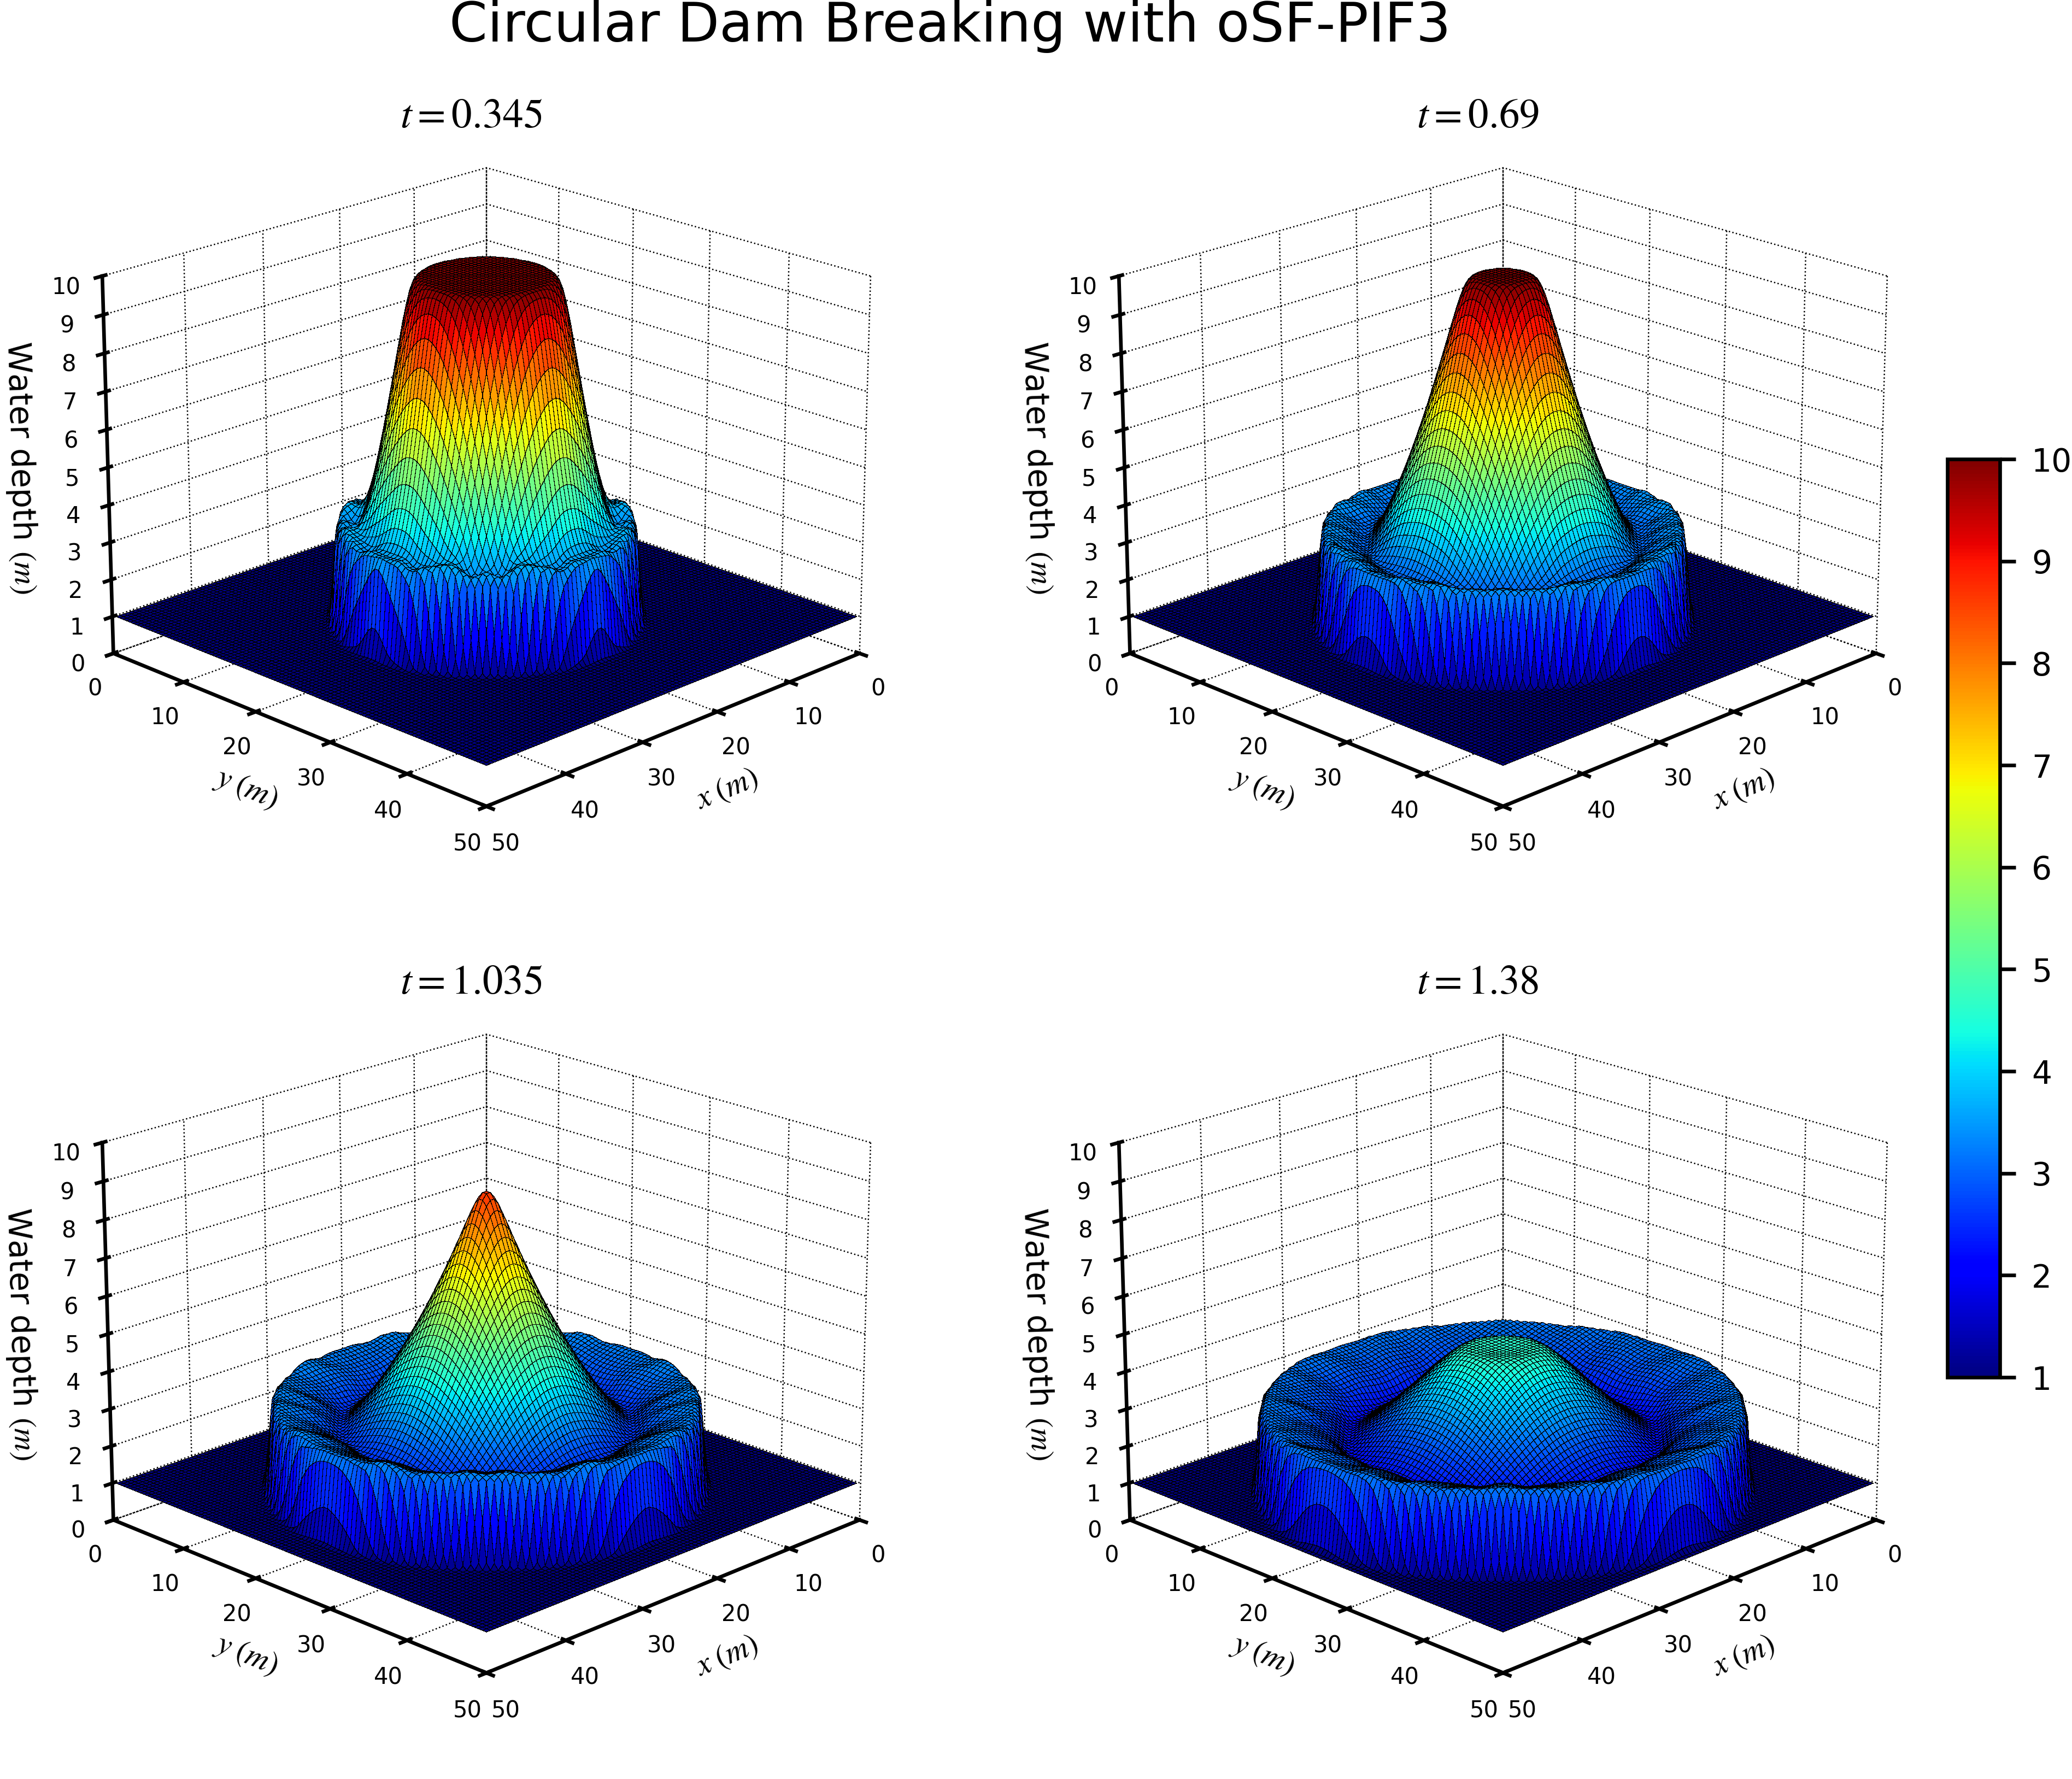
\includegraphics[width=\textwidth]{fig/swe_circ_osf3_all.png}
    \caption{Snapshots of the circular dam breaking simulation
        at four different times, \( t = 0.345, 0.69, 1.035, \) and $1.38$ seconds.
        A volume of water in rest is initially confined
        in a cylindrical dam of a radius $r=11$ m and a height $h=10$ m.
        The simulation starts with an instantaneous removal of the cylindrical wall
        located at the center of the domain
        \( \left[ \SI{50}{\meter} \times \SI{50}{\meter} \right] \)
        resolved on a grid resolution of $100 \times 100$.
        The gravitational force is exerted on the steady water,
        which triggers the onset of the gravitational collapse of the entire volume of water,
        making the circular splash in the outer rim as well as the ripple effects
        in the central region that move radially outward in time.
    }\label{fig:swe_circ}
\end{figure}

The results of the simulation with the oSF-PIF3 method are presented in~\cref{fig:swe_circ}.
The figure represents well-comparable numerical solutions
with the results using the same configuration
reported in~\cite{alcrudo1993high,toro2001shock,delis2005numerical}.
As shown in \cref{fig:swe_circ}, the overall spherical symmetry and the sharp profile
at the wavefront are well-maintained in each snapshot
at four different times, \( t = 0.345, 0.69, 1.035, \) and \( 1.38 \).



\section{SF-PIF method with WENO-JS}\label{sec:result_wenojs}

The previous section demonstrates that the original SF-PIF and recursive SF-PIF methods,
combined with the traditional WENO method,
generate the highly accurate and stable solution in faster computational time
compared to the SSP-RK methods.
This section provides numerical test results from additional benchmark problems,
both in 2D and 3D, with the presence of strong shock.
All simulations are performed with third-order and fourth-order \textit{recursive} SF-PIF methods
coupled with the traditional fifth-order WENO method described in~\cref{subsec:weno}.
2D simulations are carried out on high grid resolutions
to emphasize the numerical effects of the temporal solver, as discussed in~\cref{subsec:vortex_weno}.

\subsection{The Shu-Osher problem (rotated \(\ang{45}\))}\label{subsec:shu45_weno}

The Shu-Osher problem~\cite{shu1989efficient} is a well-known benchmark problem
that describes the interactions between a Mach 3 shock and a smooth density profile.
Initially, a Mach 3 shock wave travels to the right through a sinusoidally perturbed
density profile. As the shock wave propagates along the perturbed region,
the profile gets compressed, resulting in a frequency-doubled region behind the shock. 
As the shock wave moves further to the right,
the doubled-frequency region returns to its original frequency, at which point
it becomes a sequence of sharp profile instead of smooth sine wave
due to the shock-steepening.

In this section, the Shu-Osher problem is performed in 2D by inclining the shock wave direction
by an angle of \(\theta = \ang{45} \),
adopting the idea of Kawai~\cite{kawai2013divergence},
where the initial conditions are repeated multiple times along the direction of the
wave propagation so that the problem may be executed with periodic boundary conditions.
Explicitly, the initial condition is given as,
\begin{equation}\label{eq:shu45_gov}
    \begin{split}
        &\bU(x_{\parallel}, t=0) = \begin{cases}
            \bU_{L} & \text{for } x_{\parallel} \le 1, \quad 11 < x_{\parallel} \le 21, \quad 31 < x_{\parallel} \le 40, \\
            \bU_{R} & \text{for } 1 < x_{\parallel} \le 11, \quad 21 < x_{\parallel} \le 31,
        \end{cases}\\
        &\text{where } \bU_{L} = \begin{bmatrix}
            \rho = 3.857143 \\
            u = 2.629369\cos(\pi/4) \\
            v = 2.629369\sin(\pi/4) \\
            p = 10.33333
        \end{bmatrix},\quad
        \bU_{R} = \begin{bmatrix}
            \rho = 1 + 0.2\sin(5 x_{\parallel}) \\
            u = 0 \\
            v = 0 \\
            p = 1
        \end{bmatrix}.
    \end{split}
\end{equation}

\begin{figure}
    \centering
    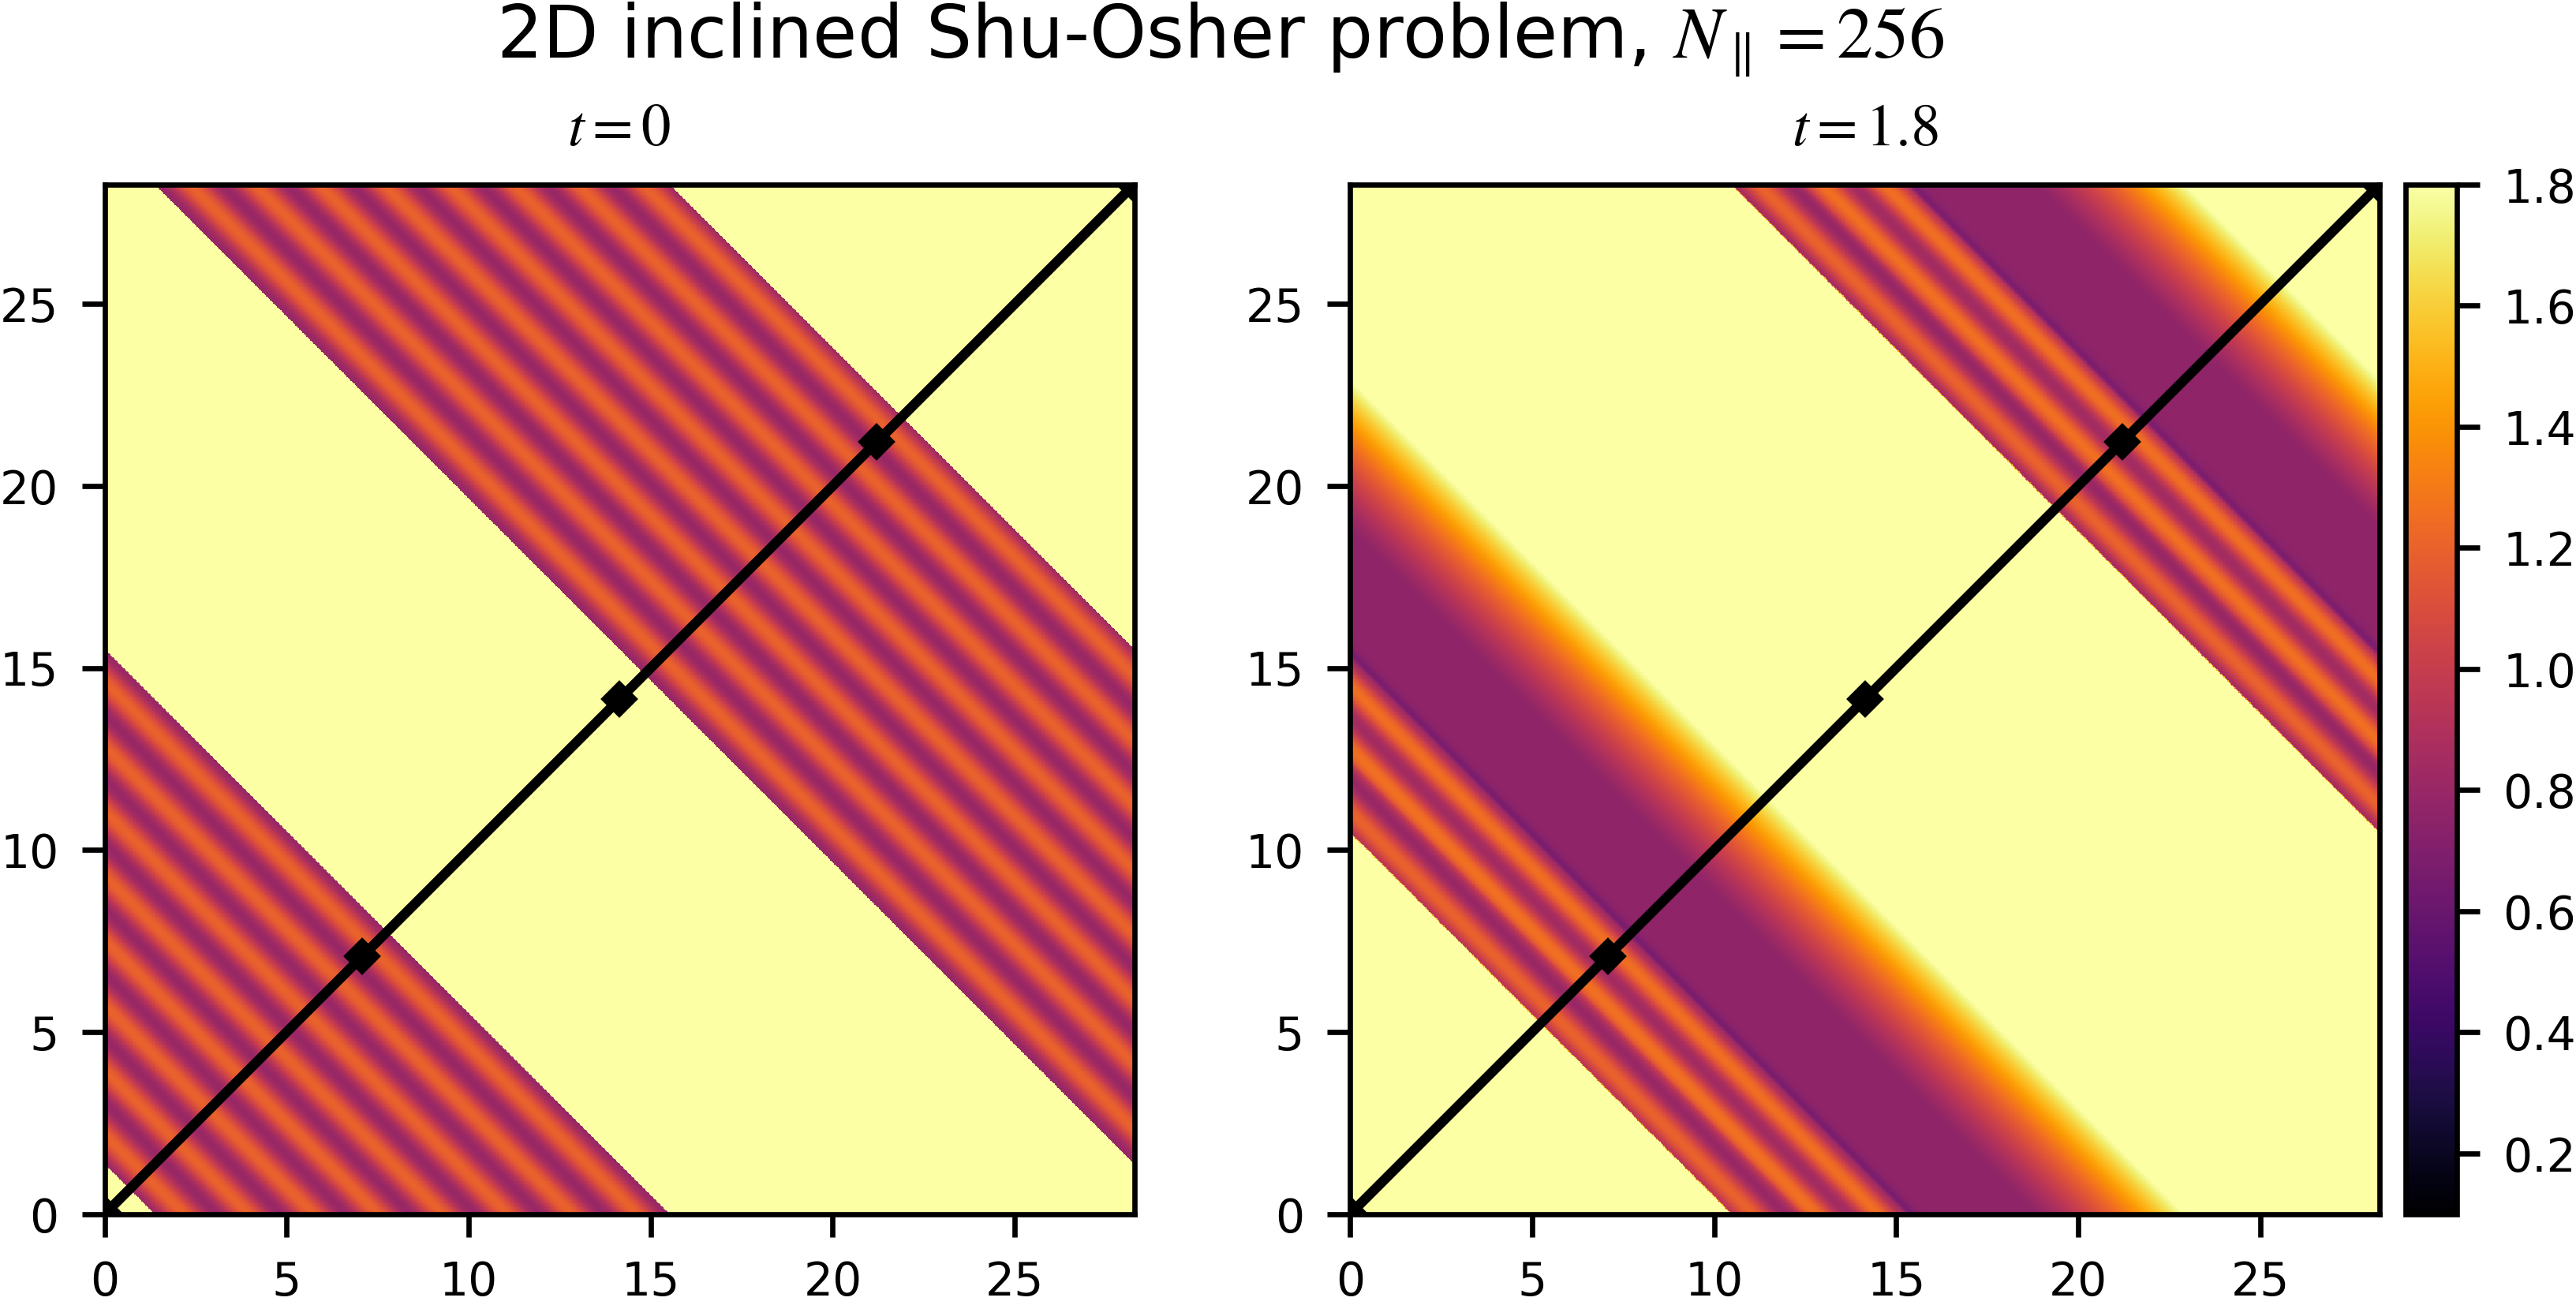
\includegraphics[width=0.95\textwidth]{fig/shu45_2d_snapshot.png}
    \caption{2D density maps of inclined 2D Shu-Osher test problem
        at \( t=0 \) and \( t=1.8 \). The test was performed on a 2D simulation box
        of \(1024 \times 1024 \) resolution with the SF-PIF4 method.
        The solid black line represents the shock propagating direction, \( x_{\parallel} \),
        and squares divide the line in each quartile.
    }\label{fig:shu45_cmap}
\end{figure}

\( x_{\parallel} = x \cos{\theta} + y \sin{\theta} \) is the direction
parallel to the wave propagation and the simulation domain is a periodic box of
\( [0, 20/\cos{\theta}] \times [0, 20/\sin{\theta}] \).
With this configuration, the 1D test problem, Shu-Osher test,
can be performed on the diagonal direction of 2D periodic box.
The same 1D solution is expected by following the diagonal direction, \( x_{\parallel} \),
and taking only the bottom-left quarter of the diagonal axis.
Therefore, the number of data points of this result profiles
would be a quarter of the 2D grid resolution,
i.e., \( N_{\parallel} = N_{x}/4 = N_{y}/4 \).
The 2D density map of the initial and final conditions are plotted in~\cref{fig:shu45_cmap}.

\begin{figure}
    \centering
    \begin{subfigure}{70mm}
        \centering
        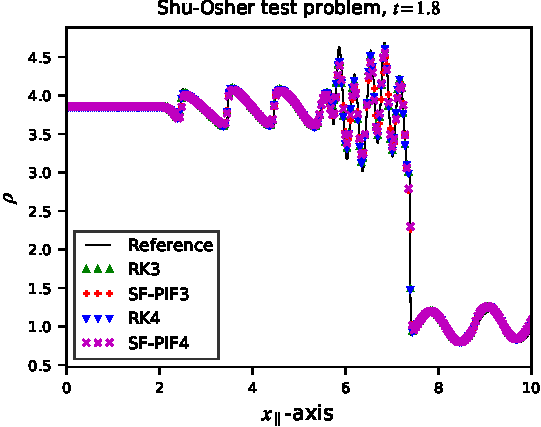
\includegraphics[width=0.95\textwidth]{fig/shu45_weno5_256}
    \end{subfigure}
    \begin{subfigure}{70mm}
        \centering
        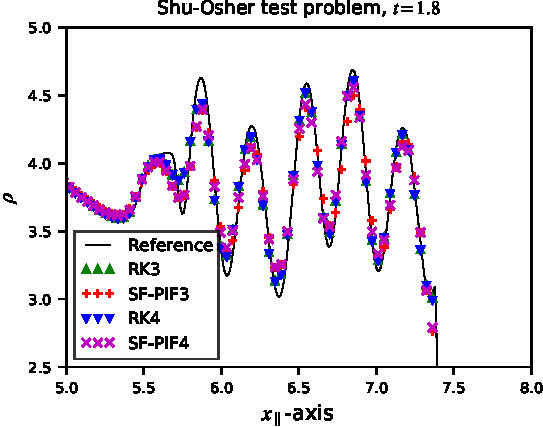
\includegraphics[width=0.95\textwidth]{fig/shu45_weno5_256_zoomed}
    \end{subfigure}
    \caption{One dimensional density profiles along the \( x_{\parallel} \) direction 
        of the inclined Shu-Osher problem at \( t = 1.8 \).
        The solid line represents the reference solution,
        solved by RK4 with 1024 data points
        in the diagonal axis, i.e., \( N_{\parallel} = 1024 \).
        All other solutions, represented by the symbols, are resolved on an
        \( N_{\parallel} = 256 \) grid resolution in the diagonal axis.
        The detailed view of the high-frequency region is shown
        on the right panel.
    }\label{fig:shu45}
\end{figure}

The density profiles of the bottom-left quarter of the diagonal axis \( x_{\parallel} \)
are given in~\cref{fig:shu45}. All tests are performed on a box of resolution \( N_{x} = N_{y} = 1024 \),
so the effective resolution of each profile is \( N_{\parallel} = 256 \),
except for the reference solution, which performed on a finer grid, \( N_{\parallel} = 1024 \).
The four different temporal methods, RK3, RK4, SF-PIF3, and SF-PIF4 produce
reasonably acceptable solution profiles capturing the high-frequency amplitudes
fairly well in the frequency-doubled region.
Generally, RK methods capture the amplitudes marginally better,
but in the left-most part of the double-frequency region, \( x \approx 5.8 \),
SF-PIF methods capture the highest peak of the amplitude better than
the RK methods near the transition between the frequency 
doubling and the shock steepened perturbations.




\subsection{2D Riemann problem: Configuration 3}\label{subsec:2drp_c3_weno}

The two-dimensional Riemann problem is a widespread benchmark problem to test
the methods' ability to capture the complex fluid structures in 2D.
This specific setup and other types of configurations have been
extensively studied in~\cite{zhang1990conjecture, schulz1993classification, schulz1993numerical}
and have been adopted as prevalent benchmark test problems.
This dissertation follows the initial condition of Configuration 3
described in~\cite{don2016hybrid,lee2017piecewise,lee2021single,lee2021recursive}.

The simulation domain is set on \( 1600 \times 1600 \) grid resolution,
which is generally considered as a very high resolution in 2D simulation.
This grid resolution choice is made based on the observation in~\cref{subsec:vortex_weno}
to ensure that the temporal errors are comparable to or dominant over the spatial errors;
thereby, the temporal error dominant results are anticipated that allows
to see the different behaviors of four different temporal solvers.

\begin{figure}
    \centering
    \begin{subfigure}{140mm}
        \centering
        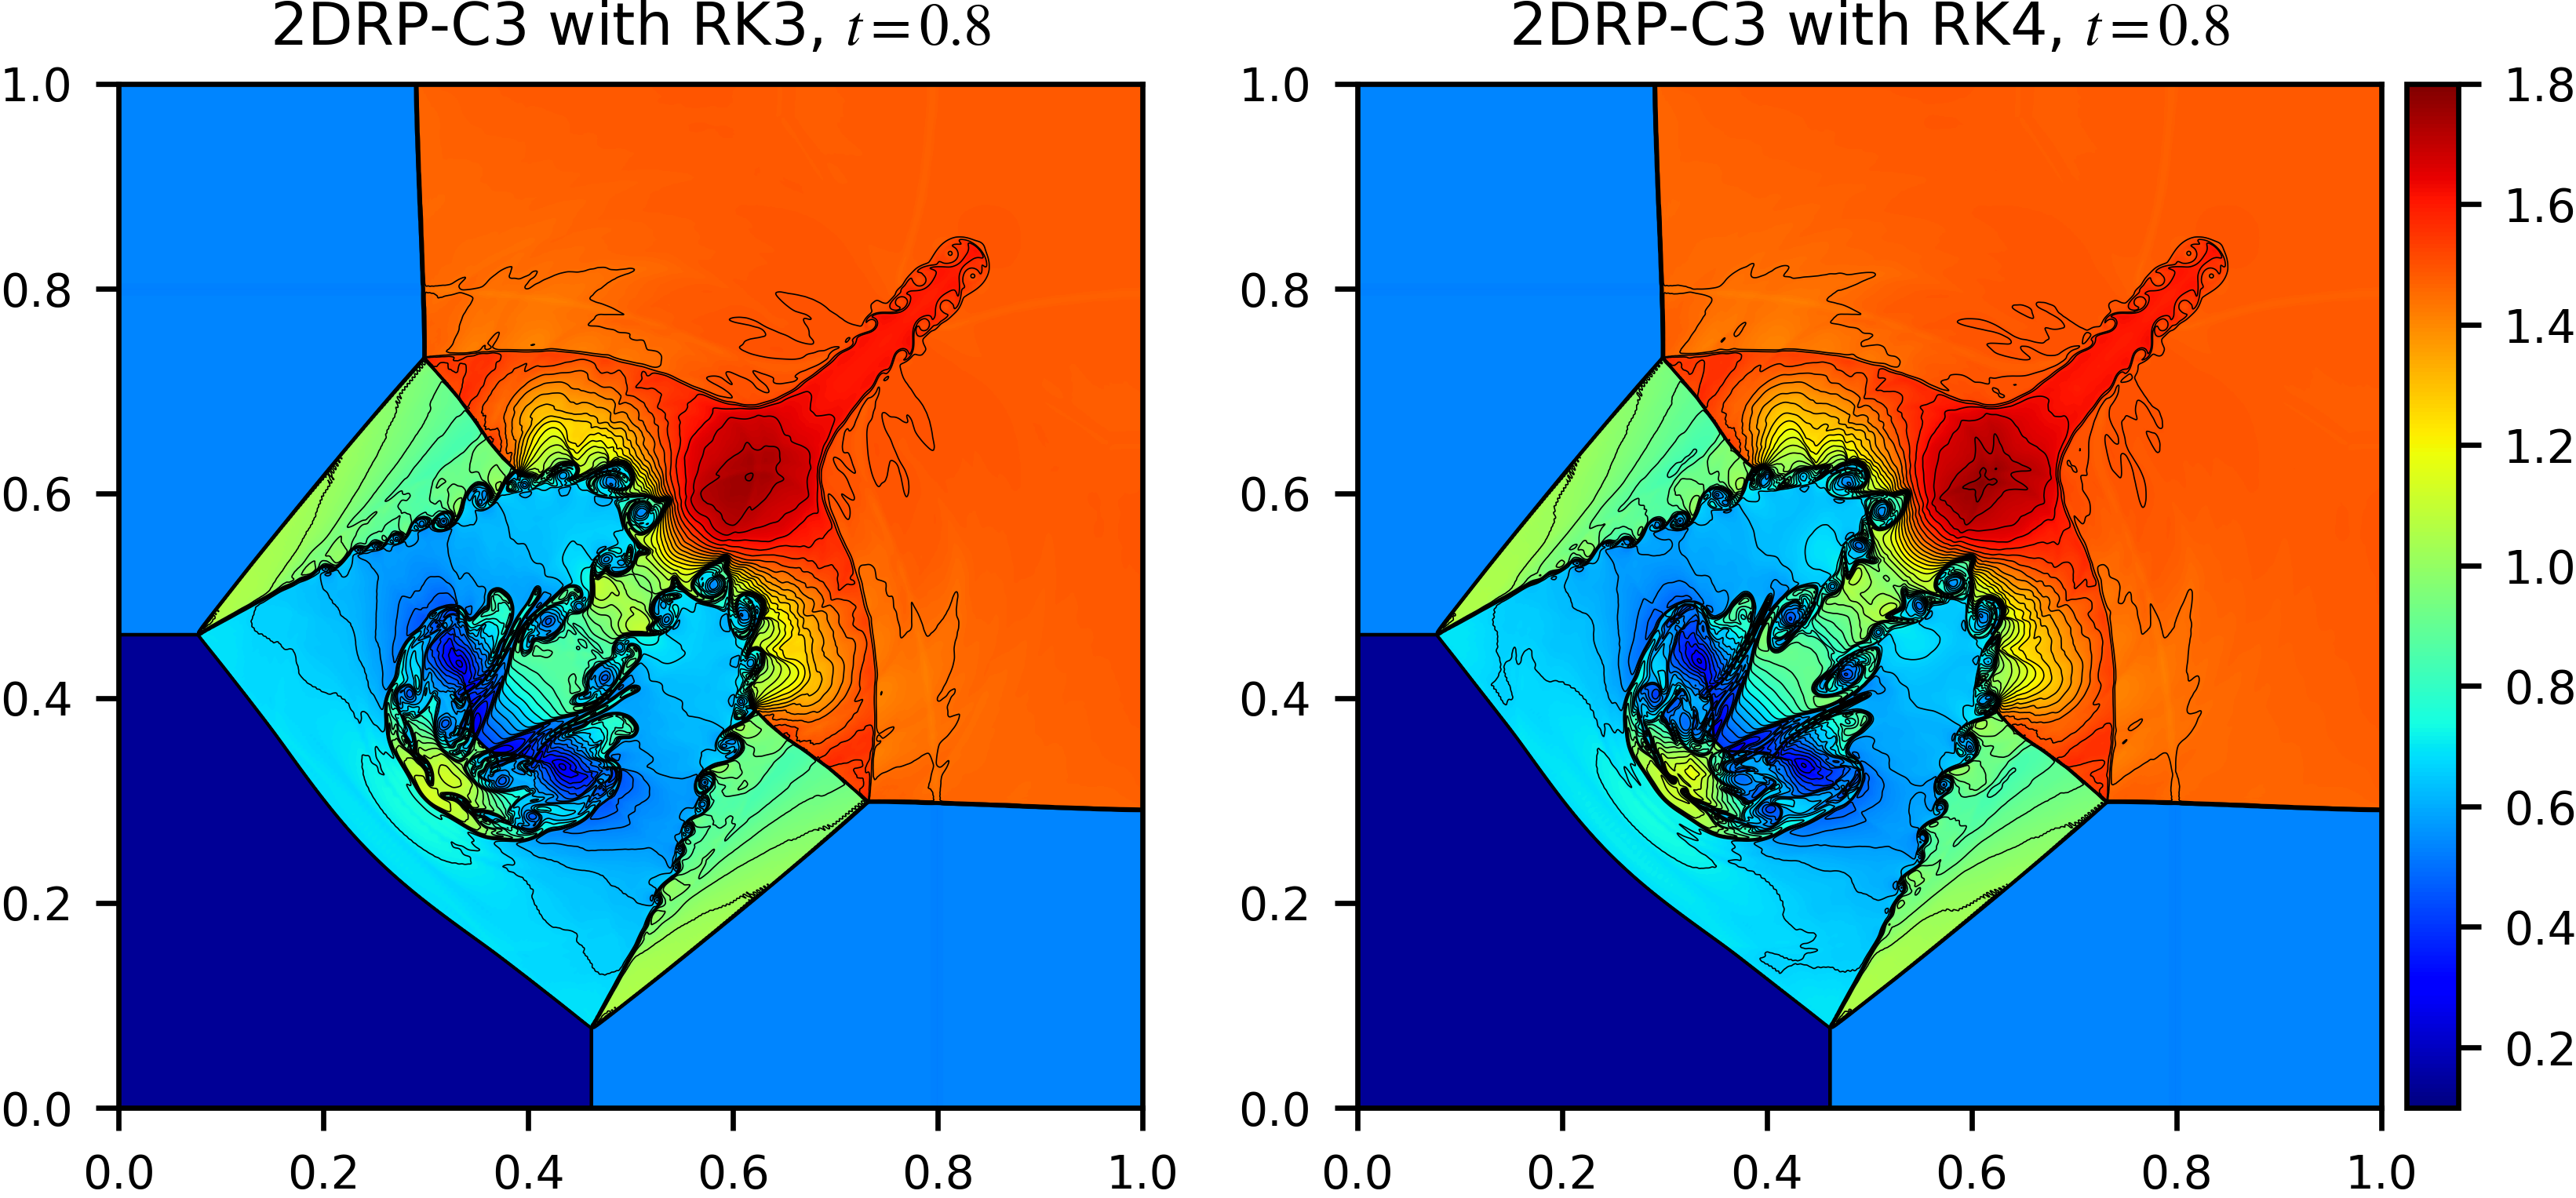
\includegraphics[width=0.9\textwidth]{fig/2drp_c3_weno5_rk_1600.png}
    \end{subfigure}
    \begin{subfigure}{140mm}
        \centering
        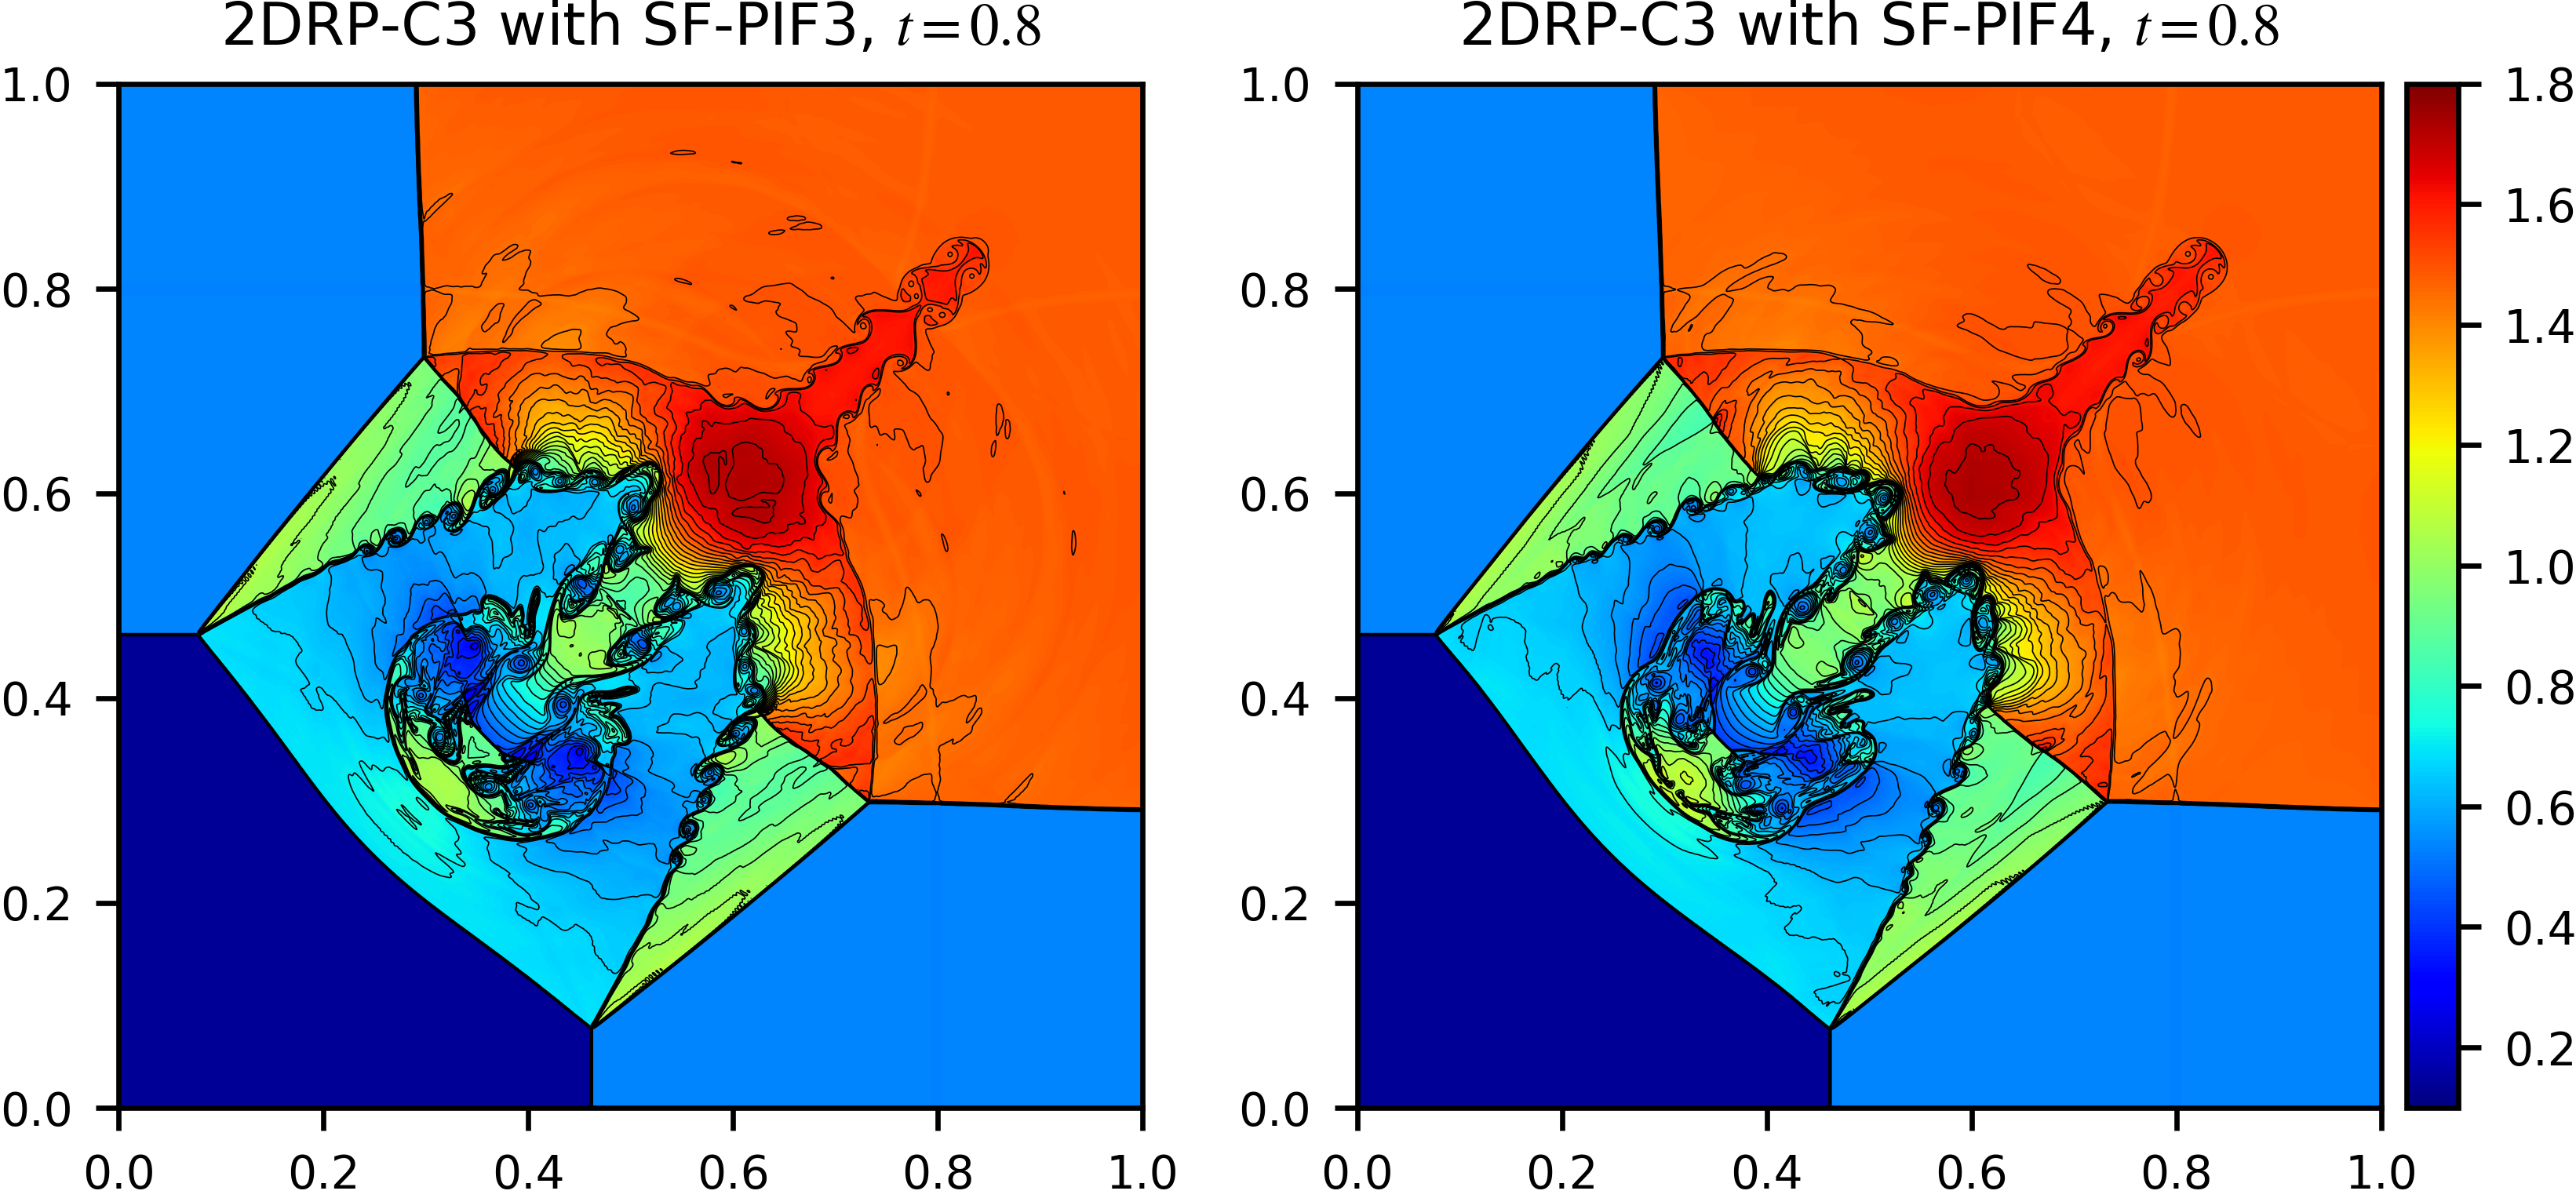
\includegraphics[width=0.9\textwidth]{fig/2drp_c3_weno5_sfPIF_1600.png}
    \end{subfigure}
    \caption{The density maps of Configuration 3 at \( t = 0.8 \).
        \textbf{Left column:} The solutions using RK3 (top) and SF-PIF3 (bottom).
        \textbf{Right column:} The solutions using RK4 (top) and SF-PIF4 (bottom).
        Forty levels of black contour lines are over-plotted in each figure
        with the same range of the color map.
        All simulations are performed on a \( 1600 \times 1600 \) grid resolution.
        }\label{fig:2drp_c3}
\end{figure}

The results at \( t = 0.8 \) are shown in~\cref{fig:2drp_c3}.
The pseudo-colors represent the density map ranging between \( [0.1, 1.8] \), and
40 contour lines within the same range are over-plotted as solid black lines.

As illustrated in the figures, all four different temporal schemes produce well-known,
acceptable results, keeping the assumed diagonal symmetry exceptionally well on this high resolution.
This problem is highly nonlinear, involving formations of the upward-moving jet,
the downward-moving mushroom-jet, secondary Kelvin-Helmholtz instabilities exhibited
as the small-scale vortical rollups along the slip lines and along the stems of the two jets.
Therefore, it is a non-trivial task to address if a method under consideration is
\textit{better} or \textit{worse} based on the number of such rollups in the simulations
without a systemic comparison analysis requiring extensive, careful validation and verification tests
that are beyond the scope of this dissertation.
At best, such quantification can only provide
proof of intrinsic information about the amount of numerical dissipation of each method.
From this perspective, one concludes that the two SF-PIF solutions produce
the equivalent amount of vortical rollups compared with the corresponding RK solutions,
although their different shapes on the downward jets,
confirming the validity of the recursive SF-PIF methods
on the presence of the shocks in 2D simulations.





\subsection{Double Mach reflection}\label{subsec:dmr_weno}

The double Mach reflection (DMR) test problem was firstly introduced by
Woodward and colella~\cite{woodward1984numerical}.
At initial, a planar shock is located at the left side of the domain
with a \( \ang{30} \) to the reflecting bottom surface.
As the shock propagates to the right, the bottom wall
continuously bounces off the shock wave and creates a round reflected shock.
The initial condition is the same as the original setup in~\cite{woodward1984numerical},
except for the doubled the \( y \)-domain size following~\cite{kemm2016proper}
to prevent numerical artifacts from the top boundary interaction with the
secondary shock wave and the slip line.

\begin{figure}
    \centering
    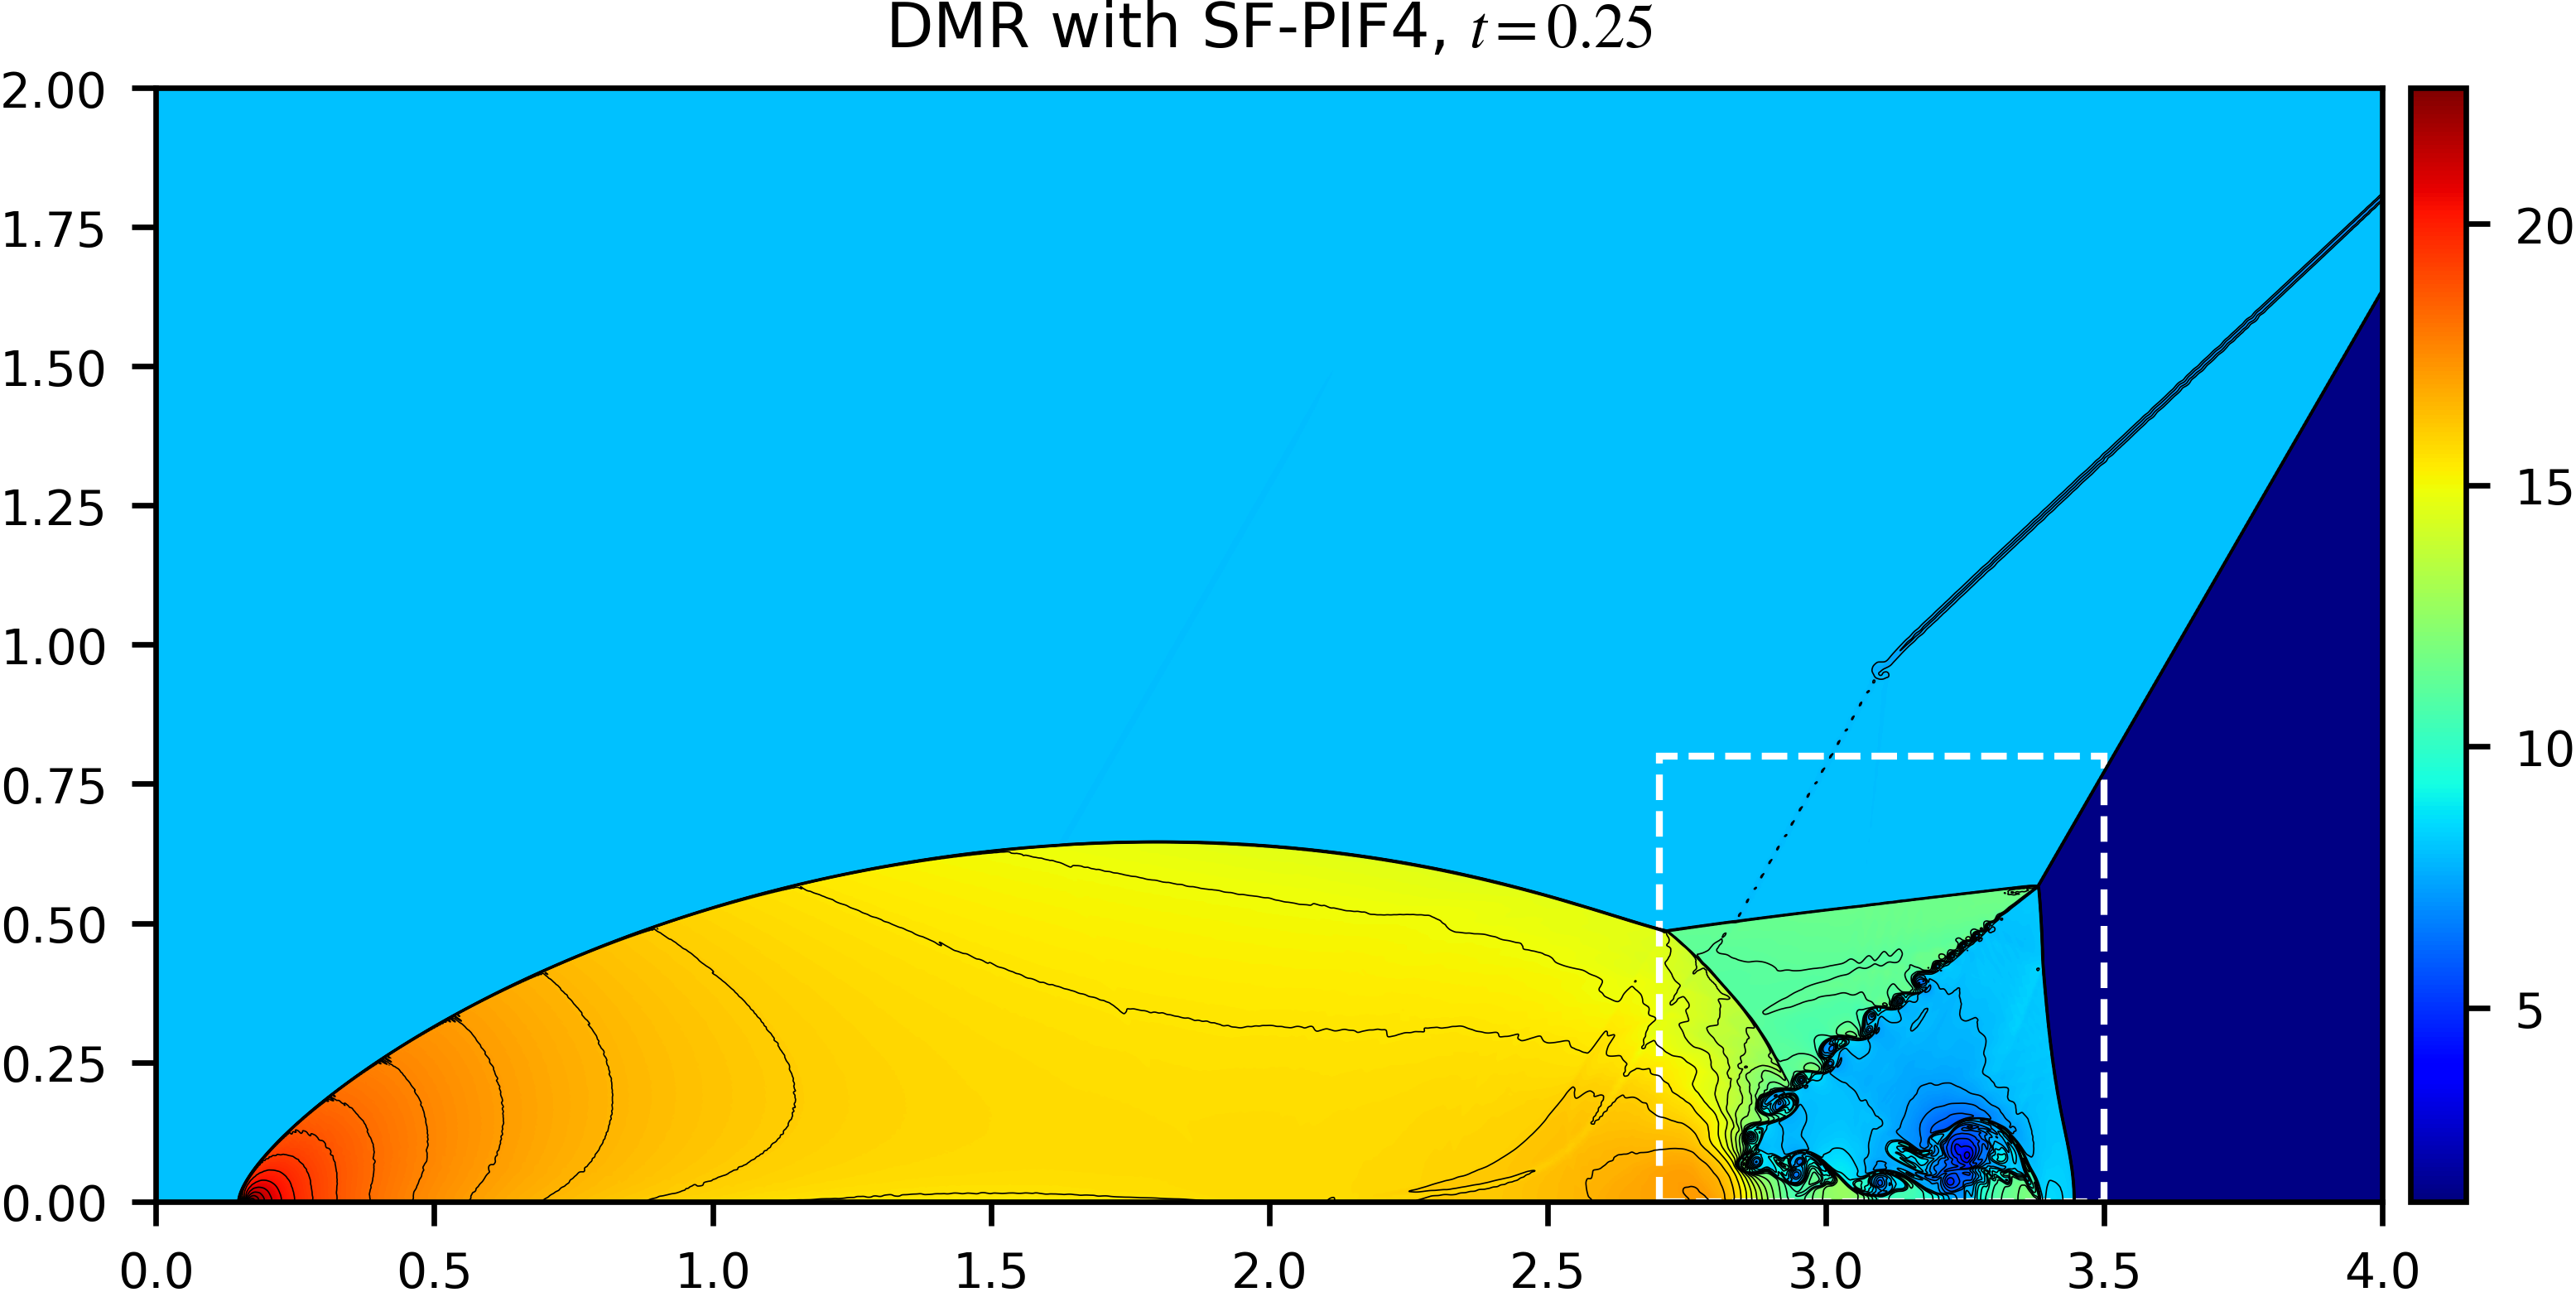
\includegraphics[width=0.85\textwidth]{fig/dmr_overview_sf4.png}
    \caption{The solution density profile of Double Mach reflection test
        solved with SF-PIF4 method on a \( 4096 \times 2048 \) grid resolution.
        The solid black curves represent the forty levels of contour lines
        ranging within the same range of the colormap.
        The white-dotted rectangle is the
        main point of interest in this simulation,
        where the jet and the primary triple point are formed.
        More detailed view of the rectangle region
        with different temporal solvers are plotted in~\cref{fig:dmr}.
    }\label{fig:dmr_overview}
\end{figure}

As the solution evolves, two contact discontinuities and two Mach stems are formed,
as well as a jet along the bottom surface. The formation of the jet is similar
to the formation of the two jets in implosion test (\cref{subsec:implosion}),
the collision of which led to the upward moving diagonal jet.
The solution density profiles resolved with the SF-PIF4 method
is portrayed in~\cref{fig:dmr_overview}.

\begin{figure}
    \centering
    \begin{subfigure}{140mm}
        \centering
        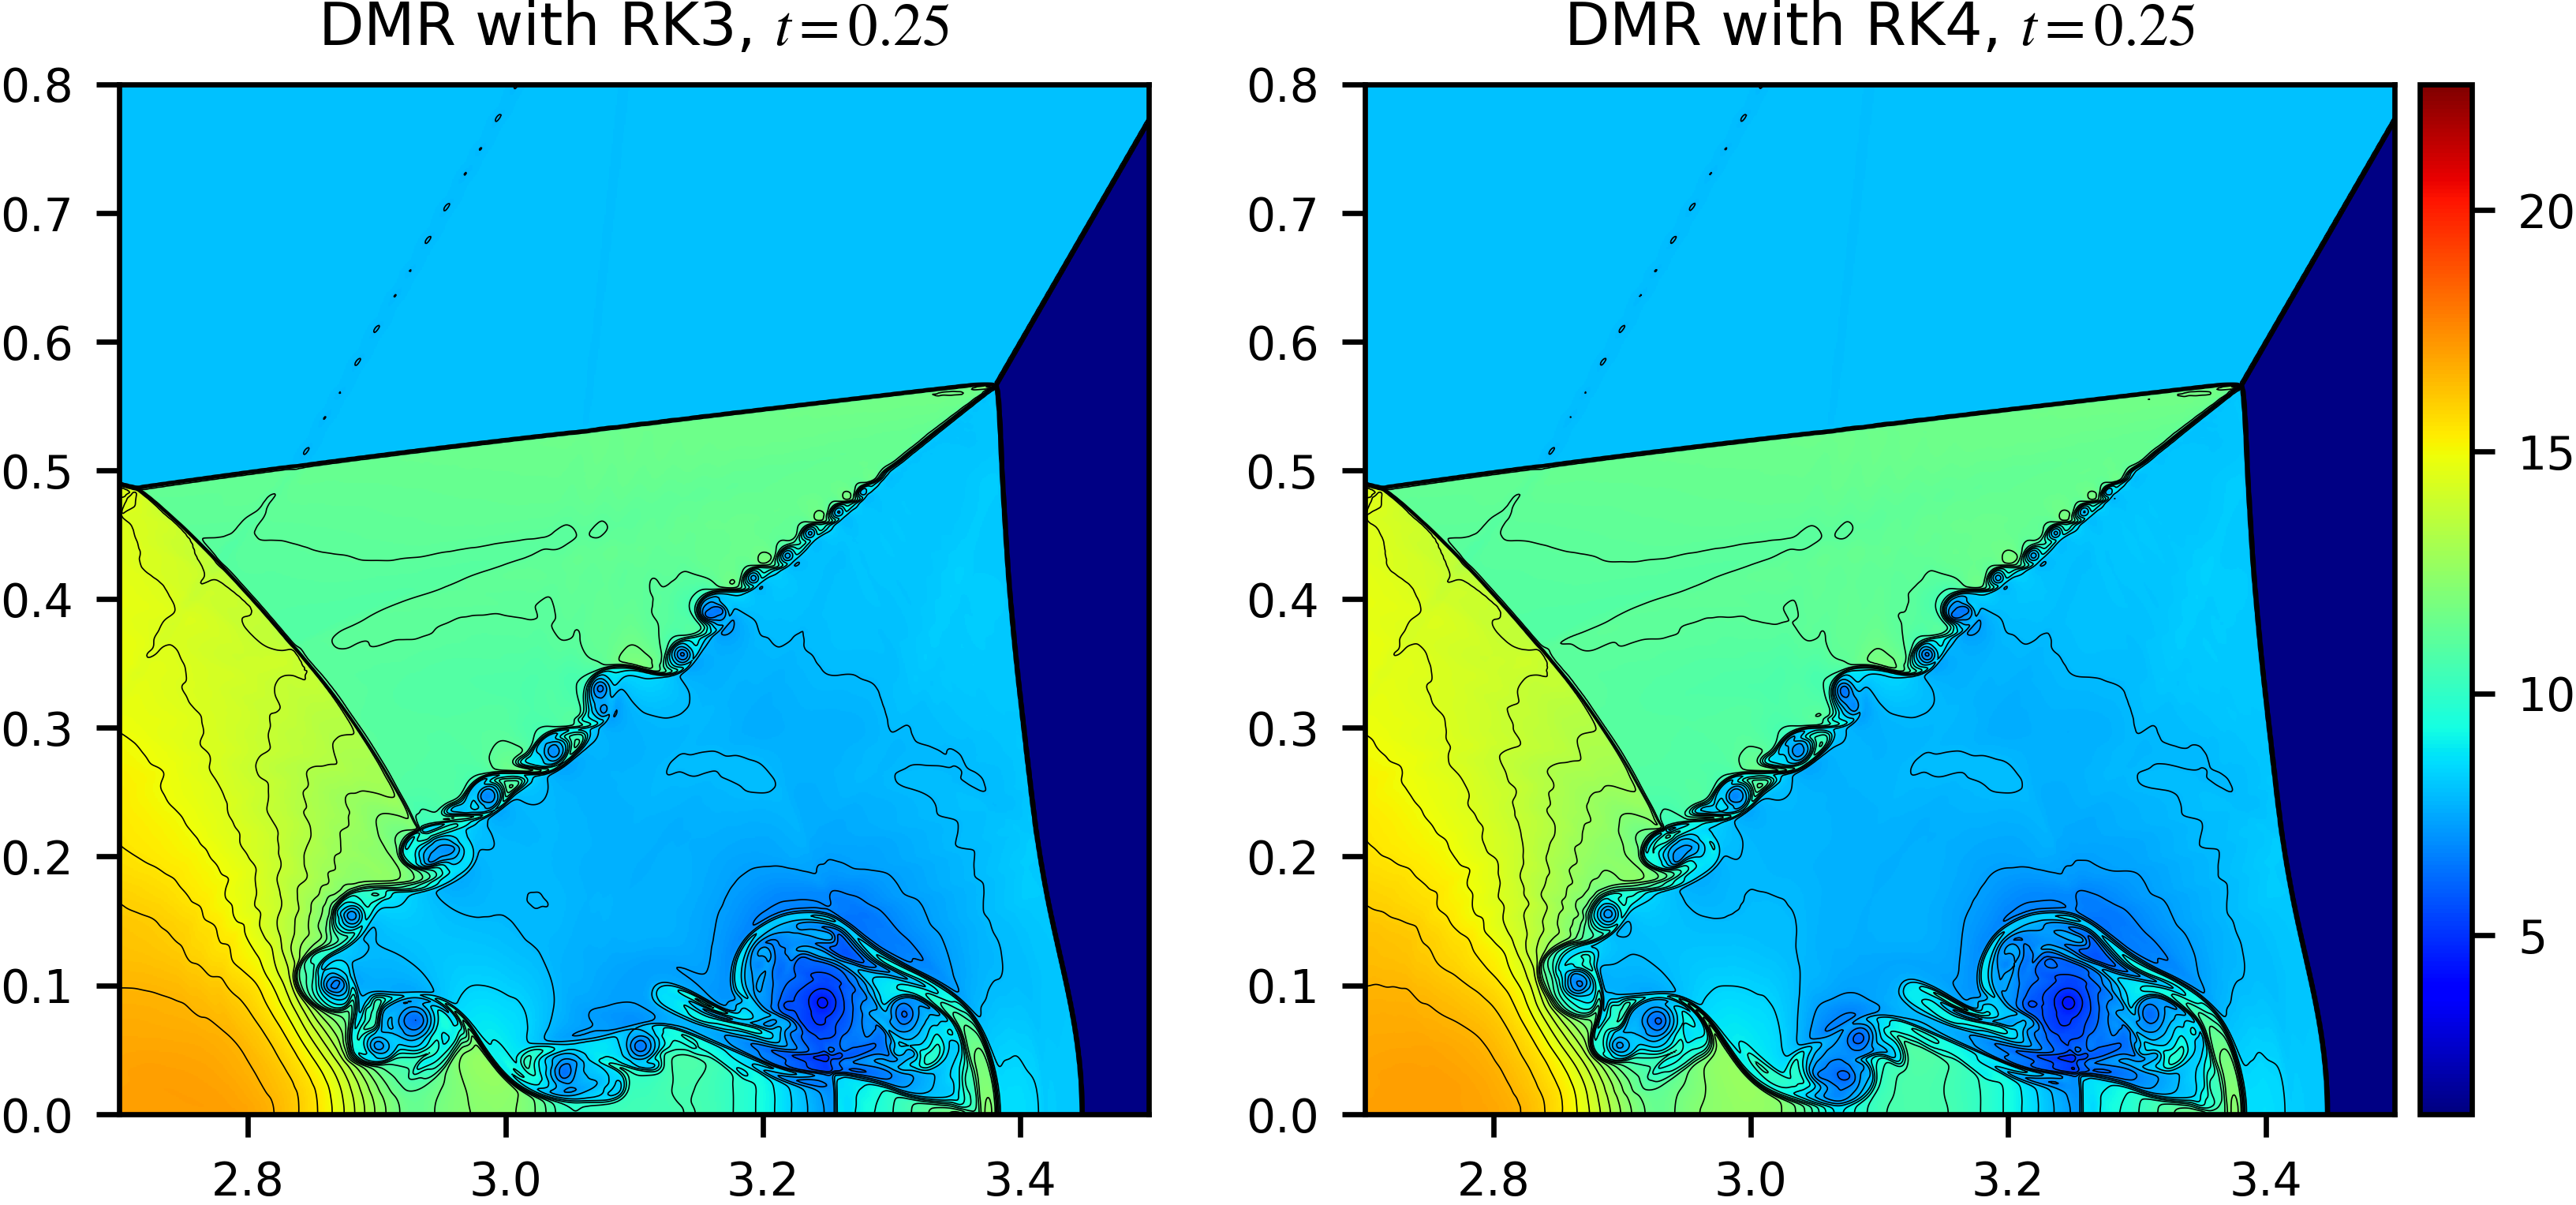
\includegraphics[width=0.95\textwidth]{fig/dmr_weno5_rk_4096y2.png}
    \end{subfigure}
    \begin{subfigure}{140mm}
        \centering
        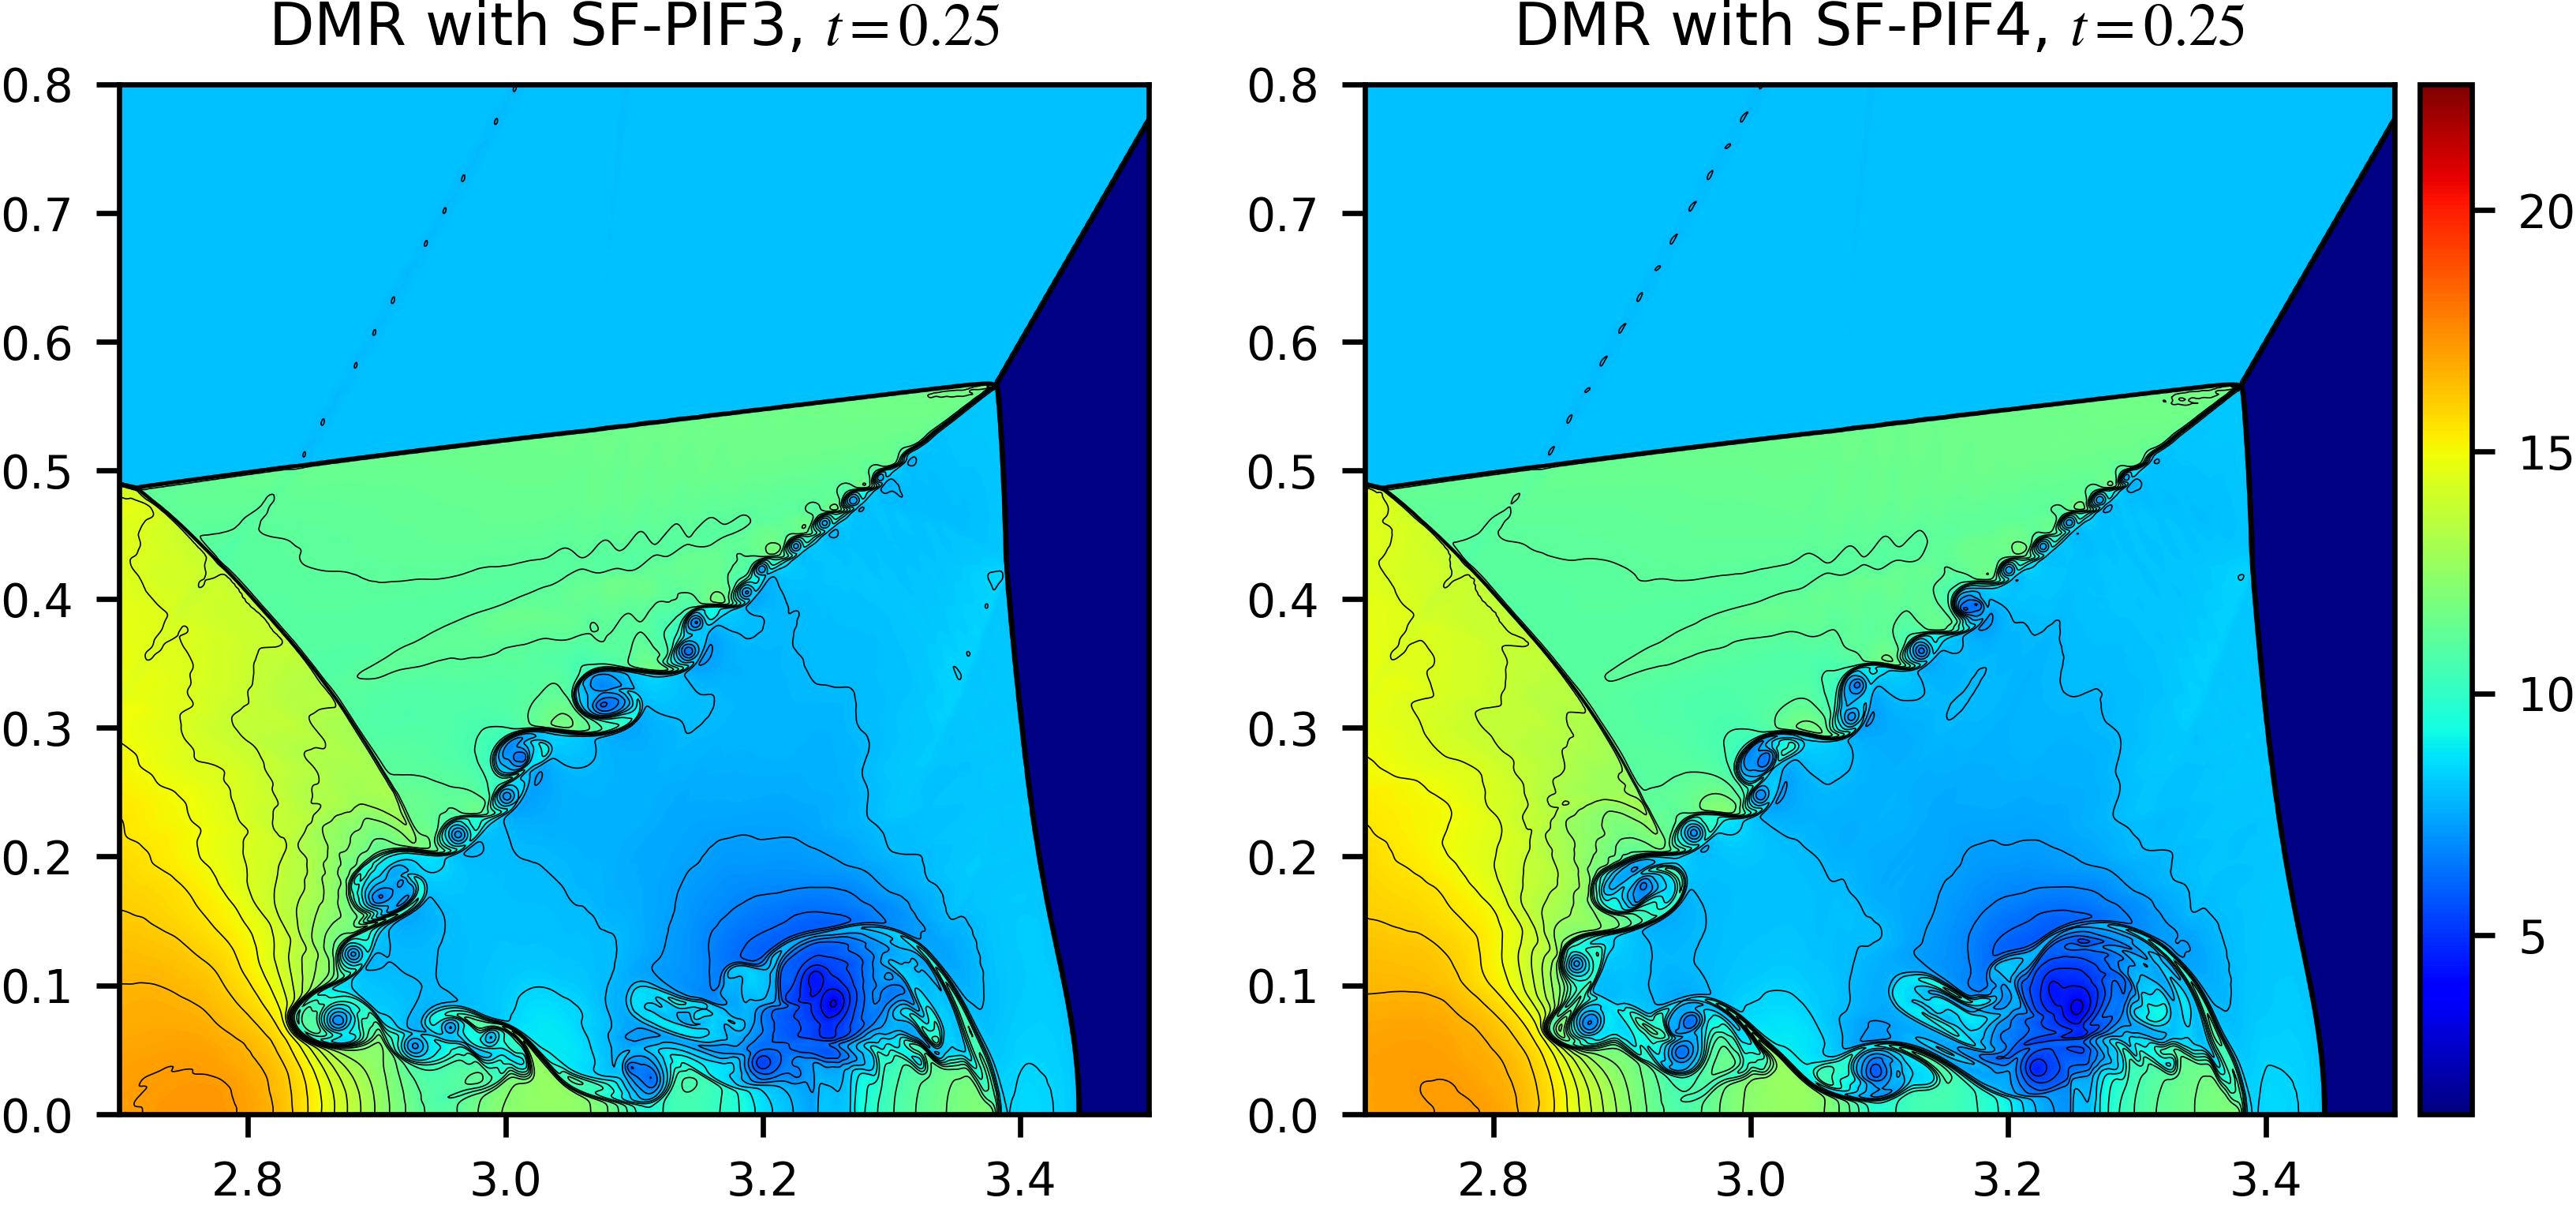
\includegraphics[width=0.95\textwidth]{fig/dmr_weno5_sf_4096y2.png}
    \end{subfigure}
    \caption{The density map of the double Mach reflection test at \( t = 0.25 \)
        zoomed-in near the jet. Forty levels of contour lines are over-plotted
        in solid black curves with the same range of the color map.
        All simulation results are performed on a
        \( 4096 \times 2048 \) grid resolution.
        \textbf{Left column:} The solutions using RK3 (top) and SF-PIF3 (bottom).
        \textbf{Right column:} The solutions using  RK4 (top) and SF-PIF4 (bottom).
    }\label{fig:dmr}
\end{figure}

\cref{fig:dmr} shows the zoomed-in views of the main point of interest in the DMR problem,
the vicinity of the jet and the primary triple point, resolved with four different temporal solvers.
Again, the results from the third- and fourth-order SF-PIF methods
produce well-acceptable results compared to the corresponding RK methods.
There are minor differences in the shape of Kelvin-Helmholtz instabilities along the
primary slip line and the bottom jet,
but the overall dynamics of the two SF-PIF solutions match well with the RK solutions,
validating the fidelity of the proposed SF-PIF methods in the presence of a strong shock.



\subsection{3D Riemann problem}\label{subsec:3drp}

The 3D Riemann problem is the 3D extension of the 2D Riemann problem described in~\cref{subsec:2drp_c3_weno},
introduced by Balsara~\cite{balsara2015three}.
Initially, each octant of the computational domain,
\( [-1, 1] \times [-1, 1] \times [-1, 1]\),
has constant initial conditions,
each of which will carry out 2D Riemann problem
including the diagonal plane of the 3D computational cubic.

\begin{figure}
    \centering
    \begin{subfigure}{140mm}
        \centering
        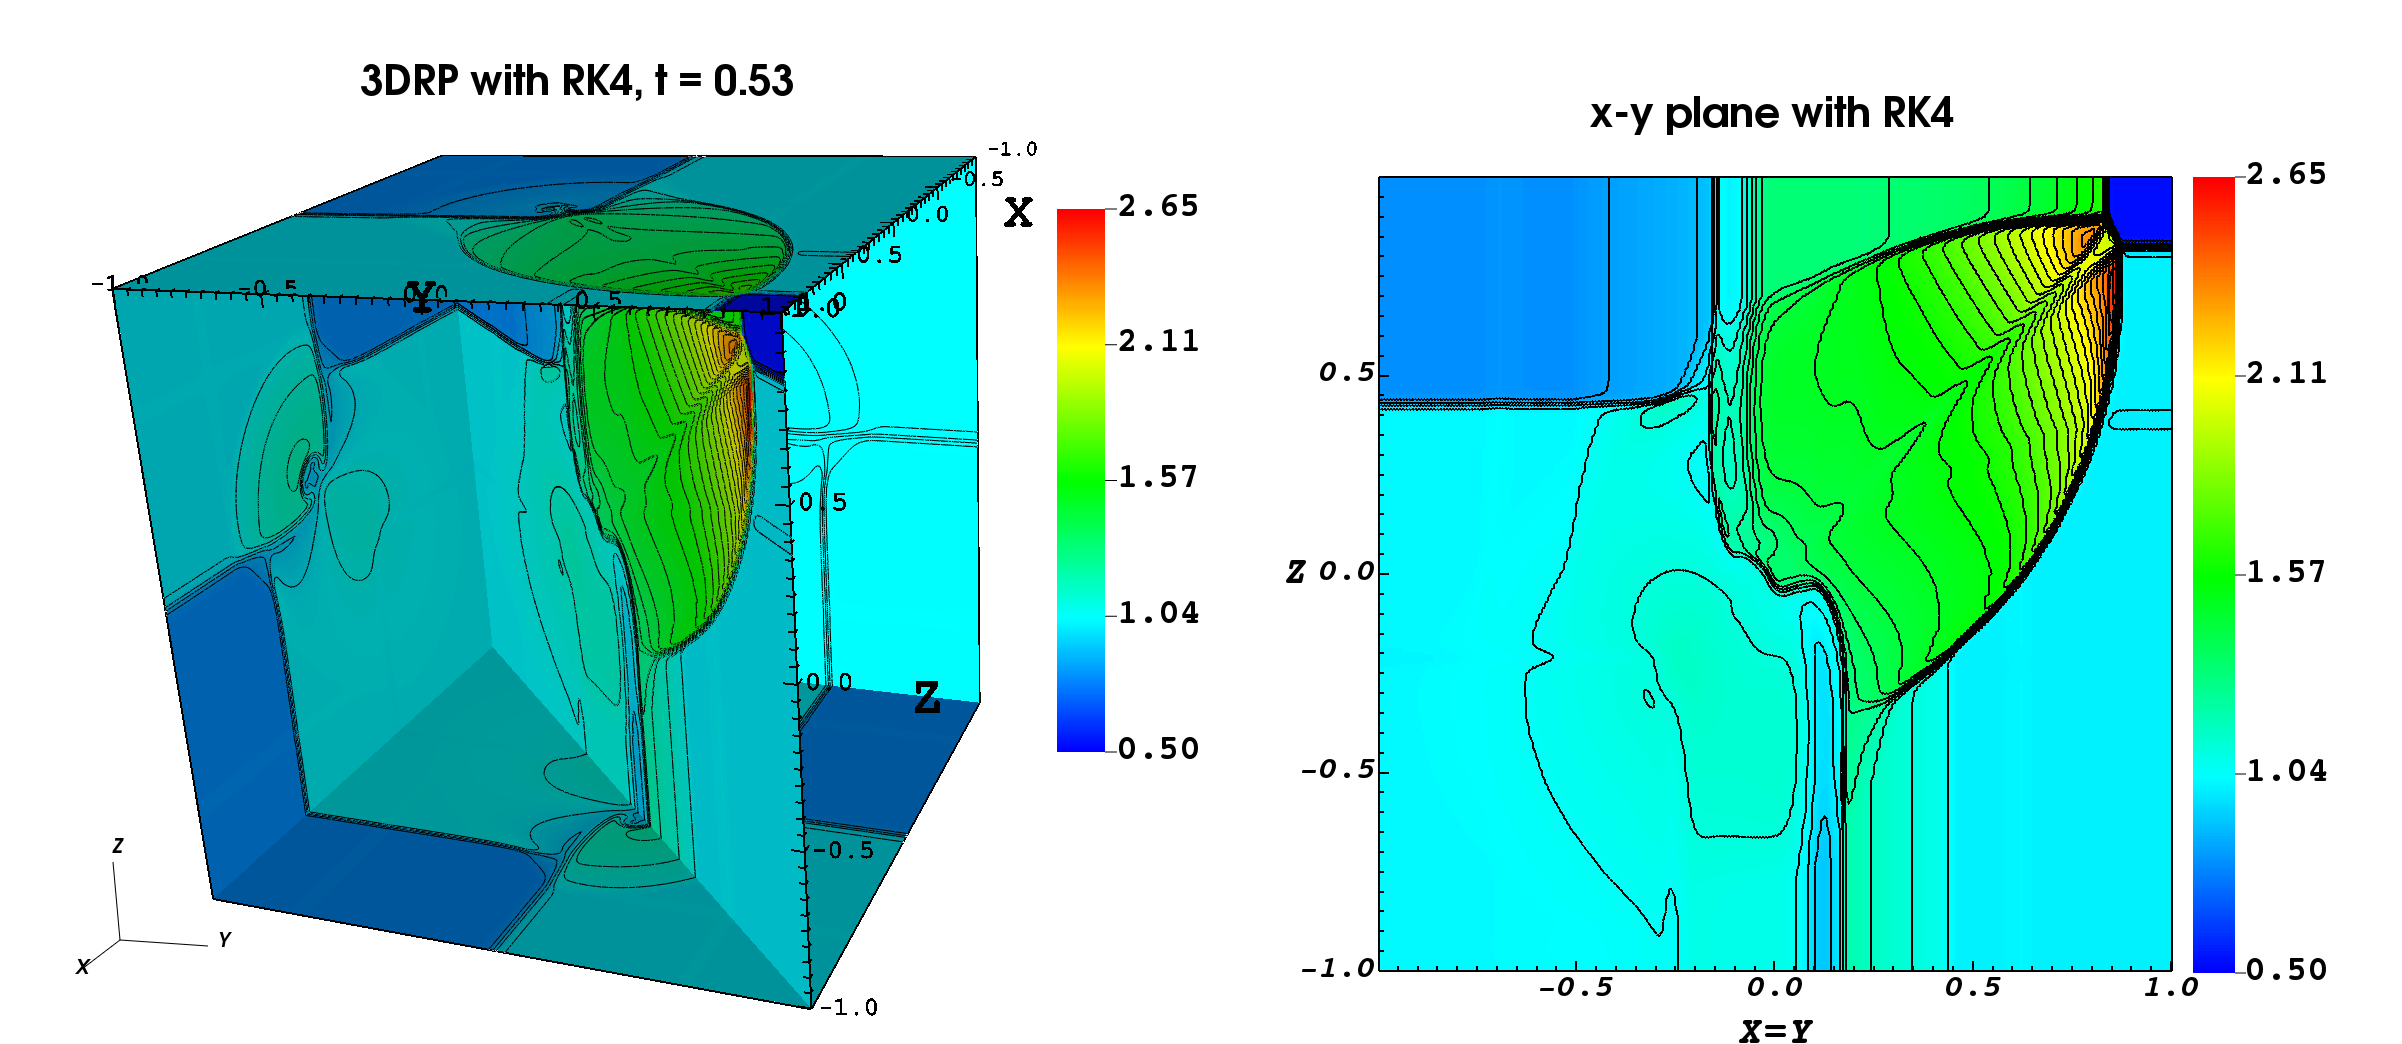
\includegraphics[width=0.95\textwidth]{fig/3drp_all_rk4.png}
    \end{subfigure}
    \begin{subfigure}{140mm}
        \centering
        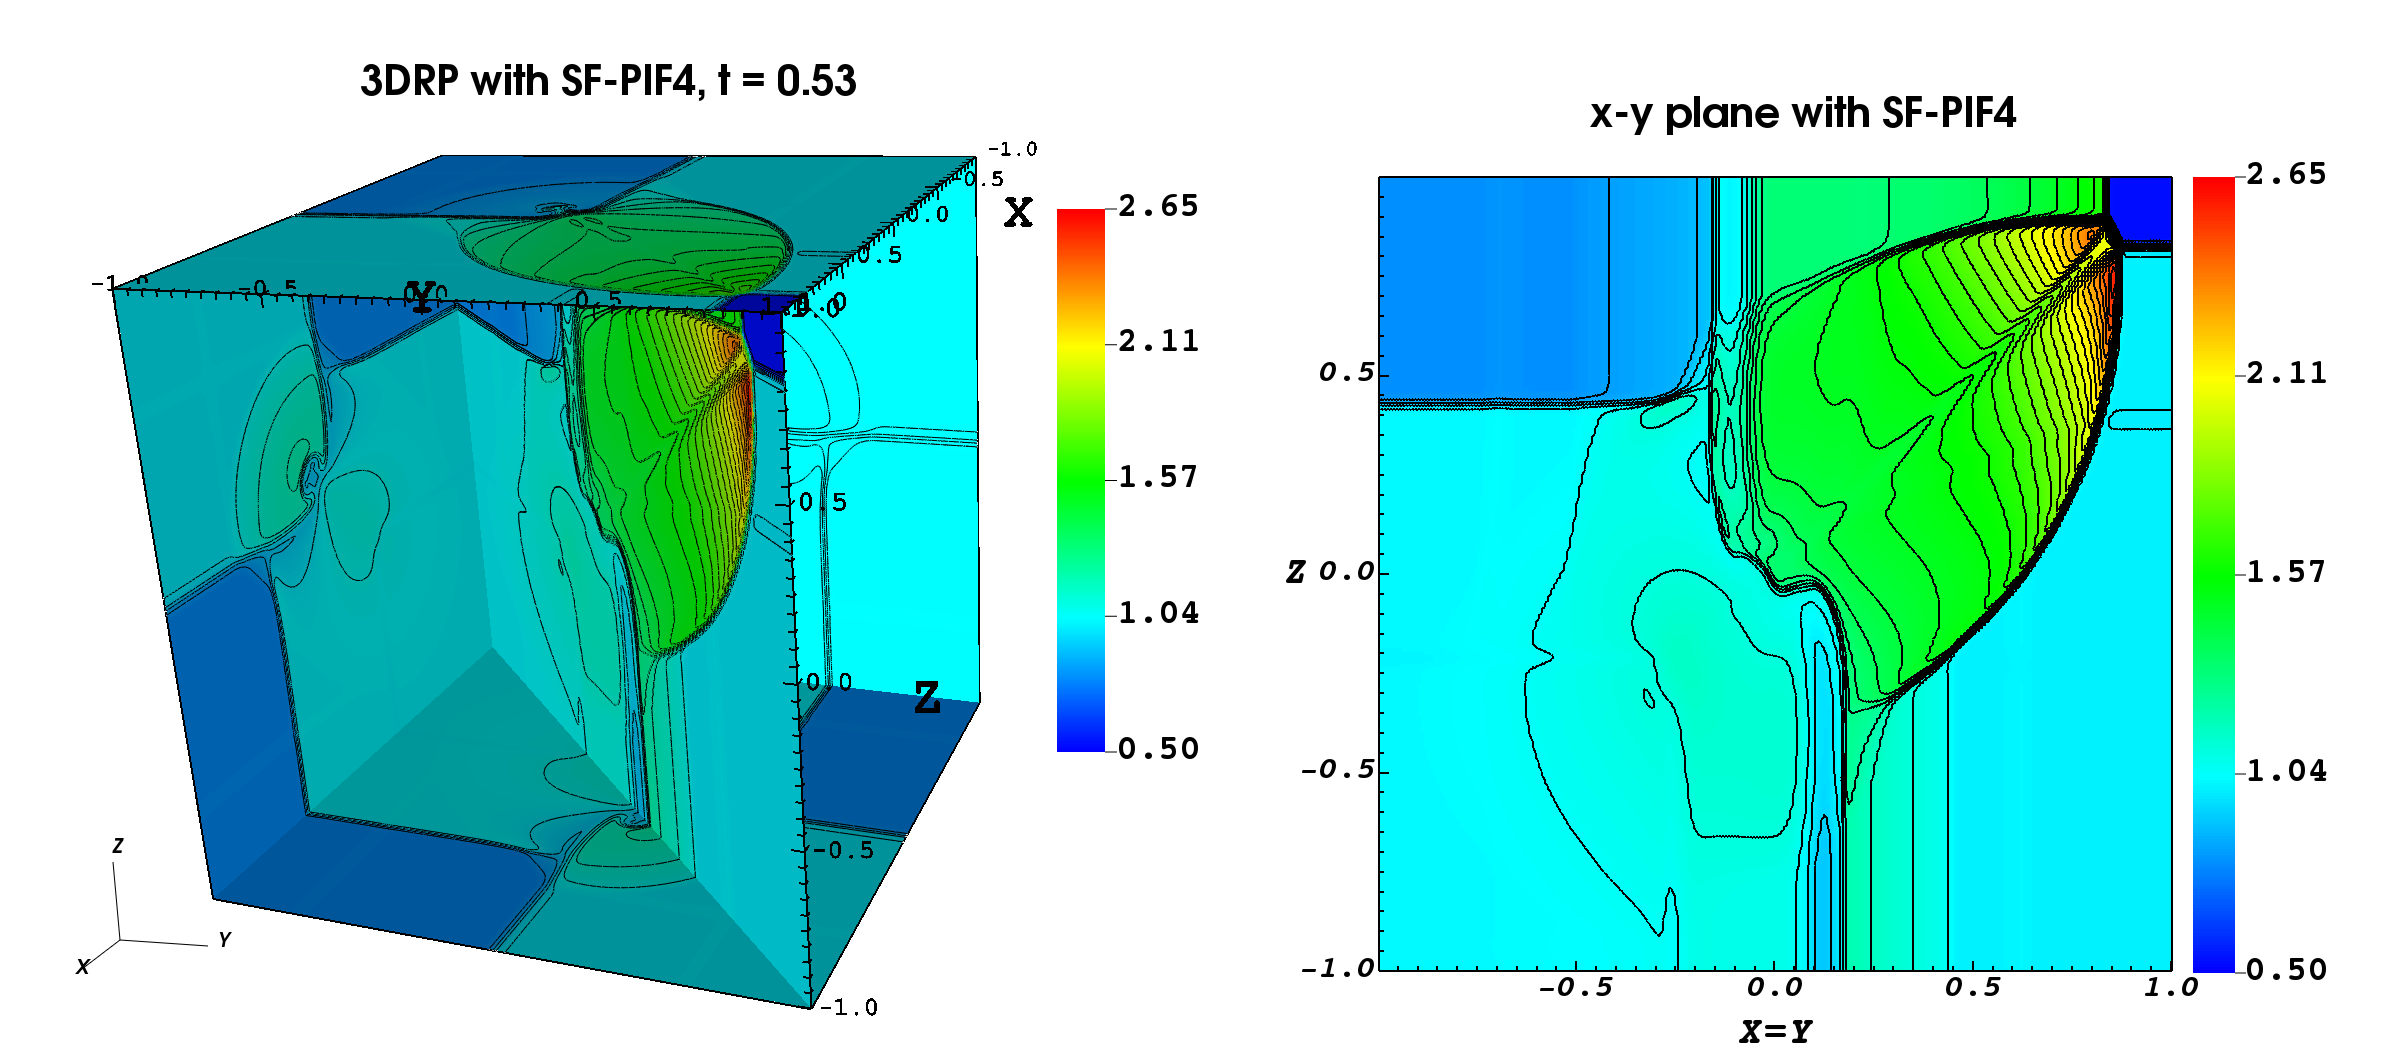
\includegraphics[width=0.95\textwidth]{fig/3drp_all_sf4.png}
    \end{subfigure}
    \caption{The density maps of the 3D Riemann problem test at \( t = 0.53 \).
        Forty contour lines are over-plotted.
        The left panels show each face's geometrical views, while 
        the right panels show
        the detailed picture of the diagonal planes.
        All simulations are performed on a \( 256 \times 256 \times 256 \) grid resolution,
        solved with RK4 (\textbf{top}) and SF-PIF4 (\textbf{bottom}) solvers.
        The Courant condition, \( C_{\text{cfl}} = 0.3 \) is used for
        calculating the timestep.
    }\label{fig:3drp}
\end{figure}

The results of 3D Riemann problem solved with RK4 and SF-PIF4 are
illustrated in~\cref{fig:3drp}. The solutions were resolved on a
\( 256 \times 256 \times 256 \) grid resolution.
The pseudo-color map ranges between \( [0.5, 2.65] \),
and 40 levels of contour lines are over-plotted using the same range.
As depicted in~\cref{fig:3drp}, each surface of 3D computational domain
evolves different 2D Riemann problems, including the diagonal plane which is
separately plotted on the left panel.
The recursive SF-PIF4 method is able to capture all the important features as much as the RK4 result,
confirming the validity of the SF-PIF4 method in 3D simulation with strong shocks.

\begin{table}
    \centering
    \caption{Performance results for the 3DRP test problem.
        All performance results (measured in seconds) are averaged over
        five simulation runs conducted on 16 nodes.% of \textit{lux} cluster.
        Each node has 2 \( \times \) 20-core Intel Xeon Gold 6248 (Cascade Lake) CPUs,
        and the simulation utilized 512 parallel threads for each run.
    }\label{table:3drp}
    \begin{adjustbox}{width=\textwidth}
        \begin{tabular}{@{}cccccccccccc@{}}
            \toprule
            \multirow{2}{*}{Grid Resolution} & \multicolumn{2}{l}{RK3} &  & \multicolumn{2}{l}{SF-PIF3}
                    & & \multicolumn{2}{l}{RK4} & & \multicolumn{2}{l}{SF-PIF4} \\
            \cmidrule(lr){2-3} \cmidrule(l){5-6} \cmidrule(l){8-9} \cmidrule(l){11-12}
            & CPU Time & Speedup &  & CPU Time & Speedup & & CPU Time & Speedup & & CPU Time & Speedup\\
            \midrule
            \( 64 \times 64 \times 64 \)   & \SI{1.79}{\second} & 1.0 &  & \SI{1.09}{\second} & 0.61 & &
                \SI{2.95}{\second} & 1.64 &  & \SI{2.67}{\second} & 1.49 \\
            \( 128 \times 128 \times 128 \) & \SI{15.62}{\second} & 1.0 &  & \SI{7.63}{\second} & 0.49 & &
                \SI{25.88}{\second} & 1.66 &  & \SI{18.97}{\second} & 1.21 \\
            \( 256 \times 256 \times 256 \) & \SI{191.00}{\second}   & 1.0 &  & \SI{82.02}{\second} & 0.43 & &
                \SI{321.34}{\second} & 1.68 &  & \SI{201.40}{\second} & 1.05 \\
            \( 512 \times 512 \times 512 \) & \SI{2679.85}{\second}  & 1.0 &  & \SI{1173.54}{\second} & 0.44 & &
                \SI{4507.88}{\second} & 1.68 &  & \SI{2817.78}{\second} & 1.05 \\
        \end{tabular}
    \end{adjustbox}
\end{table}

\cref{table:3drp} shows the performance results for the 3D Riemann problem test
on four grid resolutions.
As shown in the table, the SF-PIF4 method demonstrates nearly the same performance
as the \textit{third}-order RK method, especially in high-resolution cases.
It is important to note that the performance gains from the SF-PIF methods
are more compensated on the high-resolution grids,
which are indispensable for high fidelity physical simulation studies.

\section{SF-PIF method with GP-WENO}\label{sec:result_gpweno}

As mentioned in~\cref{chap:sfpif}, the SF-PIF method is an entirely independent temporal solver,
which does not require any modification in the spatial high-order part of the simulation codes
alike RK methods.
As the purpose of demonstrating the portability of the SF-PIF method,
this section will conduct several test problems using GP-WENO
(instead of the conventional WENO as in the previous sections) described in~\cref{subsec:gp}
as a spatial high-order reconstruction method
combining with SF-PIF methods for time integration strategy.

\subsection{Hyperparameters}\label{subsec:hyper_params_gpweno}

Unlike the polynomial-based reconstruction schemes,
the GP method lacks any analytical considerations of the behavior of numerical errors
with respect to the grid resolutions.
This is further complicated by the use of nonlinear weighting in the GP-WENO method,
which is necessary to capture the discontinuities appropriately.
Consequently, direct numerical experiments
should be conducted to predict the numerical errors from the GP-WENO method.

The GP-WENO method has two hyperparameters that need to be tuned,
the length hyperparameter \( \ell \)
and the shock-capturing hyperparameter \( \sigma \).
The numerical errors from the 2D vortex advection problem
with varying hyperparameters are illustrated in~\cref{fig:gp_hp_cmap}.
The simulations are conducted on \( 400 \times 400 \) grid resolutions,
resolved with SF-PIF3 temporal solver
with the same setup in~\cref{subsec:vortex_weno}.
As dotted white lines represent,
the minimum error has been found with \( \ell = \sigma = 1\)
for this systematic test.

\begin{figure}
    \centering
    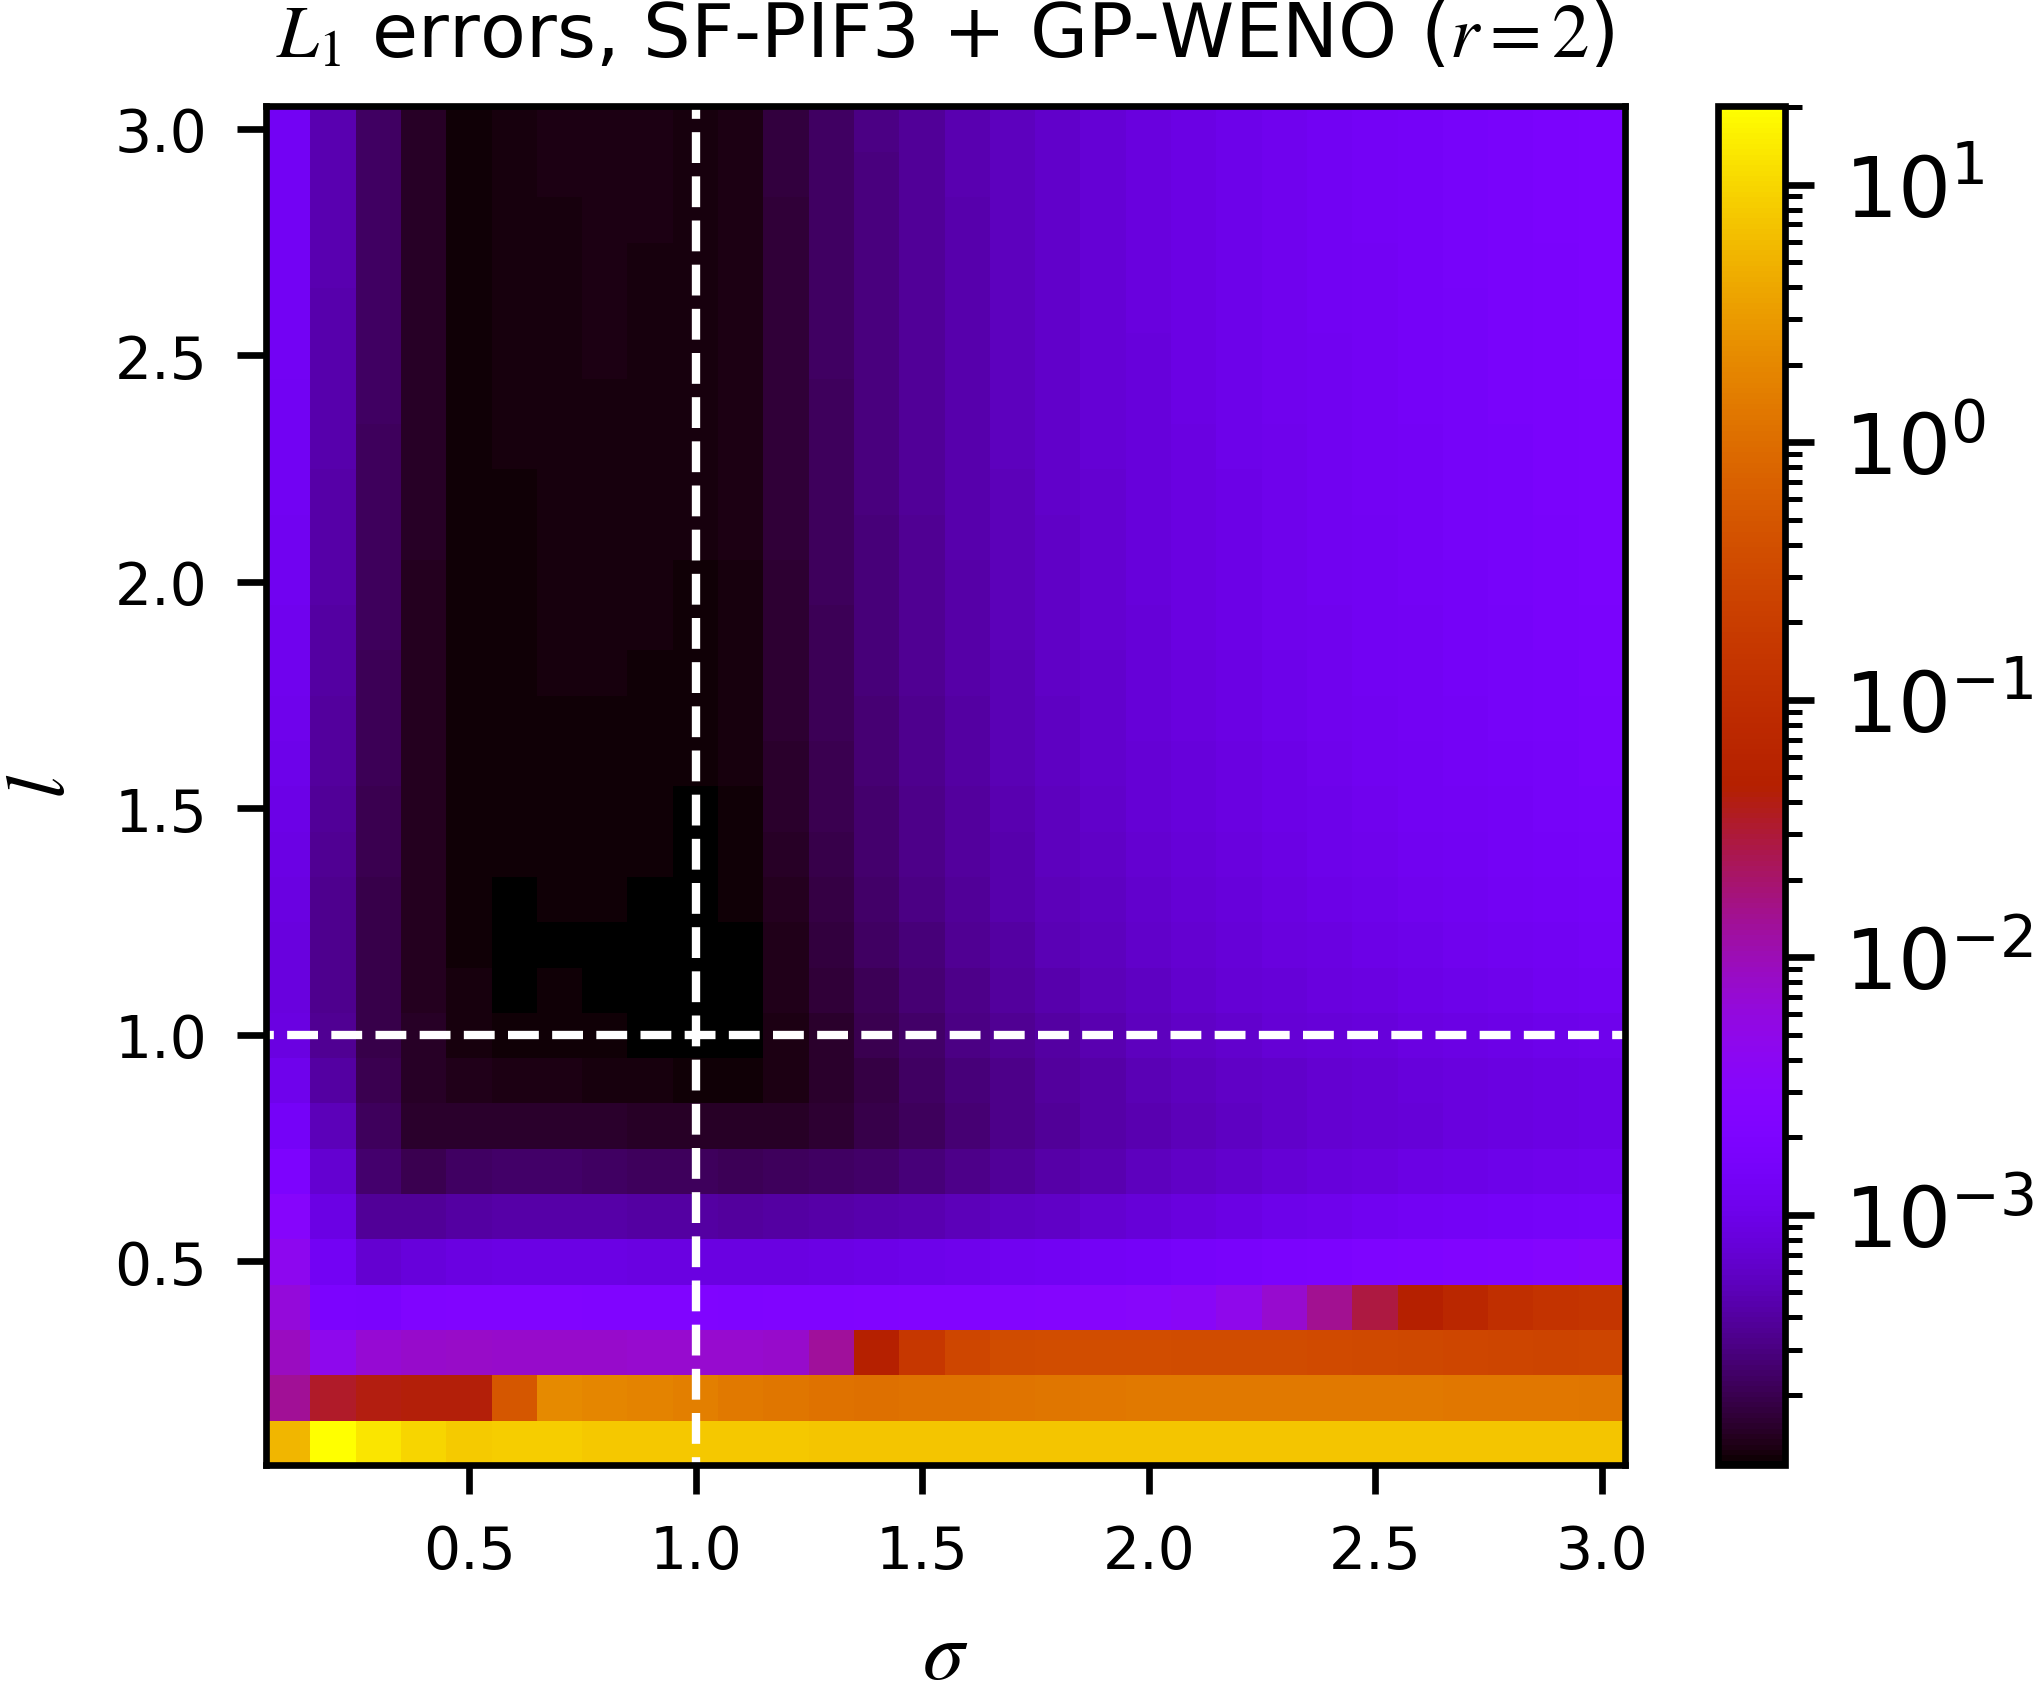
\includegraphics[width=0.85\textwidth]{fig/hp_cmap_gp2_sf3.png}
    \caption{The \( L_{1} \) errors of vortex advection problem solved by
        GP-WENO and SF-PIF3 on a \( 400 \times 400 \) grid resolution.
        The radius of GP-WENO stencil is \( r=2 \), which is the same
        stencil size of the fifth-order WENO method.
        Using other temporal solvers produces the same pattern,
        and omitted in this study.
        The white dotted-lines are represent the
        hyperparameters of minimum error.
    }\label{fig:gp_hp_cmap}
\end{figure}

\begin{figure}
    \centering
    \begin{subfigure}{70mm}
        \centering
        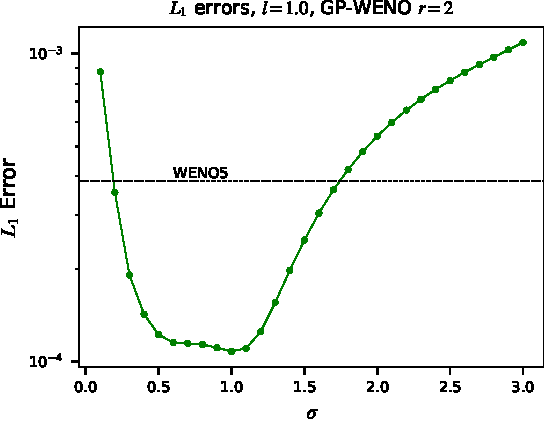
\includegraphics[width=0.95\textwidth]{fig/hp_best_ell_gp2_sf3}
    \end{subfigure}
    \begin{subfigure}{70mm}
        \centering
        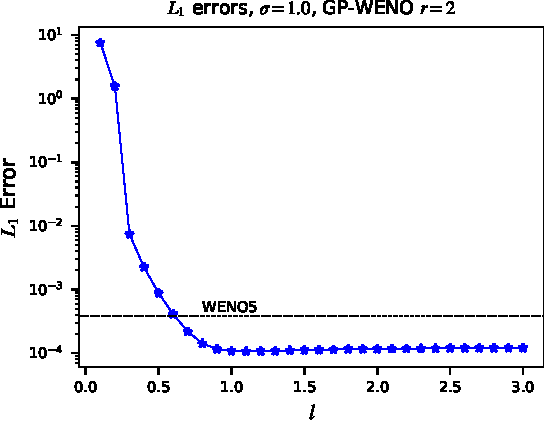
\includegraphics[width=0.95\textwidth]{fig/hp_best_sig_gp2_sf3}
    \end{subfigure}
    \caption{The slices of~\cref{fig:gp_hp_cmap} at the minimum error.
        The horizontal dotted line is the target error obtained from WENO method
        with same configurations.
    }\label{fig:gp_hp_best}
\end{figure}

\cref{fig:gp_hp_best} shows the slice plots by following the dotted lines
in~\cref{fig:gp_hp_cmap}, showing the \( L_{1} \) errors
with the best choice of \( \ell \) and \( \sigma \).
Surprisingly, the shock-capturing hyperparameter \( \sigma \) affects the solution accuracy,
even though the solution is entirely smooth.
Theoretically speaking, the vortex advection test is a nonlinear smooth problem,
and \( \sigma \) only plays a role in the presence of a shock discontinuity;
thus, it has to have the same errors across all sigma values.
The different errors with varying sigma in the smooth problem are the indication
of numerical errors in calculating nonlinear weights of GP-WENO\@.
This could be arisen from calculating the linear weights,
(i.e., solving the overdetermined system~\cref{eq:gp_weno_overdetermined_matrix})
or calculating smoothness indicators in~\cref{eq:gp_smoothness_ind},
which requires further studies.
Nonetheless, since the numerical solvers are involved in calculating
both the linear weights and smoothness indicators,
e.g., the least square method and QR algorithm,
numerical errors are inevitable in GP-WENO nonlinear weights.

Notwithstanding the fact that the GP-WENO method with \( \sigma = 1 \)
has the smallest amount of \( L_{1} \) errors
from the previous tests, however,
another numerical tests argue that the large \( \sigma \) values
degrade the solution accuracy in high-resolution simulation.

\begin{figure}
    \centering
    \begin{subfigure}{70mm}
        \centering
        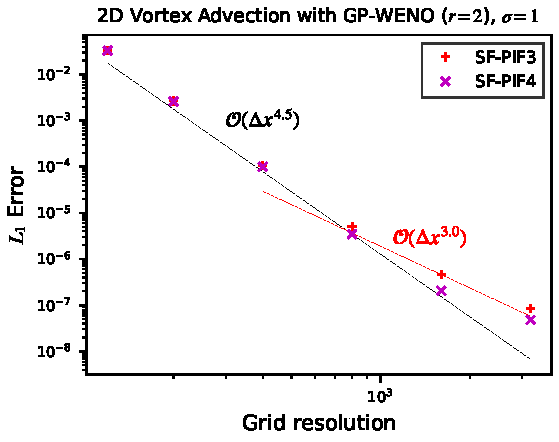
\includegraphics[width=0.95\textwidth]{fig/gp2_vortex_error_sigma1}
    \end{subfigure}
    \begin{subfigure}{70mm}
        \centering
        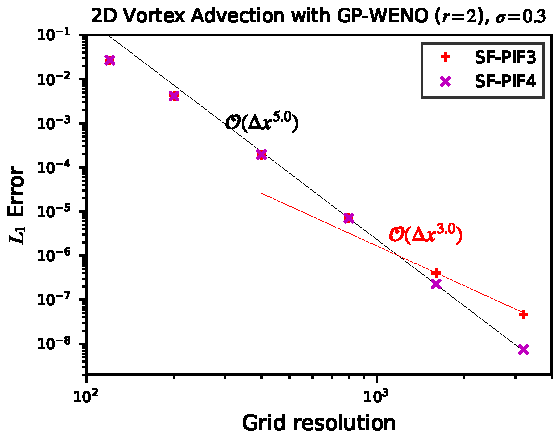
\includegraphics[width=0.95\textwidth]{fig/gp2_vortex_error_sigma03}
    \end{subfigure}
    \caption{The convergence rate of GP-WENO method with \( r=2 \) obtained by solving
        2D isentropic vortex advection problem on varying grid resolutions.
        Two temporal methods, SF-PIF3 and SF-PIF4 are used for integrating the solution,
        and the behavior of third-order and fourth-order temporal schemes
        is identical to the results from~\cref{subsec:vortex_weno}.
        The GP length hyperparameters, \( \ell = 1 \) is used for both tests,
        and the shock-capturing hyperparameter
        \textbf{Left:} \( \sigma = 1 \), and \textbf{Right:} \( \sigma = 0.3 \)
        are used.
        The tests with \( \sigma = 1 \) on the left panel have smaller absolute \( L_{1} \) error,
        but failed to maintaining the convergence rate on high-resolution grids.
        On the other hand, tests with \( \sigma = 0.3 \) demonstrate consistent
        convergence rate on all grid configurations.
    }\label{fig:gp_vortex_convergence}
\end{figure}

\cref{fig:gp_vortex_convergence} shows that the GP-WENO method's hyperparameter \( \sigma \)
affects the convergence rate significantly.
As shown in the left panel of~\cref{fig:gp_vortex_convergence},
the GP-WENO method with the choice of \( \sigma = 1 \) can not retain
the expected order of convergence rate
in high-resolution regimes
both with SF-PIF3 and SF-PIF4 methods.
On the other hand, the choice of \( \sigma = 0.3 \) on the right panel of~\cref{fig:gp_vortex_convergence}
shows similar performance results as in the discussions of~\cref{subsec:vortex_weno},
although the absolute magnitudes of \( L_{1} \) errors are slightly larger than
the case of \( \sigma = 1 \).

\begin{table}
    \centering
    \caption{The \( L_{1} \) errors, the rates of convergence,
        and the computation times for the vortex advection test
        solved using GP-WENO method with radius of \( r = 2 \).
        The hyperparameters, \( \ell = 1 \) and \( \sigma = 0.3 \)
        are used for all simulation based on the results of~\cref{fig:gp_vortex_convergence}.
        The ``Speedup'' columns represent the relative speed-ups
        compared to the WENO5 method with corresponding temporal solveers.
        All simulation runs are
        performed on the four 20-cores
        Cascade Lake Intel Xeon processors, utilized 64 parallel threads.
        CPU times are measured in seconds, averaged over 10 individual runs.
    }\label{table:vortex_gp2}
    \begin{adjustbox}{width=\textwidth}
        \begin{tabular}{@{}ccccclcccc@{}}
            \toprule
            \multirow{2}{*}{\( N_{x} = N_{y} \)} & \multicolumn{4}{c}{GP-WENO + SF-PIF3} &  & \multicolumn{4}{c}{GP-WENO + SF-PIF4} \\
            \cmidrule(lr){2-5} \cmidrule(l){7-10}
            & \(L_{1}\) error & \(L_{1}\) order & CPU Time & Speedup &  &
            \(L_{1}\) error & \(L_{1}\) order & CPU Time & Speedup \\ \midrule
            120  & \num{2.68E-2} & \--- & \SI{0.67}{\second}      & 0.95 &  & \num{2.67E-2} & \--- & \SI{1.36}{\second}     & 0.92 \\
            200  & \num{4.16E-3} & 3.65 & \SI{2.43}{\second}      & 0.88 &  & \num{4.17E-3} & 3.66 & \SI{4.97}{\second}     & 0.93 \\
            400  & \num{1.91E-4} & 4.44 & \SI{16.86}{\second}     & 0.85 &  & \num{1.94E-4} & 4.42 & \SI{33.39}{\second}    & 0.93 \\
            800  & \num{7.12E-5} & 4.75 & \SI{133.79}{\second}    & 0.87 &  & \num{7.07E-6} & 4.78 & \SI{252.08}{\second}   & 0.93 \\
            1600 & \num{4.05E-7} & 4.14 & \SI{1061.26}{\second}   & 0.88 &  & \num{2.28E-7} & 4.95 & \SI{1944.68}{\second}  & 0.93 \\
            3200 & \num{4.71E-8} & 3.10 & \SI{8375.05}{\second}   & 0.89 &  & \num{7.48E-9} & 4.93 & \SI{15514.25}{\second} & 0.95 \\
        \end{tabular}
    \end{adjustbox}
\end{table}

The detailed numerics of the GP-WENO's convergence tests are summarized in~\cref{table:vortex_gp2}.
The all simulation runs are performed with the same configurations of WENO5 tests in~\cref{table:vortex_weno_fourth};
thus, the ``Speedup'' columns portray the relative speed-ups of GP-WENO method
compared to the conventional fifth-order WENO method.
The GP-WENO method with appropriately selected hyperparameters
produces less \( L_{1} \) errors and better convergence rate
with the high-order temporal method, SF-PIF4.
On the other hand, the GP-WENO method coupled with the relatively low-order temporal solver, SF-PIF3,
experiences the convergence rate degradation more faster than the WENO5.







\subsection{Strong shock vortex interaction}\label{subsec:shock_vortex}

In order to test GP-WENO's numerical capability to capturing
a complex flow patterns with both smooth regions and discontinuous shock waves,
the strong shock vortex interaction test~\cite{cheng2019two,galbraith5th} is considered.
Initially, a Mach 1.5 stationary shock is present at \( x = 0.5 \),
and the vortex is located at the center of \( (x_{c}, y_{c}) = (0.25, 0.5) \).
As the simulation evolves, the vortex moves with the background flow,
which is traveling toward to a stationary shock.
Consequently, the vortex penetrates the stationary shock,
evolving complex fluid structures of the ``squeezed'' vortex.
The computational domain is a 2D rectangle box of \( [0,2]\times[0,1] \)
with an inflow boundary on the left and an outflow boundary on the right.
Bottom and top boundaries are reflected walls.

\begin{figure}
    \centering
    \begin{subfigure}{120mm}
        \centering
        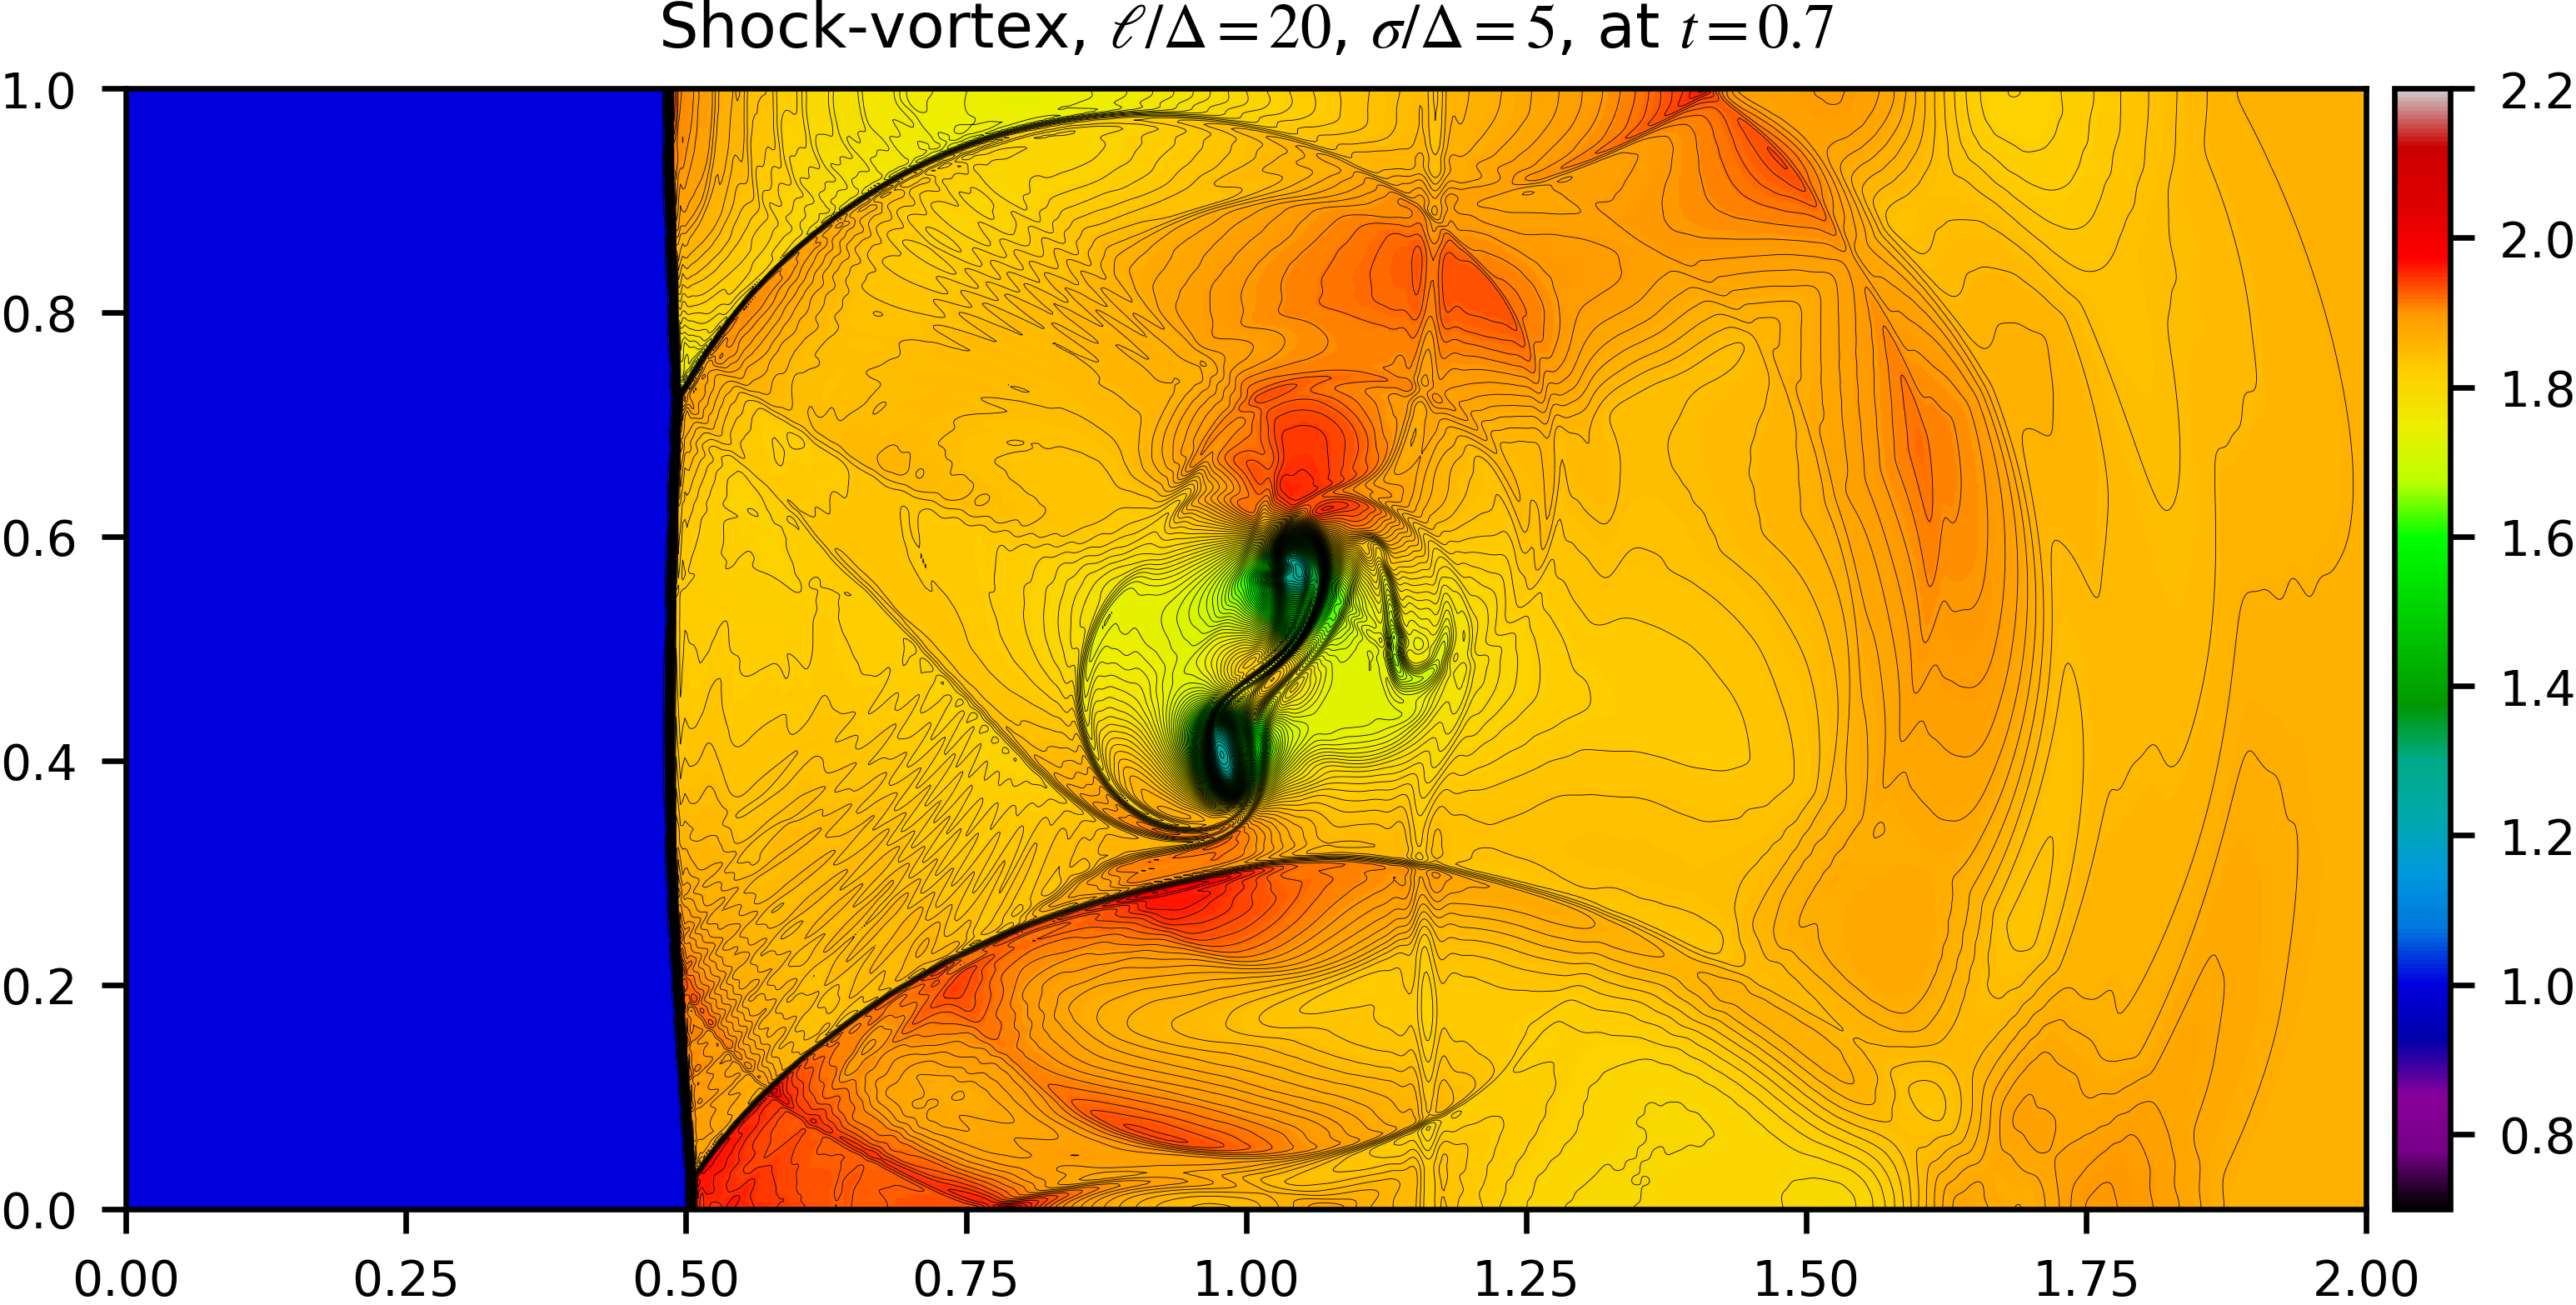
\includegraphics[width=0.95\textwidth]{fig/shockvortex_gp_ed20_sd5.png}
    \end{subfigure}
    \begin{subfigure}{120mm}
        \centering
        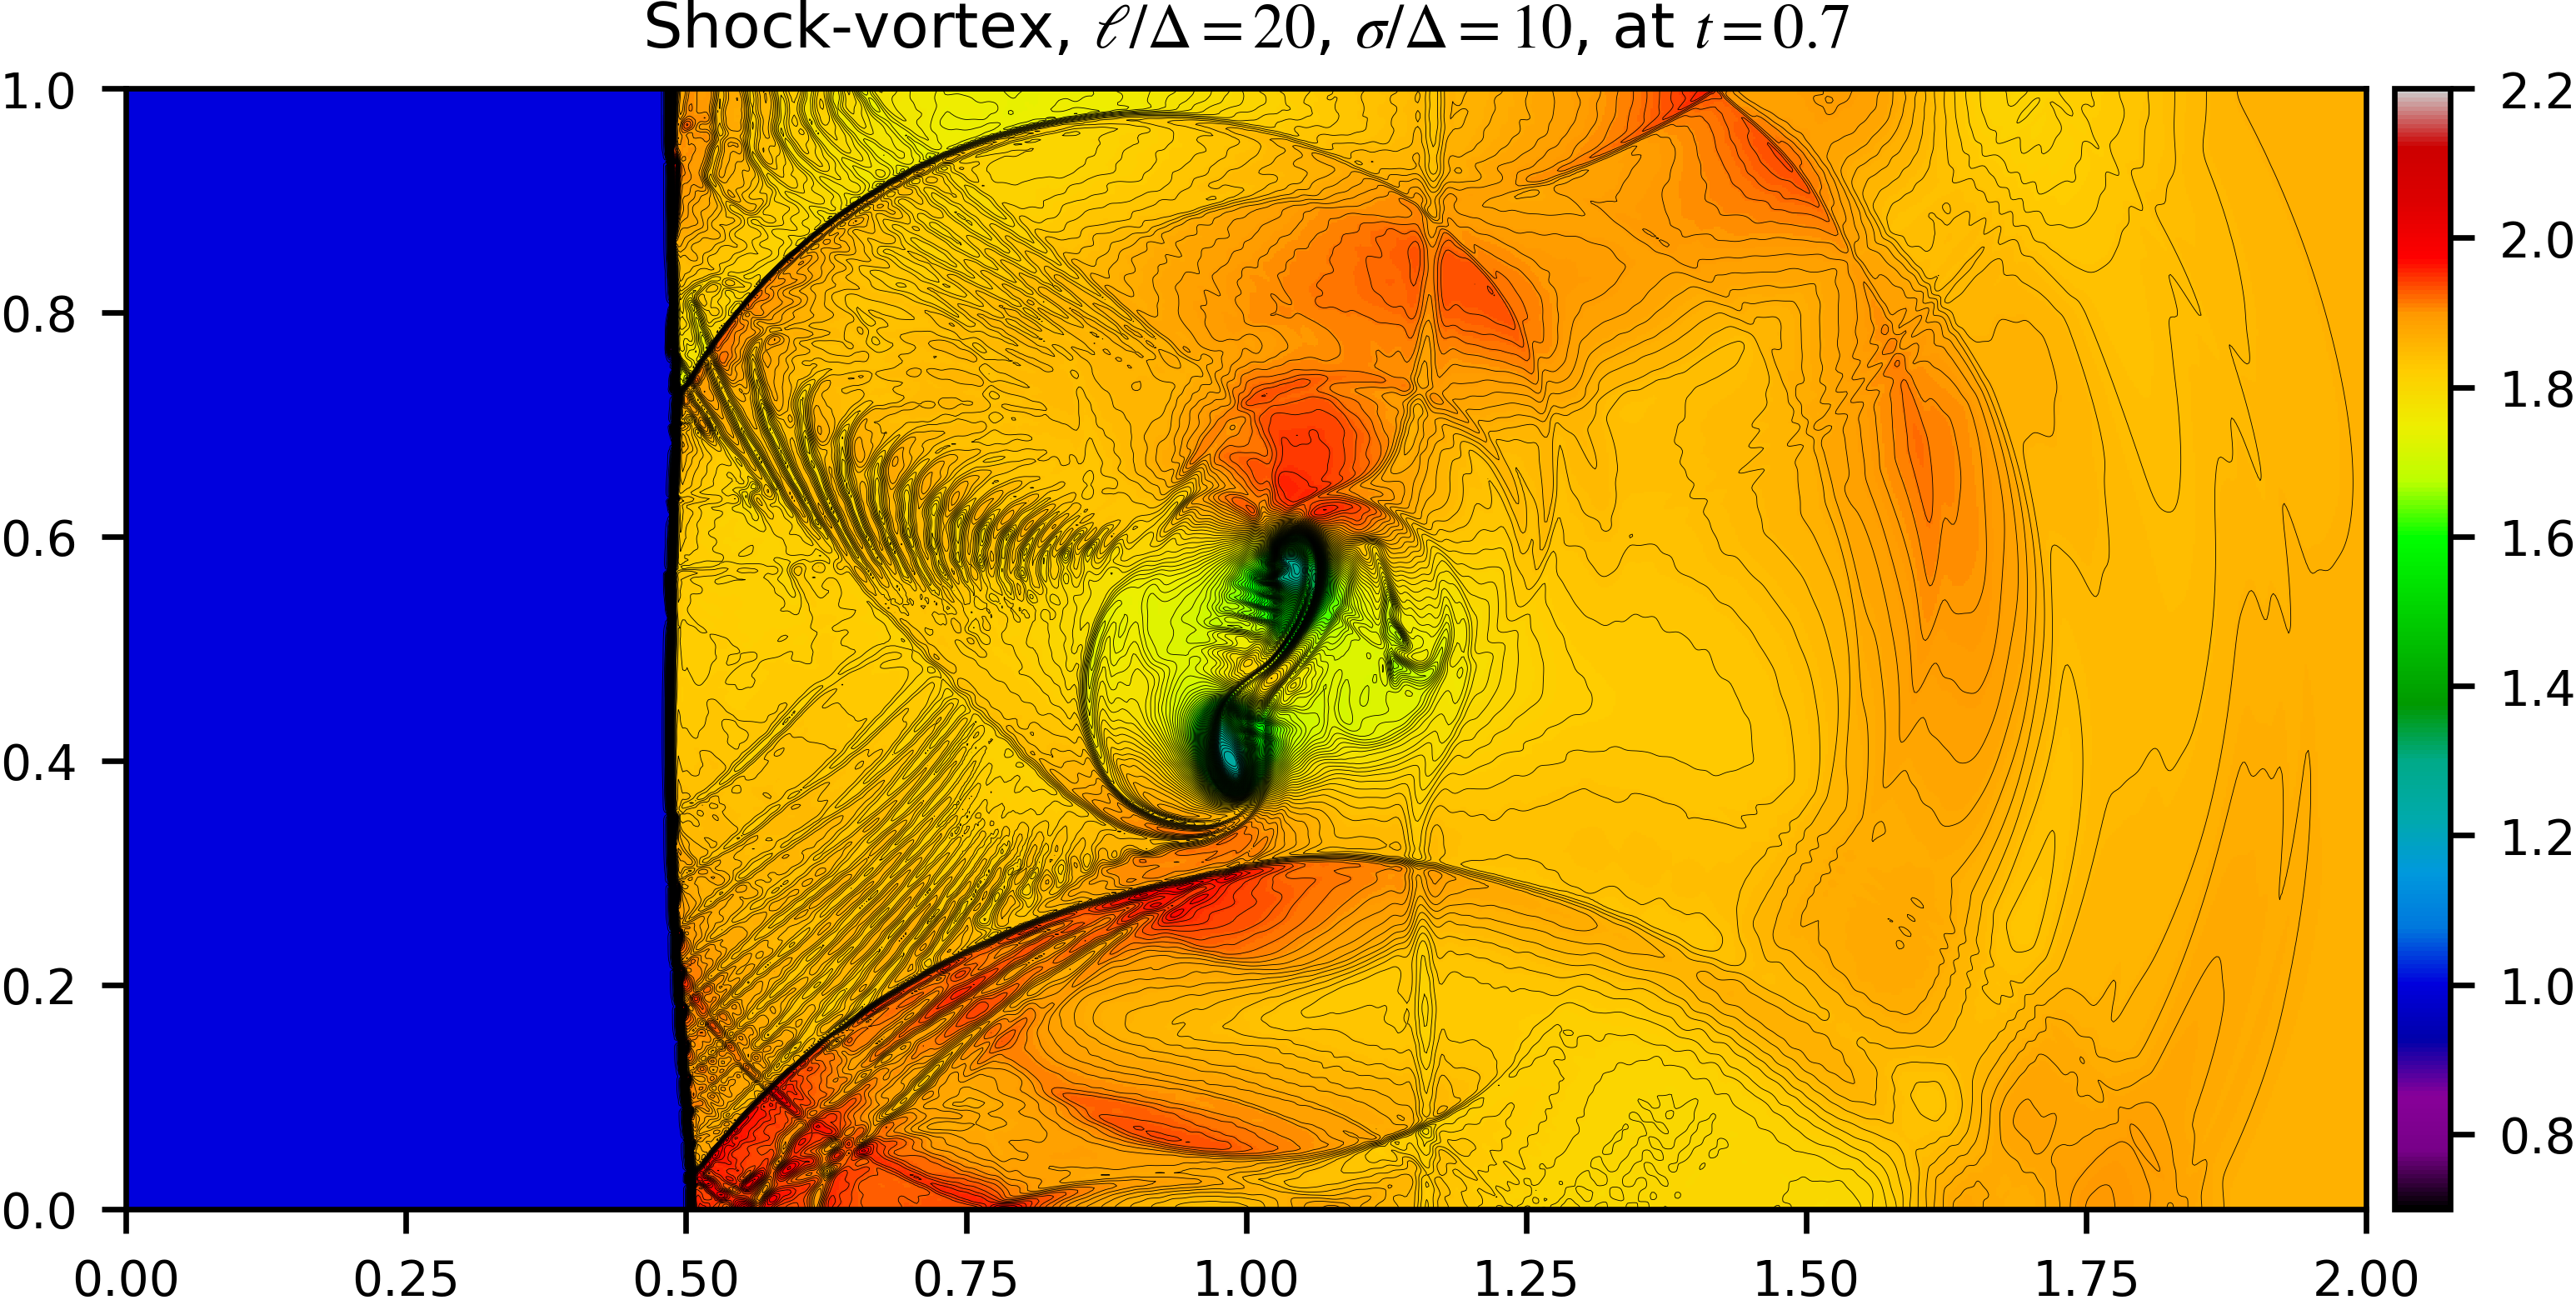
\includegraphics[width=0.95\textwidth]{fig/shockvortex_gp_ed20_sd10.png}
    \end{subfigure}
    \begin{subfigure}{120mm}
        \centering
        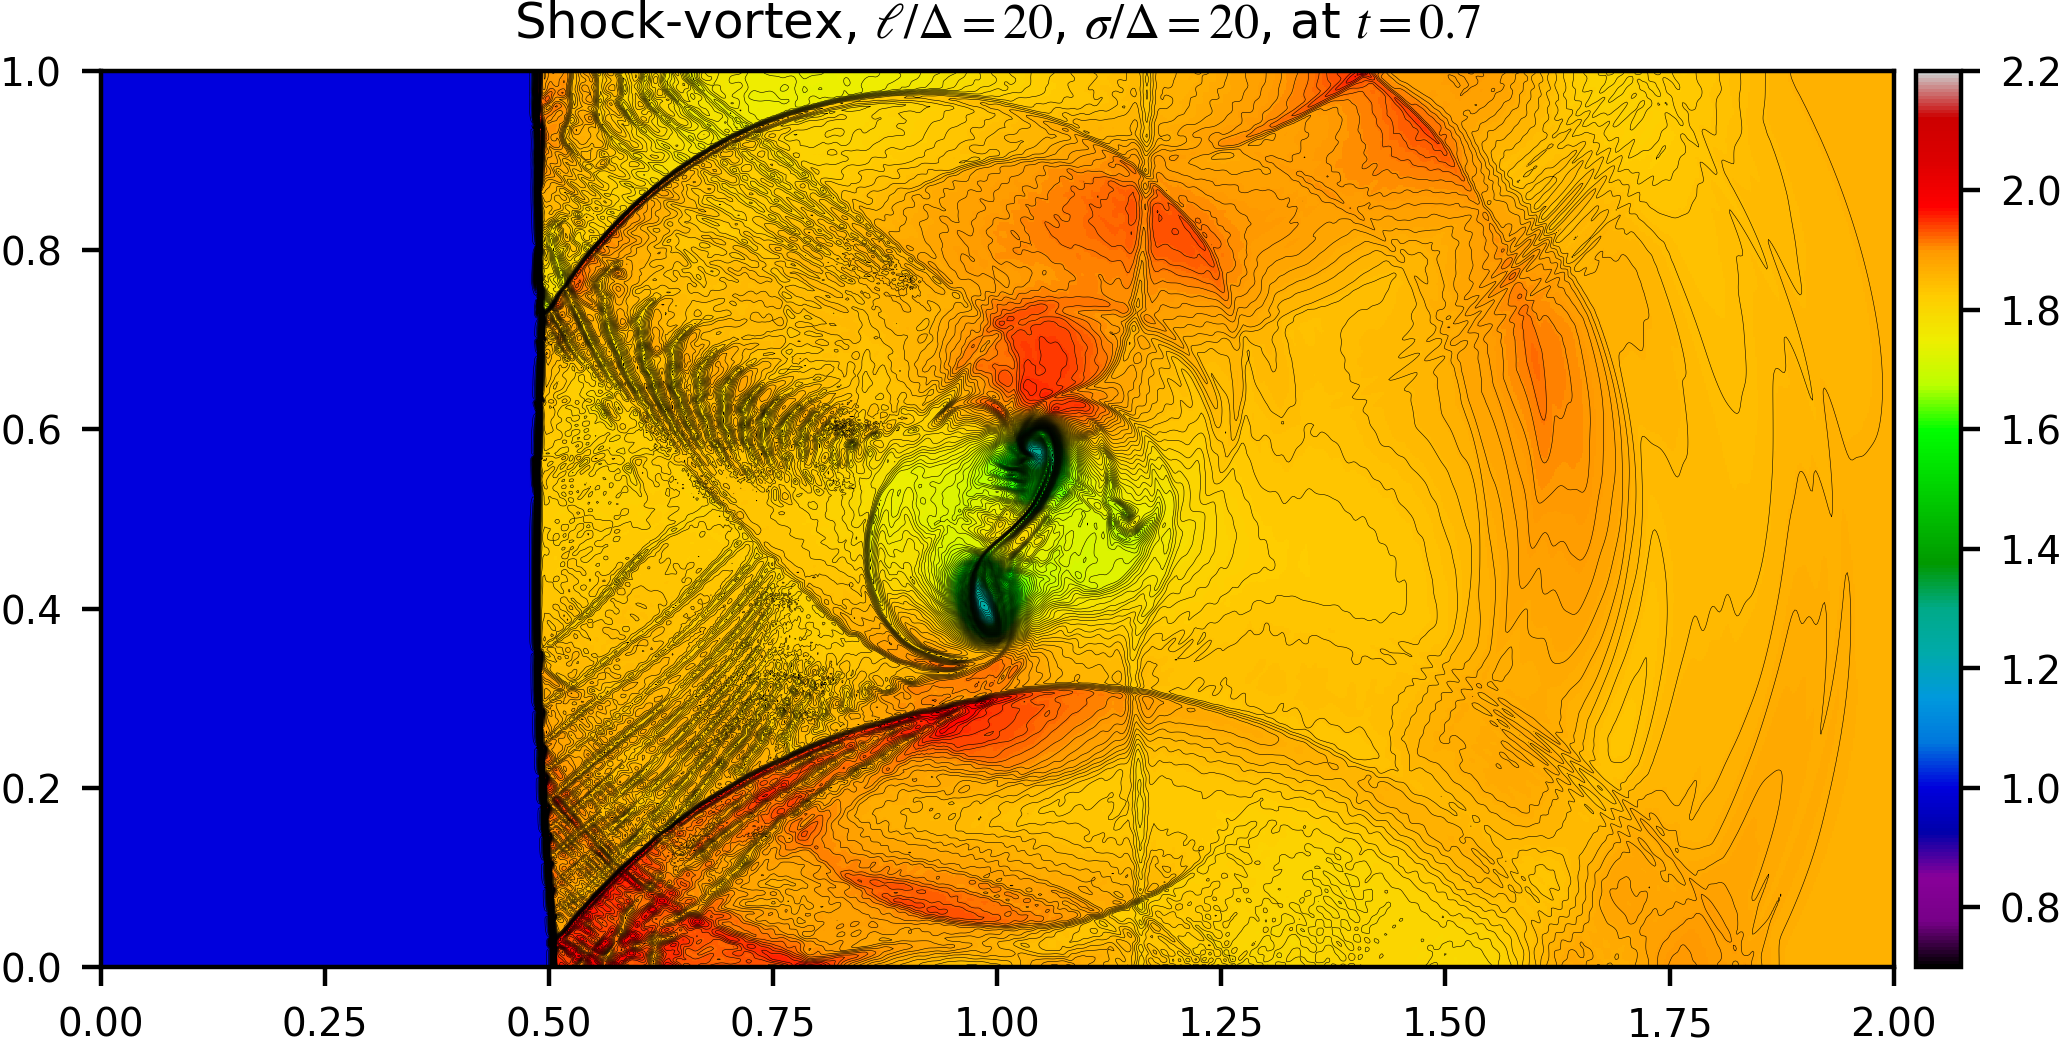
\includegraphics[width=0.95\textwidth]{fig/shockvortex_gp_ed20_sd20.png}
    \end{subfigure}
    \caption{The density colormaps of the strong shock vortex interaction problem.
        The GP-WENO (\( r = 2 \)) + SF-PIF3 method
        are used for all simulation runs
        on \( [1024 \times 512] \) grid resolution
        with varying hyperparameter, \( \sigma/\Delta \).
        The pseudo-colors represent the density map ranging between \( [0.75, 2.2] \),
        and 200 contour lines within the same range are over-plotted as solid black lines.
    }\label{fig:shockvortex}
\end{figure}

The results of the simulation of the GP-WENO method with varying \( \sigma \)
are presented in~\cref{fig:shockvortex}.
The SF-PIF3 method is used as a temporal method on a \( [1024 \times 512] \) grid resolution.
The obtained solutions with GP-WENO and SF-PIF3 methods are
well-comparable with the reference solution presented in~\cite{cheng2019two,galbraith5th}.
The GP hyperparameters are normalized with the grid scale \( \Delta \),
as suggested in~\cite{reyes2018new,reyes2019variable}.
The length-scale hyperparameters, \( \ell/\Delta = 20 \) is taken
based on the results of the previous section
(e.g., \( \ell/\Delta = 20 \) is equivalent to \( \ell = 1 \) with the vortex problem of \( 400 \times 400 \) resolution grid)
and various shock-capturing hyperparameters, \( \sigma/\Delta = 5, 10, \) and \( 20 \) are tested.

As shown in~\cref{fig:shockvortex}, the higher values of \( \sigma/\Delta \) is better
to capture the small-scale fluid structures, especially on the trailing waves of the vortex
around \( 0.5 \le x \le 1 \).
However, as discussed in~\cref{subsec:2drp_c3_weno} before,
identifying the numerical artifacts in the small-scale fluids is not feasible
without extensive numerical tests.
At a minimum, it is safe to say that the larger \( \sigma \) values
can produce less dissipative numerical solutions capturing the small-scale structures.


\chapter{Conclusion}
\label{ch:conclusion}

% \appendix % Uncomment if you have appendices. Add them below this exactly as you would a regular chapter.

\nocite{*}
\bibliographystyle{plain}
\singlespacing
\bibliography{dissertation}
\doublespacing

\end{document}
